\chapter{一种面向时空运动范围的轨迹相似性连接方法}

\section{引言}
随着智能手机等 GPS 设备的普及，对移动对象的查询问题受到了广泛关注，相关研究涵盖了连接（join）、范围查询、$k$NN 查询、相似性查询等多种类型。然而，由于采样频率不一致、位置采样可能存在误差，以及相邻采样点之间位置不可观测等因素，这类查询面临着诸多挑战。现有的相似性连接方法通常依赖于离散的位置采样点，难以刻画移动过程中的不确定性，从而可能遗漏具有实际意义的交互行为。

为了解决上述局限性，本文提出了一种新的方法——Intersection Similarity Join（IS-Join），该方法并非基于位置邻近性，而是根据对象运动范围的重叠程度来识别对象对。我们将运动范围定义为对象在给定时间段内可能经过的空间区域，并进一步提出了一种交集相似性度量来量化不同对象运动范围之间的重叠程度。

为了高效处理 IS-Join 查询，我们设计了一种带有重划分策略的 Hybrid Ball-tree 索引结构，以实现可扩展的候选对象过滤。此外，我们还引入了预检查（pre-checking）和剪枝（pruning）技术，以进一步降低计算开销。基于两个真实轨迹数据集的大量实验结果表明，IS-Join 在性能上显著优于精心设计的对比方法，运行时间最多可降低至原来的 $1/3$（即实现最高约 $3\times$ 的加速）。该研究为城市出行分析、交通监测、野生动物追踪以及接触追踪等应用场景开辟了新的可能性。
\subsection{研究背景与意义}
相似移动对象对的匹配问题，通常称为相似性连接（similarity join），是数据管理中的一项基础功能。该领域的现有研究工作~\cite{DBLP:journals/pvldb/Xu0B20,DBLP:journals/information/AlarabiBHA21,DBLP:journals/tkde/ShangCZJWK19,DBLP:journals/vldb/ShangCWJZK18,ding2025parallel} 通常将移动对象建模为一系列带时间戳的位置采样点，并基于这些采样点之间的空间邻近性来度量对象间的相似性。

然而，在真实场景中，出于隐私保护、商业因素、数据缺失以及部署成本高昂等原因，移动对象往往只能以较低的采样频率进行观测~\cite{DBLP:journals/air/KongCHWX23}，这使得相邻观测之间的位置信息不可获取。为了引入更高的灵活性，已有研究通过最小外接矩形（minimum bounding rectangle, MBR）来表示对象，并采用基于速度的表示模型来刻画其运动行为~\cite{DBLP:conf/icde/SistlaWCD97,DBLP:conf/sigmod/PatelCC04,DBLP:conf/sigmod/SaltenisJLL00,DBLP:conf/icde/ZhangLRB08,DBLP:journals/vldb/ZhangQLWW12}。另一类方法~\cite{DBLP:conf/mdm/BakalovHKT05} 则利用分段聚合近似（piecewise aggregate approximation, PAA）~\cite{DBLP:conf/vldb/YiF00} 将轨迹表示为符号序列，即将轨迹片段映射为来自预定义字母表的符号。

尽管上述方法在一定程度上提升了建模能力，现有表示方式仍然难以刻画采样点之间的运动过程，这一问题在稀疏采样轨迹场景下尤为突出。由此可能导致本应满足条件的结果对象对被错误地遗漏。因此，如何有效建模移动对象之间的运动交集关系，以及在海量移动对象数据下如何高效地发现所有交集，仍然是一个有待解决的开放性挑战。

在此背景下，我们提出了面向移动对象的交集相似性连接（Intersection Similarity Join，IS-Join）问题，通过引入运动范围来刻画对象在相邻观测样本之间可能访问的位置。具体而言，我们将对象的运动范围定义为其在某一时间点或给定时间区间内可能到达的空间区域。两个对象之间的交集相似性由其运动范围内特征的重叠程度来确定。

给定表 \texttt{MovingObject} 中的一组对象以及相似性阈值 $\theta$，我们以类似 SQL 的形式定义 IS-Join，如下所示~\footnote{为便于表示，我们以自连接（self-join）的形式定义 IS-Join。需要注意的是，本文提出的方法同样支持非自连接（non-self join）场景。}。

\begin{adjustwidth}{0.5in}{0in} \texttt{SELECT $o.id, o'.id$\\ FROM MovingObject AS $o$, MovingObject AS $o'$\\ WHERE $o.id<o'.id$ AND $IS(o,o',I) \geq \theta$} \end{adjustwidth}

每个对象 $o$ 由一个 $id$ 属性、两个位置坐标属性以及两个时间戳属性来表征，其中时间戳表示对象访问对应位置的时间。条件 $o.id<o'.id$ 用于避免重复比较。函数 $IS(o,o',I)$ 用于度量对象 $o$ 与 $o'$ 在时间区间 $I$ 内基于各自运动范围中特征重叠程度的交集相似性。参数 $\theta$ 为预先设定的相似性阈值。

IS-Join 问题面向多种应用场景，例如疾病防控、轨迹数据清洗、拼车推荐以及交通拥堵预测等~\cite{DBLP:journals/ral/VishnuARMB23,DBLP:conf/ijcai/LiCS20}。下面我们将讨论若干潜在的应用场景。



\textit{场景 1 —— 城市交通监测。} 特征集合可以包括道路路段、交叉路口以及交通信号灯等要素。交集相似性刻画了两辆车辆经历相似交通状况的可能性，有助于拥堵预测与交通优化。对于兴趣点（POI）和道路交叉口等点状特征，我们为每一个点分配一个唯一的 ID。为了将类似的方法应用于道路路段，我们将道路划分为等长度的子路段，并为每个子路段分配唯一的 ID。

\textit{场景 2 —— 野生动物迁徙。} 所定义的运动范围通过考虑栖息地、水源以及迁徙路线等特征，有助于识别共享的迁徙通道。此外，运动范围在节能的数据采集与准确的交互检测之间提供了一种折中方案~\cite{forrest2022moving}。

\textit{场景 3 —— 接触追踪。} 所定义的运动范围能够对潜在的接触事件进行估计，从而提升流行病监测系统的有效性。交集相似性可以帮助用户评估其感染风险，这在新冠疫情期间对于降低感染传播具有重要价值~\cite{DBLP:conf/ijcai/LiCSWLK022}。


  



\begin{figure}[htb]
    \centering
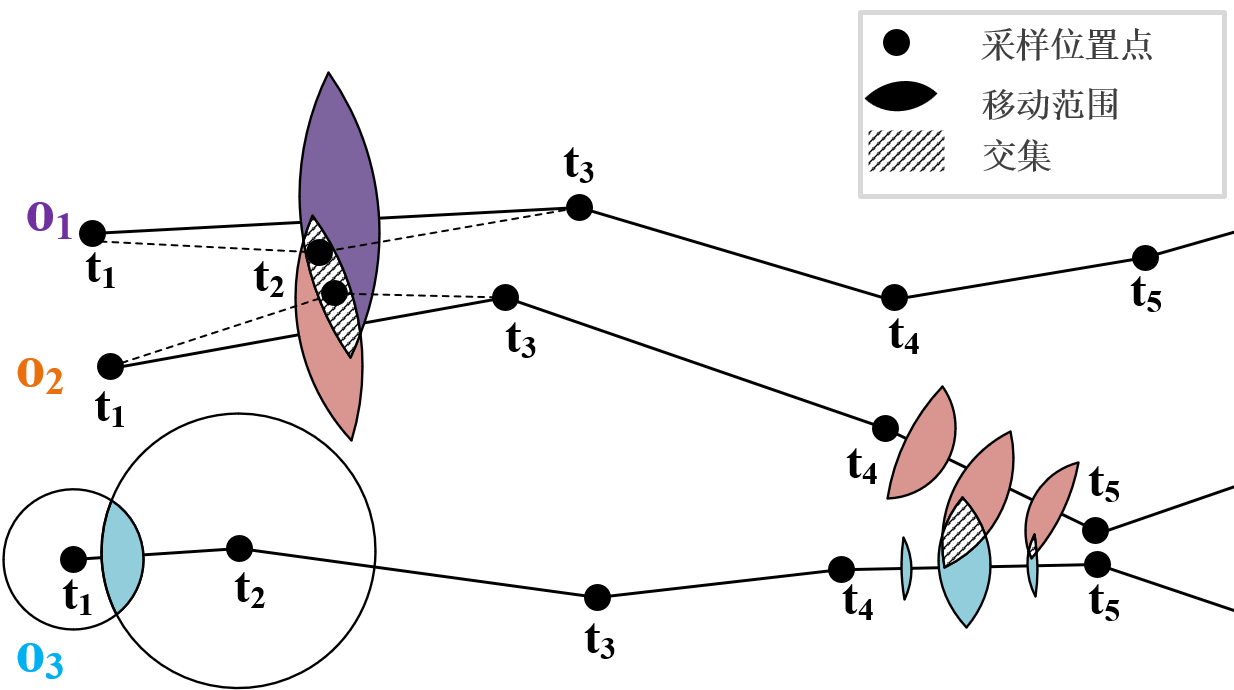
\includegraphics[width=1\columnwidth]{fig/section6/intro.png}
    \caption{IS-Join问题示例}
    \label{fig:intro}
\end{figure}

\textit{示例。} 如图~\ref{fig:intro} 所示，考虑三个移动对象 $o_1, o_2$ 和 $o_3$，它们在时间戳 $t_1$ 至 $t_5$ 之间均具有位置采样点。为简化说明，假设这些位置采样在时间上是对齐的。对象 $o_1$ 和 $o_2$ 在 $t_2$ 时刻的位置采样要么缺失，要么噪声过大而无法使用。如果仅通过判断位置采样之间的距离是否小于给定阈值来执行相似性连接，我们可能会错误地认为在时间区间 $[t_1, t_3]$ 内 $(o_1, o_2)$ 不是一个满足条件的结果对，尽管它们在 $t_2$ 时刻的实际距离可能低于该阈值。

通过考虑对象的运动范围，可以避免这种错误排除。以 $o_3$ 在 $t_1$ 和 $t_2$ 时刻的位置为例，$o_3$ 在时间点 $t\in[t_1,t_2]$ 内的运动范围为一个透镜形区域，其具体定义将在第~\ref{sec:statement} 节中给出。对象 $o_1$ 和 $o_2$ 在时间点 $t\in(t_1,t_3)$ 内的运动范围分别以紫色和棕色的透镜形区域表示。可以观察到，$o_1$ 与 $o_2$ 的运动范围在阴影区域内发生重叠，这表明它们可能存在潜在的位置交集。

接下来，我们关注时间区间 $[t_4, t_5]$。图中展示了 $o_2$ 和 $o_3$ 在区间 $[t_4,t_5]$ 内若干离散时间点上的一系列运动范围。区间 $[t_4,t_5]$ 的交集相似性被定义为该区间内各离散时间点交集相似性的平均值，具体定义将在后文的问题描述中进一步说明。给定一个时间区间和相似性阈值，IS-Join 问题旨在识别并返回在该时间区间内交集相似性大于或等于所给阈值的所有对象对。

据我们所知，这是首个在移动对象相似性连接研究中显式引入运动范围的工作。为了使 IS-Join 在实际中具有可行性，其算法必须在海量数据集上具备高效性和可扩展性。然而，IS-Join 问题的求解面临两个关键挑战。首先，在一个连续时间区间内计算精确的交集相似性在实际中是不可行的，因为这需要处理无限多个时间点。其次，现有的连接算法主要针对其他类型的查询而设计，无法直接支持 IS-Join。实验结果表明，即使在小规模数据集上，简单地改造这些方法也会导致严重的效率问题。为此，我们提出了一种由时间区间运动范围引导的解决方案。具体而言，我们设计了一种基于 HBall-tree 的连接算法，结合有效的重划分与剪枝技术，相较于精心设计的基线方法，平均运行时间可降低约 3 倍。


本文的主要贡献总结如下。

\begin{itemize}
\item 我们提出了一种新的问题——交集相似性连接（Intersection Similarity Join，IS-Join），并研究了可用于求解该问题的现有技术。不同于以往基于离散位置采样点邻近性来识别相似对象对的方法，本文首次识别运动范围感知相似性超过给定阈值的对象对。
\item 我们提出了一种由时间区间运动范围引导的高效 IS-Join 求解方案。为此，本文设计了一种混合 Ball-tree（Hybrid Ball-tree，HBall-tree）索引结构及其配套的剪枝增强技术。HBall-tree 能够高效地识别候选对象对，而剪枝增强技术则在处理早期阶段剔除不满足条件的对象对，从而显著提升查询性能。
\item 我们在两个真实世界数据集上进行了大量实验，对所提出的解决方案进行了深入分析，并验证了该方法在性能上显著优于精心设计的基线方法。
\end{itemize}

\subsection{相关工作}
\subsection{移动对象索引}
移动对象通常被表示为带时间戳的位置采样点~\cite{DBLP:conf/www/ZhengZXM09,DBLP:journals/vldb/LiNHLXZ23,DBLP:journals/debu/ZhengXM10}。R-tree~\cite{DBLP:conf/sigmod/Guttman84,DBLP:conf/sigmod/BrinkhoffKS93} 和 KD-tree~\cite{DBLP:journals/cacm/Bentley75,DBLP:journals/pvldb/ZhangCJOZ09} 是支持高效移动对象查询的两类经典索引结构。这类索引中的每个内部节点对应一个矩形区域，其子树包含位于该区域内的数据点。此外，M-tree~\cite{DBLP:conf/sebd/CiacciaPRZ97,DBLP:conf/vldb/CiacciaPZ97} 和 Ball-tree~\cite{DBLP:journals/jmlr/LiuMG06} 被设计用于高效处理圆形区域内的查询。Omohundro~\cite{omohundro1989five} 通过比较多种 Ball-tree 的构建方法，研究了构建时间与树结构质量之间的权衡关系。为提升索引结构的平衡性，Dolatshah 等人~\cite{DBLP:journals/corr/DolatshahHM15} 利用主成分分析来改进空间划分方式，从而确定更优的划分轴。另一项相关研究~\cite{DBLP:conf/dasfaa/ChaoHLZ021} 提出了面向移动对象的广义接触搜索查询。Zhang 等人~\cite{DBLP:conf/edbt/ZhangRSL21} 研究了接触相似性查询，并提出了用于索引的 ``UTM-tree''。然而，现有工作尚未基于运动范围来研究接触追踪问题，而这一点正是本文所关注的核心内容。

\subsection{轨迹相似性连接}
大量研究致力于轨迹相似性搜索与连接问题~\cite{DBLP:journals/vldb/LiangYWLCXL24,li2023relaxed,DBLP:journals/vldb/NutanongZTK10,DBLP:journals/vldb/WardH0Q14,chang2024trajectory,DBLP:conf/kdd/HanWYS021}。在这些研究中，Shang 等人~\cite{DBLP:journals/vldb/ShangCWJZK18} 采用线性组合的方式融合空间相似性与时间相似性。为降低系统负载，已有工作提出了基于速度的表示方法~\cite{DBLP:conf/icde/SistlaWCD97,DBLP:conf/sigmod/PatelCC04,DBLP:conf/sigmod/SaltenisJLL00}。Ding 等人~\cite{DBLP:journals/tkde/DingZWLBZL21} 提出了一种数据驱动的方法，利用真实历史轨迹数据挖掘实际可达区域来刻画问题。为了支持更灵活的轨迹相似性定义，Bakalov 等人~\cite{DBLP:conf/mdm/BakalovHKT05} 采用分段聚合近似（Piecewise Aggregate Approximation，PAA）~\cite{DBLP:conf/vldb/YiF00} 将轨迹表示为符号序列，并将 PAA 片段映射为来自预定义字母表的符号。他们构建了一种紧凑索引，用于高效评估近似连接，并通过后过滤步骤在加载最少轨迹数据的情况下对查询结果进行精化。Chen 等人~\cite{DBLP:conf/gis/ChenP09} 提出了一个通用的轨迹连接框架，涵盖距离连接和 $k$ 最近邻连接。此外，Tampakis 等人~\cite{DBLP:journals/tsas/TampakisDPT20} 提出了一种子轨迹连接查询，用于检索所有“最大化”的相似轨迹片段，从而识别“最大匹配”的子轨迹。尽管上述研究将相似性概念扩展到了单纯位置采样邻近性之外，但据我们所知，尚无工作研究基于运动范围的交集相似性连接问题，因此其现有解决方案并不适用于本文所提出的 IS-Join 问题。

\subsection{研究内容与挑战}
\subsection{研究成果与贡献}






\section{问题描述}


在本节中，我们首先定义移动对象的运动范围以及移动对象之间的交集相似性。随后，引入放宽交集相似性的概念，并对交集相似性连接问题进行形式化定义。本文中使用的主要符号汇总于表~\ref{tab:notation}。


\begin{table}[b]
    \centering
    \setlength{\tabcolsep}{8pt}% column separation
    \renewcommand{\arraystretch}{1}%row space 
    \begin{tabular}{ll}
        \hline
		\bfseries 符号 & \bfseries 含义 \\
        \hline
        $o$ & 一个移动对象  \\ 
        $s$ & 一个带时间戳的位置采样点  \\ 
        $[x,y],t$ & 坐标 / 时间戳  \\
        $I$ & 一个时间区间  \\ 
        $MR(\cdot)$ & 对象的运动范围 \\ 
        $dist(\cdot)$ & 距离度量函数 \\
        $\mathcal{F}(\cdot)$ & 运动范围的特征集合 \\ 
        $IS(\cdot)$ & 交集相似性度量\\
        $\theta$ & 交集相似性阈值 \\
        $\epsilon$ & 放宽划分参数 \\
        $T^\epsilon$  & 采样时间戳集合 \\
        $\mathcal{A}, \mathcal{B}$ & 两个移动对象集合  \\
        $\mathcal{R}$ & IS-Join 的结果集合 \\
        \hline
    \end{tabular}
    \caption{符号说明汇总}
    \label{tab:notation}
\end{table}




\begin{definition}[带时间戳的位置采样]
移动对象的一个带时间戳的位置采样表示为 $s=([x,y],t)$，其中 $[x,y]$ 表示空间坐标，$t$ 表示该位置被访问的时间戳。
\end{definition}


\begin{definition}[时间点运动范围]
\label{defi: point motion}
给定移动对象 $o$ 的两个位置采样点 $s_i = ([x_i, y_i], t_i)$ 和 $s_{j}=([x_j,y_j], t_j)$，以及最大速度 $v_{max}$，对象 $o$ 在时间 $t$（其中 $t \in [t_i, t_j]$）处的运动范围记为 $MR(o, t)$，其计算方式如公式~\ref{eq:timestamped motion range} 所示。函数 $dist(\cdot)$ 表示两个位置之间的距离度量。该运动范围呈透镜形状，如图~\ref{fig:lens} 所示，其两个半径 $r_i$ 和 $r_j$ 分别为 $v_{max}\cdot (t-t_i)$ 和 $v_{max}\cdot (t_j-t)$。
\begin{equation}    
\label{eq:timestamped motion range}
\begin{aligned}
MR(o,t) = \{ (x,y) \mid dist((x,y),(x_i,y_i)) \leq v_{max}\cdot(t-t_i)  \wedge \\ 
dist((x,y),(x_j,y_j)) \leq v_{max}\cdot(t_j-t)\}
\end{aligned}
\end{equation}
\end{definition}



\begin{figure}
    \centering
    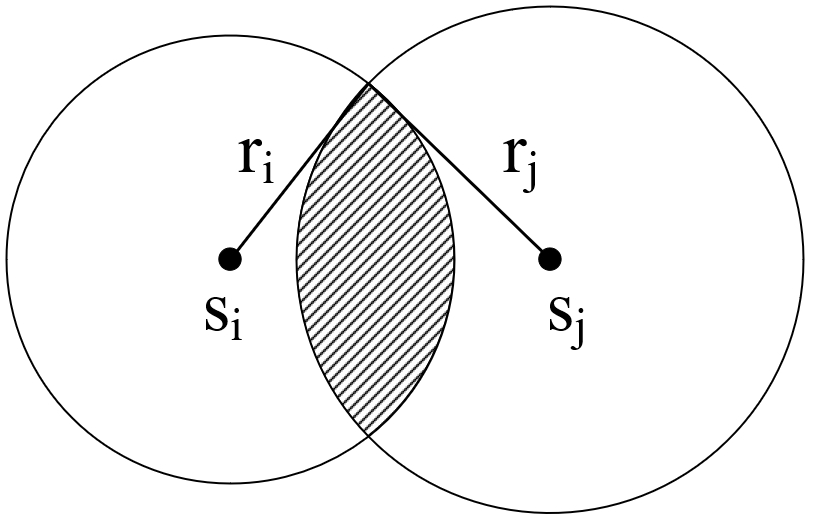
\includegraphics[width=0.5\columnwidth]{fig/section6/lens.png}
    \caption{Illustration of time-point motion range}
    \label{fig:lens}
\end{figure}


时间点运动范围的建模方式与已有研究保持一致~\cite{DBLP:conf/ssd/PfoserJ99,DBLP:conf/edbt/ZhangRSL21,trajcevski2010uncertain}。本文采用最大速度进行建模，以确保所估计的运动范围能够完全覆盖对象的真实运动轨迹。特别地，在采样时间戳处，对应的运动范围即退化为该时间戳的位置采样点本身。对于采样时间间隔异常较长（例如达到数小时）的对象，不在本文的分析范围之内。


\begin{definition}[运动范围特征]\label{defi: feature set}
设 $\mathcal{F}(o,t)$ 表示位于运动范围 $MR(o,t)$ 内的一组特定特征。示例包括运动范围的面积、范围内的兴趣点、经过的道路路段，以及地理空间区域或环境因素等。
\end{definition}



\begin{definition}[时间点交集相似性]\label{defi: point similarity}
对象 $o$ 与 $o'$ 在时间 $t$ 处的时间点交集相似性记为 $IS(o,o',t)$，其定义如公式~\ref{eq: time-point intersection similarity} 所示，用于度量二者特征集合之间的重叠程度。其中，$|\mathcal{F}(\cdot)|$ 表示位于 $MR(o,t)$ 内的特征集合大小，$\cap$ 表示特征集合之间的交集，该交集可根据具体应用场景表示共享的兴趣点、共同经过的道路路段，或重叠的运动范围区域等。相似性取值范围为 $[0,1]$，其中 1 表示特征集合完全重叠，0 表示不存在重叠。
%
\begin{equation}
    \label{eq: time-point intersection similarity}
    IS(o,o',t) = 
    \frac{|\mathcal{F}(o,t) \cap \mathcal{F}(o',t)|}{|\mathcal{F}(o,t)|}\times \frac{|\mathcal{F}(o,t) \cap \mathcal{F}(o',t)|}{|\mathcal{F}(o',t)|}
\end{equation}

\end{definition}

时间点交集相似性的定义基于如下考虑。首先，$MR(o,t)$ 描述了对象 $o$ 在时间 $t$ 处可能占据的位置范围，而 $\mathcal{F}(\cdot)$ 则表示该运动范围内的相关特征集合。采用乘积形式意味着两个因子都必须足够大，交集相似性才会取得较高值，从而保证只有在运动范围重叠程度高且特征相似性强这两个条件同时满足时，相似性得分才会较高。相比之下，经典的 Jaccard、取平均或取最小值等方法难以有效平衡运动范围重叠与特征相似性这两个方面。因此，$IS(o,o',t)$ 通过评估二者特征集合的重叠情况，刻画了对象 $o$ 与 $o'$ 之间发生交互的可能性。
 
\begin{definition}[时间区间交集相似性]\label{defi:interval similarity}
给定起始时间为 $t_s$、结束时间为 $t_e$ 的时间区间 $I$，我们将对象 $o$ 与 $o'$ 在区间 $I$ 上的交集相似性定义为该区间内时间点交集相似性的平均值，如公式~\ref{eq:interval intersection similarity} 所示。
\begin{equation}
    \label{eq:interval intersection similarity}
    IS(o,o',I) =\frac{\int_{t_s}^{t_e} IS(o,o',t) \, dt}{t_e-t_s}
\end{equation}
\end{definition}

计算时间区间交集相似性并非易事，因为由于时间区间的连续性，需要在无限多个时间点上评估时间点交集相似性。为在实际应用中对大规模移动对象数据提供一种可扩展的近似计算方式，并在不显著损失一般性的前提下，本文提出了一种放宽的定义。




\begin{definition}[$\epsilon$-放宽的时间区间交集相似性）]\label{defi:relaxed similarity}
给定一个较小的常数 $\epsilon$，我们对时间区间 $I=[t_s,t_e]$ 进行 $\epsilon$-采样，通过均匀采样得到一组时间点 $T^\epsilon=\{t_1^\epsilon,\ldots,t_m^\epsilon\}$，其中 $t_1^\epsilon=t_s$，$t_m^\epsilon=t_e$，且满足 $t_{i+1}^\epsilon-t_i^\epsilon=\epsilon$。随后，我们将 $\epsilon$-放宽的时间区间交集相似性定义为对象 $o$ 与 $o'$ 在所有采样时间点 $t^\epsilon\in T^\epsilon$ 上的时间点交集相似性的平均值，记为 $IS(o,o',I,\epsilon)$，其计算方式如公式~\ref{eq:relaxed similarity} 所示。
\begin{equation}
    \label{eq:relaxed similarity}
     IS(o,o',I,\epsilon) = \frac{\sum_{i=1}^{m} IS(o,o',t_i^\epsilon)}{m}
\end{equation}
\end{definition}


从本质上看，时间区间相似性的计算需要对多个时间点上的时间点交集相似性进行评估。在下文中，如无特殊说明，为表述简洁起见，我们使用“交集相似性”来指代 $\epsilon$-放宽的交集相似性。当 $\epsilon$ 趋近于 0 时，$IS(o,o',I,\epsilon)$ 将收敛到 $IS(o,o',I)$。

\textit{示例。}
图~\ref{fig:relaxed similarity example} 给出了一个时间区间交集相似性计算的示例。考虑时间区间 $I=(t_4,t_5)$，令 $\epsilon=|I|/4$，则采样得到的时间集合为 $T^\epsilon={t_4,t_4+\epsilon,t_4+2\epsilon,t_4+3\epsilon,t_5}$。两个移动对象 $o_2$ 和 $o_3$ 在 $T^\epsilon$ 中各采样时间点处均具有对应的时间点运动范围。在时间点 $t_4$ 和 $t_4+\epsilon$ 处，两者的运动范围不存在交集，因此 $IS(o_2,o_3,t_4)=0$ 且 $IS(o_2,o_3,t_4+\epsilon)=0$。在 $t_5$ 时刻，$o_2$ 与 $o_3$ 的位置采样点相同，从而得到 $IS(o_2,o_3,t_5)=1$。因此，区间 $I$ 上的 $\epsilon$-放宽时间区间交集相似性可计算为 $(0+0+IS(o_2,o_3,t_4+2\epsilon)+IS(o_2,o_3,t_4+3\epsilon)+1)/5$。其中，$IS(o_2,o_3,t_4+2\epsilon)$ 和 $IS(o_2,o_3,t_4+3\epsilon)$ 的取值依据公式~\ref{eq: time-point intersection similarity} 计算，该公式能够适应不同应用场景下的具体需求。


\begin{figure}
    \centering
    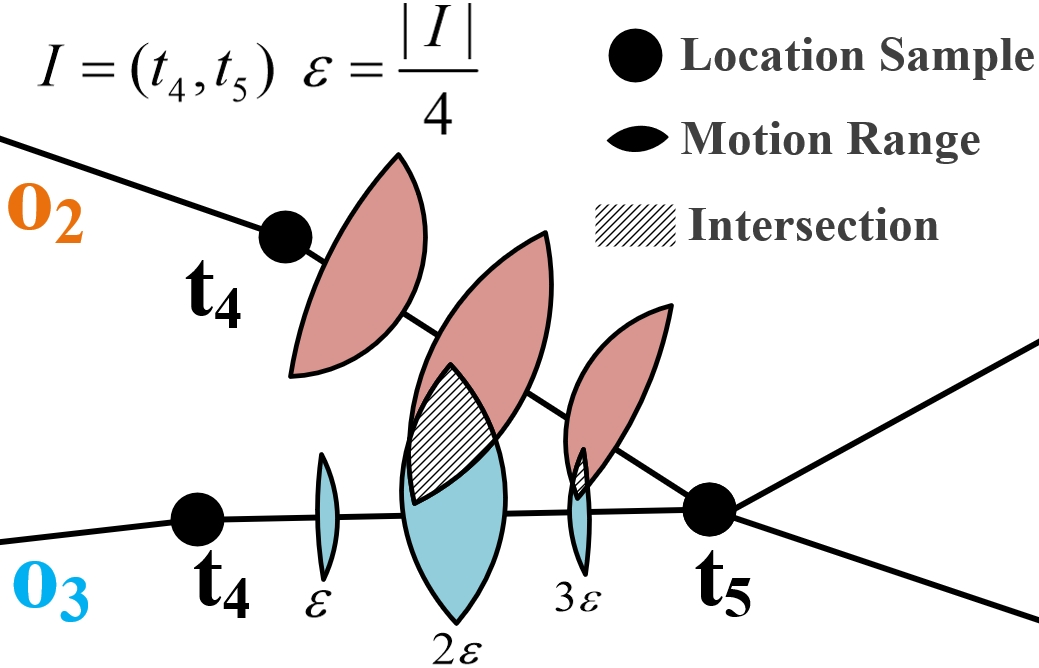
\includegraphics[width=0.6\columnwidth]{fig/section6/overall example.png}
    \caption{时间区间交集相似性的示意图}
    \label{fig:relaxed similarity example}
\end{figure}


我们在定义~\ref{defi:Tb-IS-Join} 中对交集相似性连接问题进行形式化描述。
\begin{definition}[IS-Join]\label{defi:Tb-IS-Join}
给定对象集合 $\mathcal{A}$ 和 $\mathcal{B}$、带有放宽划分参数 $\epsilon$ 的查询时间区间 $I$，以及相似性阈值 $\theta$，交集相似性连接（\underline{I}ntersection \underline{S}imilarity Join，IS-Join）旨在从这两个集合中找出所有交集相似性不小于 $\theta$ 的对象对所构成的集合 $\mathcal{P}$，即对于任意 $(o_i,o_j)\in (\mathcal{A}\times \mathcal{B})\setminus \mathcal{P}$，均有
$(IS(o_i,o_j,I,\epsilon)<\theta)$。
\end{definition}






\section{运动范围引导的匹配方法}

为高效地回答 IS-Join 查询，我们提出了一种由时间区间运动范围引导的匹配方法。在时间区间阶段，我们首先进行预检查，以判断两个对象的时间点运动范围之间是否存在交集。具体而言，我们定义时间区间运动范围 $MR(o,I)$，用于刻画对象 $o$ 在区间 $I$ 内可能到达的所有位置。如果 $MR(o, I)\cap MR(o', I)=\emptyset$，则可推出 $IS(o,o',I,\epsilon)=0$，从而对对象对 $(o,o')$ 进行剪枝。为高效判定 $MR(o,I)\cap MR(o',I)=\emptyset$，我们提出了一种新的混合 Ball-tree（Hybrid Ball-tree，HBall-tree）结构。同时，我们引入了一种基于交集相似度上界的剪枝增强方法，以进一步剔除不满足条件的对象对，从而细化整体处理流程。在精化阶段，计算运动范围内特征的交集以度量交集相似度。我们首先介绍基于时间区间运动范围的预检查策略，随后给出基于混合 Ball-tree 的连接算法（HBJ-Join）。

\subsection{时间区间预检查}\label{sec:inter pre-check}

本节介绍时间区间运动范围的概念，并给出具有理论保证的预检查策略。

\begin{definition}[时间区间运动范围]\label{defi:interval motion}
给定移动对象 $o$ 的两个带时间戳的位置样本 $s_i = ([x_i, y_i], t_i)$ 和 $s_{j}=([x_j,y_j], t_j)$，以及在 $t_i$ 与 $t_j$ 之间的最大速度 $v_{max}$，对象 $o$ 在时间区间 $I=[t_i,t_j]$ 内的运动范围，记为 $MR(o,I)$，被定义为对象 $o$ 在区间 $I$ 内可能到达的空间区域。
\end{definition}

定理~\ref{theorem:motion} 给出了计算 $MR(o,I)$ 的方法。

\begin{theorem}\label{theorem:motion}
对象 $o$ 的运动范围 $MR(o,I)$ 是由公式~\ref{eq:ellipse} 表示的一个椭圆区域。椭圆的中心点记为 $(x_c, y_c)$，由公式~\ref{eq:center} 计算得到；椭圆的旋转角度记为 $\alpha$，由公式~\ref{eq:angle} 计算，其中 $a$ 和 $b$ 分别表示半长轴和半短轴。
\begin{equation}
    \label{eq:ellipse}
    \begin{aligned}
 \left[\frac{(x-x_c)\cos\alpha+(y-y_c)\sin\alpha}{a}\right]^2+\\
    \left[\frac{(x_c-x)\sin\alpha+(y-y_c)\cos\alpha}{b}\right]^2 = 1
    \end{aligned}
\end{equation}
\begin{equation}
    \label{eq:center}
    \begin{aligned}
    x_c = \frac{x_i+x_{j}}{2}, \quad y_c=\frac{y_i+y_{j}}{2},\\
    a = \frac{v_{max}\cdot (t_{j}-t_i)}{2}, \\
    b=\frac{\sqrt{v_{max}^2\cdot (t_{j}-t_i)^2-(x_{j}-x_i)^2-(y_{j}-y_i)^2}}{2}
    \end{aligned}
\end{equation}
\begin{equation}
\label{eq:angle}
    \alpha = \arctan\!\left(\frac{y_{j}-y_i}{x_{j}-x_i}\right)
\end{equation}
\end{theorem}

\begin{proof} 
对象 $o$ 在时间区间 $I$ 内能够行进的最大距离为 $(t_j-t_i)\cdot v_{max}$，该结论同时适用于欧氏空间和路网空间。给定两个位置样本 $s_i$ 和 $s_j$，对象 $o$ 在某一具体时间点 $t$ 的运动范围可由公式~\ref{eq:timestamped motion range} 定义。需要注意的是，椭圆上任意一点到其两个焦点的距离之和为常数 $2a$。当 $v_{max}\cdot (t_j-t_i)=2a$ 时，从 $t_i$ 到 $t_j$ 的所有可能到达位置构成一个以 $(x_i, y_i)$ 和 $(x_j, y_j)$ 为焦点的椭圆区域，如图~\ref{fig:ellipse} 所示。我们对时间区间运动范围的建模方式与已有研究保持一致~\cite{DBLP:conf/edbt/ZhangRSL21,trajcevski2010uncertain}。
\end{proof}

\begin{figure}[tbp]
    \centering
    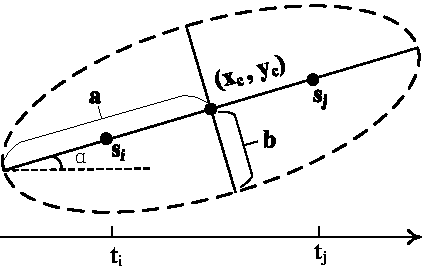
\includegraphics[width=0.6\columnwidth]{fig/section6/ellipse.pdf}
    \caption{时间区间运动范围示例}
    \label{fig:ellipse}
\end{figure}

基于定理~\ref{theorem:pre-checking}，我们提出了一种预检查策略：若 $MR(o,I)\cap MR(o',I)=\emptyset$，则可以在早期阶段安全地剪枝对象对 $(o,o')$，从而避免对特征集合（例如 POI、运动范围面积等）进行不必要的交集计算。

\begin{theorem}\label{theorem:pre-checking}
给定两个对象 $o$ 和 $o'$，若 $MR(o,I)\cap MR(o',I)=\emptyset$，则 $IS(o,o',I,\epsilon)=0$。
\end{theorem}

\begin{proof}
对于对象 $o$ 和 $o'$，如果它们在时间区间 $I$ 内的时间区间运动范围不相交，则在 $I$ 内任意时间点上，$o$ 与 $o'$ 的时间点运动范围都不可能发生重叠。由于与各自时间点运动范围相关的特征集合 $P(o,t)$ 和 $P(o',t)$ 在整个区间 $I$ 内均不存在交集，因此在区间 $I$ 上的交集相似度为 0。
\end{proof}

为了判断两个时间区间运动范围是否相交，一种直接的方法是计算它们的两两距离。具体而言，若距离
$dist(MR(o,I),MR(o',I))$ 大于 $MR(o,I).a + MR(o',I).a$，则两个运动范围不相交。其中，
$dist(MR(o,I),MR(o',I))$ 表示 $MR(o,I)$ 与 $MR(o',I)$ 中心点之间的距离，$a$ 表示运动范围的半长轴。
这种直接方法在进行一对一比较时需要 $O(\mathcal{A}\times \mathcal{B})$ 的时间复杂度，计算代价较高。

\label{sec:ball-tree}
\begin{figure*}[htbp]
    \centering
    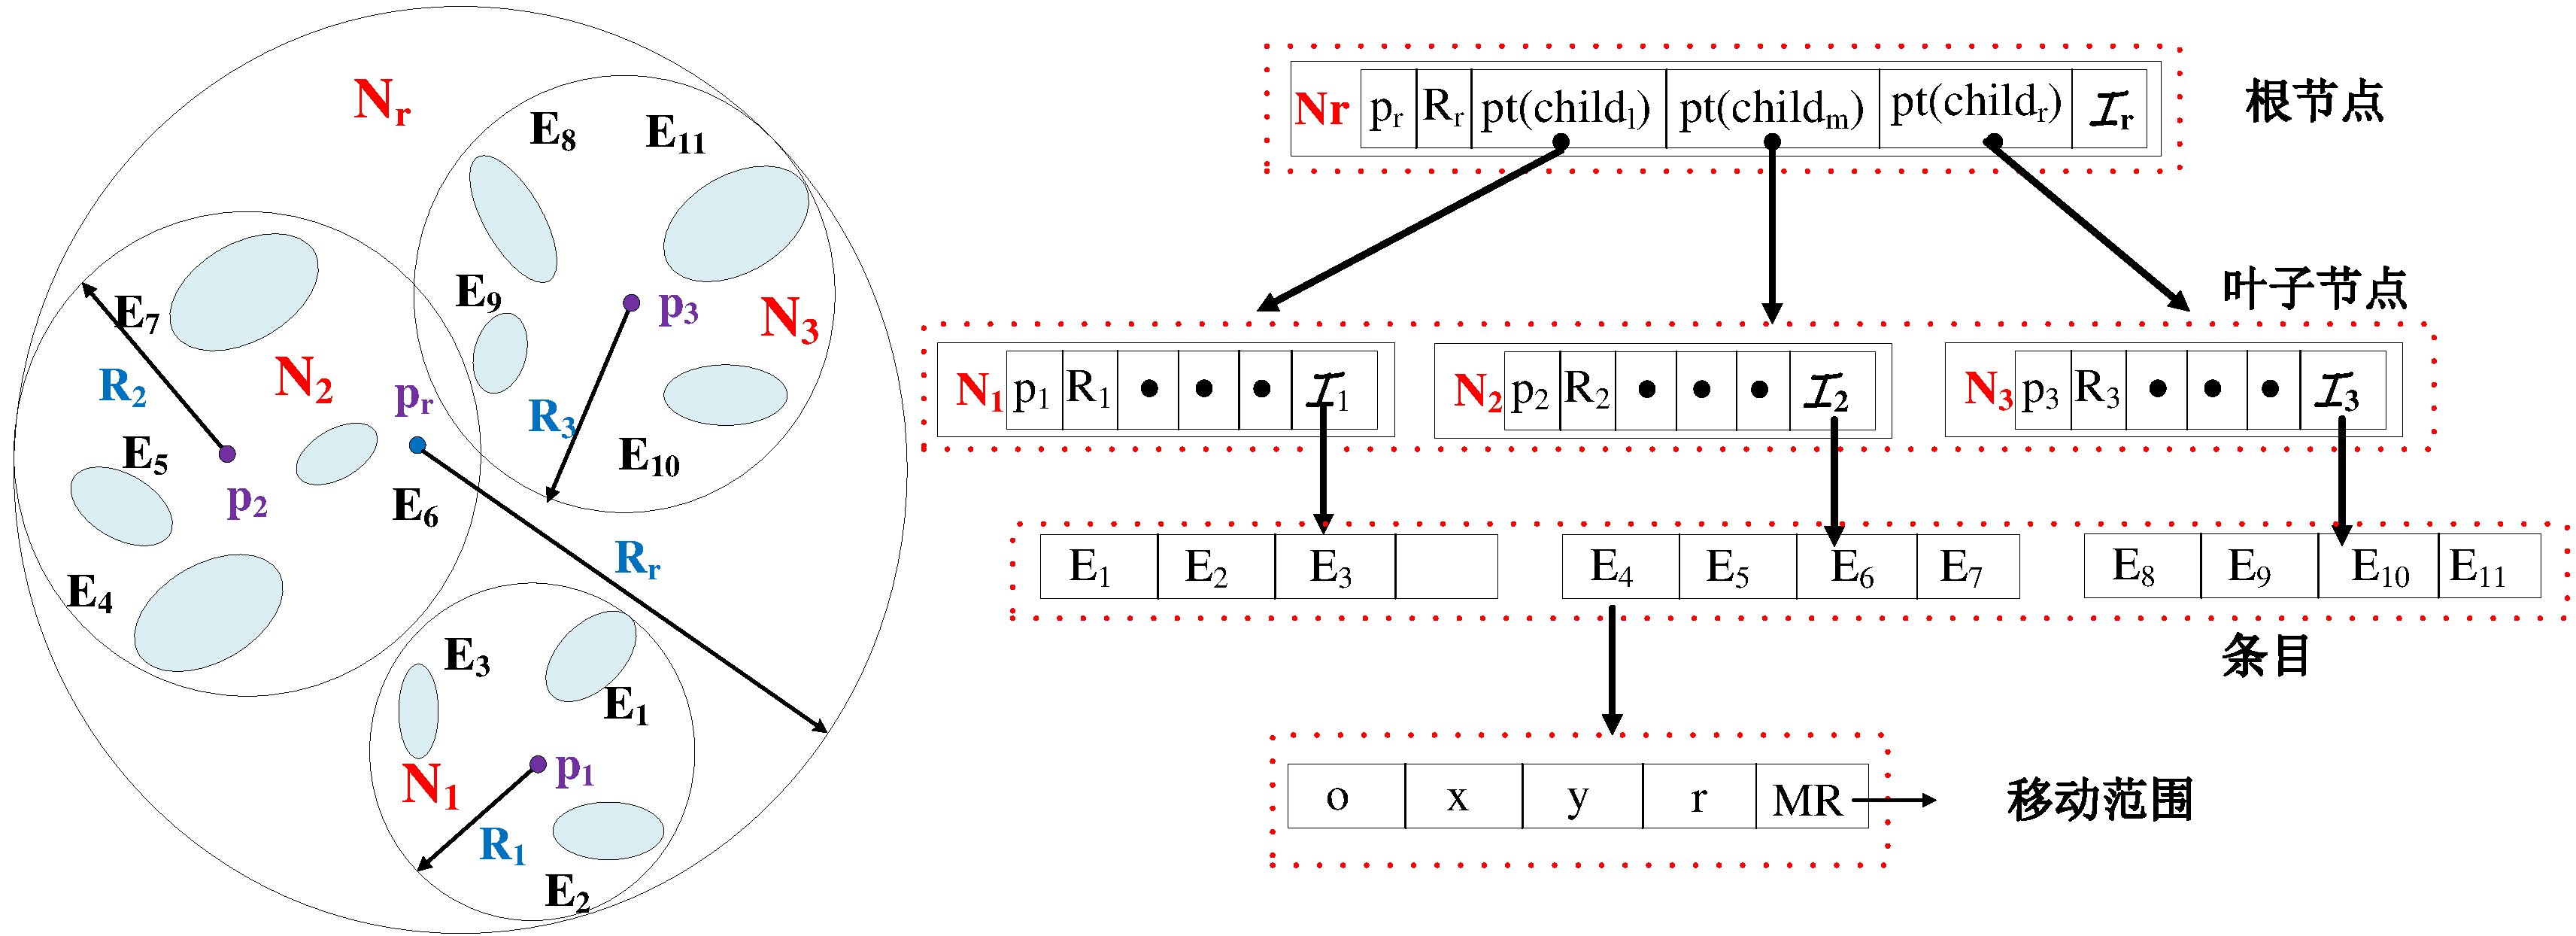
\includegraphics[width=1\textwidth]{fig/section6/ball-tree.pdf}
    \caption{混合 Ball-tree 的示意图}
    \label{fig:ball-tree}
\end{figure*}

```latex
\subsection{基于 HBall-tree 的交集预检查}
我们提出了一种混合 Ball-tree（Hybrid Ball-tree，HBall-tree），这是一种面向高效预检查的改进型索引结构，并展示了其如何提升“过滤–精化”过程的整体效率。

\subsubsection{HBall-tree}
\label{sec:hballtree}
我们选择 Ball-tree~\cite{omohundro1989five,DBLP:journals/jmlr/LiuMG06,DBLP:conf/uai/Moore00} 作为基础索引结构，这是因为相较于 R-tree~\cite{DBLP:conf/sigmod/Guttman84} 和四叉树~\cite{DBLP:journals/csur/Samet84} 等索引，Ball-tree 在处理类圆对象时表现更优~\cite{DBLP:conf/edbt/ZhangRSL21,DBLP:conf/sebd/CiacciaPRZ97,DBLP:conf/vldb/CiacciaPZ97}。然而，当将 Ball-tree 应用于 IS-Join 查询时，仍然存在两个关键局限性。首先，Ball-tree 主要面向点或圆级别的最近邻搜索设计，无法直接支持时间区间运动范围的索引。其次，其划分过程未考虑数据点的分布情况，可能导致划分不均衡，从而形成高度不平衡的树结构~\cite{DBLP:journals/corr/DolatshahHM15}。

为了解决第一个问题，我们将每个时间区间运动范围近似为一个圆~\cite{DBLP:conf/edbt/ZhangRSL21}。具体而言，该圆以时间区间运动范围的中心为圆心，其半径等于半长轴长度。该近似方式简化了时间区间运动范围的表示，使我们能够直接利用现有针对圆形对象设计的空间索引结构。其关键推论在于：如果两个近似圆不相交，则其对应的时间区间运动范围也必然不相交。该推论构成了我们过滤策略的基础，从而能够高效识别不可能发生交集的对象对。

为了解决第二个问题，我们提出了混合 Ball-tree（HBall-tree），这是一种能够考虑数据分布特性的全新索引结构。图~\ref{fig:ball-tree} 给出了 HBall-tree 的示意图。每个时间区间运动范围被表示为
$E=\{o,x,y,r,MR(o,I)\}$，
其中 $(x,y)$ 和 $r$ 分别表示近似圆的中心和半径，$o$ 表示对象标识符。与原始 Ball-tree 每个非叶节点仅包含两个子节点不同，HBall-tree 通过一种重新划分（repartition）技术，使得每个父节点最多可以拥有三个子节点。每个节点的结构表示为
$N=\{p,R,pt(child_l),pt(child_m),pt(child_r),\mathcal{I}\}$，
其中 $p$ 表示节点 $N$ 所覆盖的时间区间运动范围的中心点，$R$ 表示能够包围节点 $N$ 中所有条目（即圆）的半径，$pt(\cdot)$ 为指向子节点的指针，$\mathcal{I}$ 表示该节点中包含的时间区间运动范围集合。HBall-tree 中的插入策略、分裂策略以及枢轴点选择均遵循已有研究中的成熟方法~\cite{DBLP:conf/uai/Moore00}。当某一子划分中的对象数量低于预定义阈值（即生成新子节点所需的最小对象数）时，子划分过程终止。

\subsubsection{HBall-tree 的重新划分策略}
直观上，更加平衡的树结构通常能够在搜索过程中减少节点访问次数。重新划分方法的整体思想如下：对于每一个初始划分，我们评估其两个子划分中的点数差异是否超过重新划分阈值 $\beta$（$\beta \in (0,1)$）。如果差异超过该阈值，则保留点数较少的子划分，并将点数较多的子划分进一步划分为两个新的子划分。考虑一个节点 $N$，初始时 $N.child_m=\emptyset$。当较大的子划分规模至少以比例 $\beta$ 超过较小子划分时，即触发重新划分。例如，当 $|N.child_l.\mathcal{I}|>|N.child_r.\mathcal{I}|$，且
$\frac{|N.child_l.\mathcal{I}|-|N.child_r.\mathcal{I}|}{|N.child_r.\mathcal{I}|} \ge \beta$，
则触发重新划分。从理论上看，较小的重新划分阈值会使初始子树更容易被重新划分，从而增加三叉节点的数量，使树结构更加平衡。然而，三叉节点数量的增加也可能导致节点访问次数上升，因此需要在树高与三叉节点数量之间进行权衡。

对于非叶节点，初始划分基于 $N.\mathcal{I}$ 中选取的两个最远点进行。具体而言，树构建过程中两个最远点的选取步骤如下：(i) 随机种子点：从 $N.\mathcal{I}$ 中随机选择一个点作为初始种子；(ii) 第一个最远点：在数据集中找到距离该种子点最远的点；(iii) 第二个最远点：在数据集中找到距离第一个最远点最远的点。设这两个最远点分别为 $N.child_l.p$ 和 $N.child_r.p$，我们计算二者的中点，并在 $N.\mathcal{I}$ 中选取距离该中点最近的中心点，记为 $p_m$。点数较少的子划分被视为稳定划分，而我们对点数较多的子划分进行重新划分。具体地，若 $|N.child_l.\mathcal{I}|>|N.child_r.\mathcal{I}|$，则使用 $p_m$ 和 $N.child_l.p$ 将 $N.child_l.\mathcal{I}$ 中的运动范围重新划分为两个新的子划分，其中一个保留在 $N.child_l.\mathcal{I}$，另一个分配给 $N.child_m.\mathcal{I}$；反之，若 $|N.child_l.\mathcal{I}|<|N.child_r.\mathcal{I}|$，则使用 $p_m$ 和 $N.child_r.p$ 对 $N.child_r.\mathcal{I}$ 进行重新划分，一个子划分保留在 $N.child_r.\mathcal{I}$，另一个分配给 $N.child_m.\mathcal{I}$。最终，重新划分将原有的两个子划分扩展为三个子划分，新生成的子划分由 $N.pt(child_m)$ 索引。该重新划分技术带来了两方面优势：（1）降低树高与划分数量：通过提升平衡性，减少树的高度并最小化划分数量；（2）提升搜索效率：更加平衡的树结构能够减少树节点访问次数，从而提高搜索效率。
```
\subsection{基于 HBall-tree 的 Join}
我们提出了一种基于 HBall-tree 的 Join 算法。为了进一步提升效率，我们引入了一种剪枝增强方法，利用交集相似度的上界来进一步剔除不满足条件的对象对，从而优化整体处理流程。

\subsubsection{剪枝增强策略}
由于运动范围交集形状的不规则性，直接计算两个特征集合 $\mathcal{F}(o,t)$ 与 $\mathcal{F}(o',t)$ 的交集并非易事。给定时间点 $t$，若 $MR(o,t)\cap MR(o',t)\neq \emptyset$，当其中一个对象的运动范围完全被另一个对象覆盖时，$IS(o,o',t)$ 取得其最大值。基于这一观察，公式~\ref{eq:t-IS-ub} 给出了 $IS(o,o',t)$ 的一个上界。将公式~\ref{eq:t-IS-ub} 代入公式~\ref{eq:relaxed similarity}，可得到公式~\ref{eq:I-IS-ub1}，用于估计 $IS(o,o',I,\epsilon)$ 的上界。若 $IS(o,o',I,\epsilon)_{ub}<\theta$，则可以安全地剪枝对象对 $(o,o')$。

    \begin{equation}
    \label{eq:t-IS-ub}
    IS(o,o',t)_{ub} = 
   \frac{\min(|\mathcal{F}(o,t)|,|\mathcal{F}(o',t)|)}{\max(|\mathcal{F}(o,t)|,|\mathcal{F}(o',t)|)}\ge IS(o,o',t)
\end{equation}

    \begin{equation}
    \label{eq:I-IS-ub1}
     IS(o,o',I,\epsilon)_{ub} = \frac{\sum_{i=1}^{m} IS(o,o',t_i^\epsilon)_{ub}}{m}
\end{equation}

\begin{algorithm}[!h]
    \caption{$HBJ(\mathcal{A},\mathcal{B},N_r,I,\epsilon,\beta,\theta)$}
    \label{alg:ball filter}
    
    \Input{
    两组移动对象，$\mathcal{A}$ 和 $\mathcal{B}$；\newline
    HBall-tree 的根节点 $N_r$；\newline
    时间间隔 $I$；\newline
    松弛参数 $\epsilon$；\newline
    重分区阈值 $\beta$；\newline
    交集相似度阈值 $\theta$。
    }
    \Output{
    IS-Join 结果，$\mathcal{R}$。
    }
    
    \textbf{初始化:} $\mathcal{R} \leftarrow \emptyset$；
    
    \For(\tcc*[f]{遍历所有移动对象}){$o \in \mathcal{A}$}{
        $\mathcal{L} \leftarrow \{N_r\}$；
    
        \While(\tcc*[f]{BFS 遍历 HBall-tree}){$\mathcal{L} \neq \emptyset$}{
            $N \leftarrow \mathcal{L}.pop()$；
    
            \If(\tcc*[f]{非叶子节点分支}){$N$ 是非叶子节点}{
                \For(\tcc*[f]{遍历子节点}){$N_c \in N.pt(child)$}{
                    \If{$dist(o, N_c) \leq N_c.R + o.r$}{
                        $\mathcal{L}.push(N_c)$；
                    }
                }
            }
            \Else(\tcc*[f]{叶子节点处理}){
                \For(\tcc*[f]{遍历叶子节点对象}){$E \in N.\mathcal{I}$}{
                    \If{$dist(o, E) > E.r + o.r$}{
                        $prune(o, E.o)$;\tcp*[f]{预检查策略}
                    }
                    \If{$IS(o, E.o, I, \epsilon)_{ub} < \theta$}{
                        $prune(o, E.o)$;\tcp*[f]{剪枝增强策略}
                    }
                    \If{$IS(o, E.o, I, \epsilon) \geq \theta$}{
                        $\mathcal{R} \leftarrow \{\mathcal{R}, (o, E.o)\}$;\tcp*[f]{精炼步骤}
                    }
                }
            }
        }
    }
    \textbf{return} $\mathcal{R}$；
    \end{algorithm}



\subsubsection{算法细节}
算法~\ref{alg:ball filter} 给出了基于 HBall-tree 的 Join 算法（HBJ-Alg）的伪代码。该算法的输入包括两个移动对象集合、HBall-tree 的根节点、重分区阈值以及交集相似度阈值；输出结果为交集对象对集合 $\mathcal{R}$。初始时，$\mathcal{R}$ 为空（第 1 行）。对于每一个 $o\in\mathcal{A}$，我们使用列表 $\mathcal{L}$ 存储可能与 $MR(o,I)$ 发生交集的候选节点，初始时 $\mathcal{L}$ 仅包含根节点 $N_r$（第 3 行）。HBall-tree 通过插入对象集合 $\mathcal{B}$ 的时间区间运动范围构建完成。

当 $\mathcal{L}$ 非空时，算法调用 $\mathcal{L}.pop()$ 取出一个节点 $N$（第 5 行）。随后，在“圆级别”执行基于 HBall-tree 的过滤，以识别潜在的交集候选（第 6--9 行）。具体而言，我们检索 HBall-tree 中满足 $dist(o,N_c)\leq R+r_q$ 的节点，从而判断 $MR(o,I)$ 与 $N_c$ 之间是否可能存在交集。若 $N$ 为非叶节点，则检查其子节点。对于每个子节点 $N_c$，若对象 $o$ 与 $N_c$ 的距离不大于二者半径之和，则将 $N_c$ 压入优先队列（第 8--9 行）。

若 $N$ 为叶节点，则遍历 $N.\mathcal{I}$ 中的所有条目。对于每个条目 $E$，计算 $(E.x,E.y)$ 与 $(MR(o,I).x_c,MR(o,I).y_c)$ 之间的欧氏距离 $dist(o,E)$。若 $dist(o,E)>E.r+o.r$，则可安全剪枝 $(o,E.o)$（第 12--13 行）。否则，继续执行进一步的剪枝操作，即剪枝增强策略（第 14--15 行）。仅对保留下来的对象对，才进行精确的交集相似度计算，即利用公式~\ref{eq: time-point intersection similarity} 计算多个时间点的交集相似度（第 16--17 行）。最终返回结果集合 $\mathcal{R}$（第 18 行）。

\subsubsection{时间复杂度}
HBall-tree 的构建时间复杂度为 $O(|\mathcal{B}|\times \log|\mathcal{B}|)$。预检查阶段的时间复杂度为 $O(|\mathcal{A}|\times\log|\mathcal{B}|)$。设 $\mathcal{C}'$ 为候选集合，则候选精化阶段的时间复杂度为 $O(|\mathcal{C}'|\times |I|/\epsilon\times p)$。因此，HBJ-Alg 的总体时间复杂度为
\[
O\big((|\mathcal{A}|+|\mathcal{B}|)\times\log|\mathcal{B}| + |\mathcal{C}'|\times |I|/\epsilon\times p\big).
\]
HBJ-Alg 得益于增强的剪枝策略，显著减少了需要进行精化计算的候选对象对数量。











\section{实验研究}

\subsection{实验设置}
\subsubsection{数据准备}
实验研究~\footnote{代码已开源：\url{https://github.com/likemelike/IS-Join}} 在两个真实世界的轨迹数据集上进行。第一个数据集 Geolife \cite{DBLP:conf/huc/ZhengLCXM08,DBLP:journals/debu/ZhengXM10} 包含来自 182 名用户、历时四年的 17,621 条轨迹，涵盖了多种户外移动行为，包括日常通勤以及购物、骑行等休闲活动。第二个数据集 Porto~\cite{DBLP:journals/tits/Moreira-MatiasGFMD13} 包含在葡萄牙波尔图市 19 个月内记录的超过 170 万条出租车轨迹。Porto 数据集的轨迹以 15 秒为采样间隔记录，而 Geolife 的采样频率则不固定。时间戳被限定在 24 小时范围内，而不考虑具体日期，因为大多数城市交通出行行为具有日常重复性。我们将对象的最大速度 $v_{max}$ 定义为其在给定时间区间内观测到的最高速度。确定 $v_{max}$ 的真实取值或最优设置超出了本文的研究范围。为保证实际应用相关性，我们剔除了采样时间间隔过大（超过一小时）的极端轨迹，因为这类轨迹在现实应用中实用性有限，因此不纳入本研究。我们注意到，在隧道等环境中 GPS 信号可能较弱甚至完全丢失，从而导致异常位置或较低的采样率。尽管对这类异常值进行显式建模超出了本文的研究范围，但我们的数据预处理流程通过基于经度、纬度、轨迹长度和速度等约束过滤异常轨迹，从而在一定程度上缓解了这些影响。预处理后，Geolife 数据集中保留了 18,670 条轨迹中的 12,015 条有效轨迹，Porto 数据集中保留了 1,710,670 条轨迹中的 1,392,385 条。随后，从数据集中随机选取两个包含相同数量移动对象的对象组。

\subsubsection{对比算法}
我们将所提出的方法与一种设计良好的基于 M-tree 的连接算法~\cite{DBLP:conf/edbt/ZhangRSL21}（见附录）进行对比，记为 MBJ-Alg，作为基线方法。为评估剪枝增强策略的影响，我们还测试了不包含剪枝增强策略的 HBJ-Alg，记为 HBJ-Alg\#。在效率评估方面，我们同时衡量剪枝率和 CPU 时间。剪枝率定义为 $1- |C|/|O|^2$，其中 $C$ 表示候选集。CPU 时间表示算法每一轮的平均运行时间。此外，我们还评估了不采用重新划分策略的 HBJ-Alg，记为 HBJ-Alg$*$。

\begin{table}[tb]
	\centering
    \begin{tabular}{l|rr}
	\toprule
    \hline
		&\textbf{Geolife}&\textbf{Porto}\\
	\hline
        $|O|$ & \{4,6,8,10,12\} $\times 10^3$ & \{1,2,3,4,5\} $\times 10^4$  \\ 
        & 8K (默认) & 10K (默认) \\
    \hline
        $|I|$ & \{10s, 20s, 30s, 40s, 50s\}  & \{15s,  30s, 45s, 60s, 75s\} \\
		   & 30s (默认) & 45s (默认) \\
      \hline
        $|\mathcal{F}|$ & \{2, 4, 6, 8, 10\}$\times 10^5$  & \{1, 2, 3, 4, 5\}$\times 10^5$  \\
		   & 600K (默认) & 100K (默认) \\
     \hline
        $\epsilon$ & \{$\frac{|I|}{2}$,   $\frac{|I|}{4}$, $\frac{|I|}{6}$, $\frac{|I|}{8}$, $\frac{|I|}{10}$\}   & \{$\frac{|I|}{2}$,   $\frac{|I|}{4}$, $\frac{|I|}{6}$, $\frac{|I|}{8}$, $\frac{|I|}{10}$\}  \\
		   & $\frac{|I|}{6}$ (默认) & $\frac{|I|}{6}$ (默认) \\
\bottomrule
    \end{tabular}
    \caption{评估参数设置}
    \label{tb:algorithm_para}
\end{table}

\subsubsection{参数设置}
参数设置如表~\ref{tb:algorithm_para} 所示。M$^\ast$-tree 和 HBall-tree 的叶节点容量均设置为 10。默认情况下，重新划分阈值 $\alpha$ 设为 0.5。在实验中，特征集合 $\mathcal{F}$ 由随机生成的兴趣点（POIs）构成。具体而言，我们首先确定所有轨迹的最小和最大经度与纬度值，在该空间范围内使用均匀分布随机生成固定数量的 POIs。默认情况下，在 Porto 数据集的坐标范围内生成 100,000 个 POIs，在 Geolife 数据集中生成 600,000 个 POIs。默认距离度量采用欧氏距离。所有方法均使用 Java 实现，并在配备 AMD Ryzen 5 CPU（3.6GHz）和 32GB 内存的 Ubuntu 系统上进行评测，采用单线程执行。除非另有说明，实验结果均为 20 次独立实验的平均值，每次实验使用不同的轨迹数据和特征集。


\subsection{Performance Evaluation}

\subsubsection{剪枝有效性评估}
首先，我们在默认参数设置下考察各算法的剪枝有效性。实验结果如表~\ref{tb:prune} 所示。通过比较 MBJ-Alg 与 HBJ-Alg 的候选集规模和剪枝率可以发现，在 Geolife 和 Porto 数据集上，HBJ-Alg 的候选集规模分别仅为 MBJ-Alg 的 0.5\% 和 2.3\%。这些结果表明，所提出的方法能够显著压缩搜索空间。

\begin{table}[tb]
    \begin{tabular}{|p{6cm}|p{3cm}|p{3cm}|}
        \hline
        \diagbox{指标/数据集}{方法} & MBJ-Alg & HBJ-Alg  \\
        \hline
        候选集规模（Geolife） & 6540764 & 28862\\
        \hline
        剪枝率（Geolife） & 89.7800\% & 99.9549\%\\
        \hline
        候选集规模（Porto） & 2142988 & 50072\\
        \hline
        剪枝率（Porto） & 97.8570\% & 99.9499\%\\
        \hline
    \end{tabular}
    \caption{剪枝性能}
    \label{tb:prune}
\end{table}

接下来，我们在不同参数设置下进一步评估所提出算法的性能。需要说明的是，在改变某一个参数时，其余参数均保持为默认值。

\subsubsection{移动对象基数的影响}
我们研究了不同移动对象基数 $|O|$ 对算法性能的影响。直观上，较大的 $|O|$ 会导致需要处理更多的时间区间运动范围，因此所有算法的运行时间都将随之增加。首先，我们评估了 MBJ-Alg、HBJ-Alg 以及 HBJ-Alg$*$ 的索引构建时间，结果如图~\ref{img:vary_num_ctime} 所示。可以清楚地看到，MBJ-Alg 的构建开销明显高于 HBJ-Alg。与 HBJ-Alg$*$ 相比，HBJ-Alg 表现出相近且略有提升的性能。这一改进主要得益于 HBJ-Alg 中的再划分技术：尽管在触发再划分时会引入额外计算开销，但该技术能够减少总体分区数量，从而在整体上有助于降低构建时间。

接下来，我们分析了所提出算法在 IS-Join 查询中的总运行时间。随着移动对象数量的增加，由于交集候选对数量增多，计算负载显著上升，所有算法的时间复杂度均随之提高。从图~\ref{img:vary_num_ftime} 可以观察到，随着数据规模的扩大，MBJ-Alg 的 CPU 时间显著增加。例如，在 Geolife 数据集包含 12K 个移动对象、Porto 数据集包含 50K 个移动对象时，MBJ-Alg 的查询时间分别超过 3 秒和 30 秒，计算开销较大。相比之下，HBJ-Alg 和 HBJ-Alg\# 始终优于 MBJ-Alg，尤其在大规模数据集上表现出更高的效率。值得注意的是，HBJ-Alg 的 CPU 时间几乎没有明显退化，充分体现了所提出方法的良好可扩展性。此外，与 HBJ-Alg\# 相比，HBJ-Alg 的运行时间降低了约 30\%，突出了剪枝增强策略所带来的性能提升。具体而言，在 Geolife 数据集包含 12,000 个移动对象、Porto 数据集包含 50,000 个移动对象时，HBJ-Alg 相比 MBJ-Alg 在 Geolife 上实现了 $3.1x$ 的加速，在 Porto 上实现了 $3.3x$ 的加速。

\begin{figure}[tb]
    \centering
    \subfloat[]{
    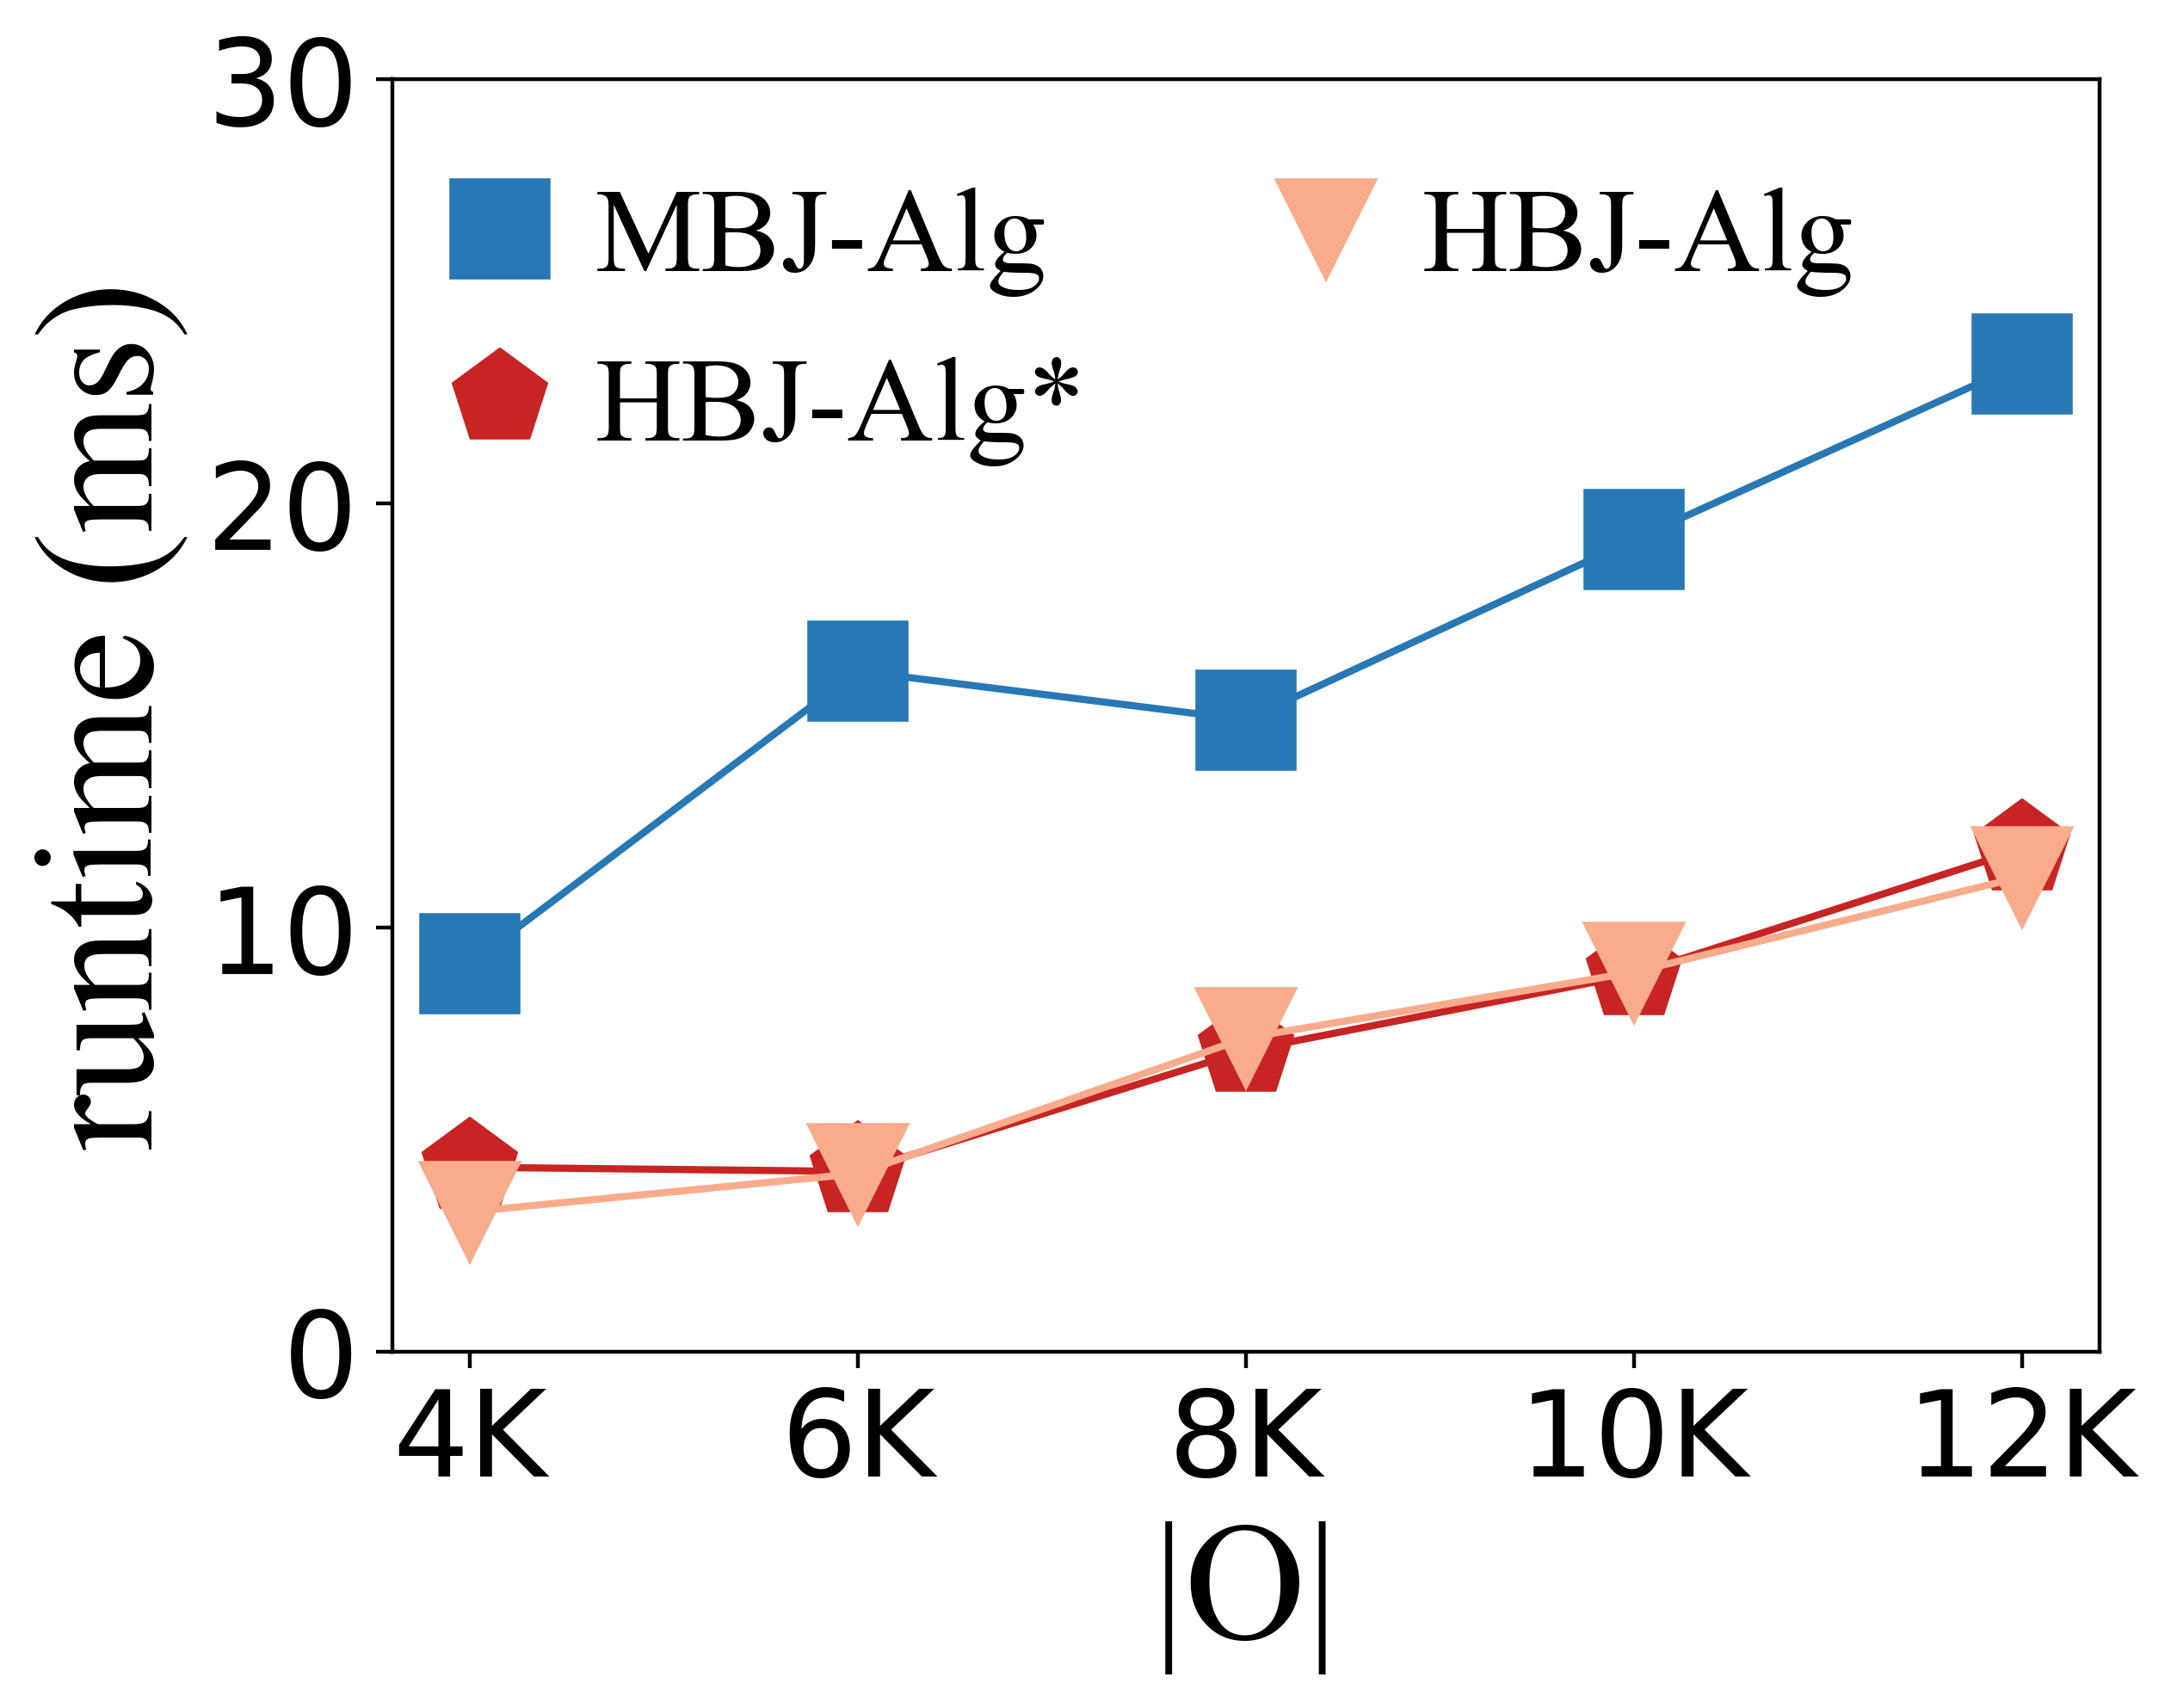
\includegraphics[width=0.5\textwidth]{fig/section6/geo-num-ctime.png}
    \label{geo-num-ctime}
}% 
\subfloat[]{
    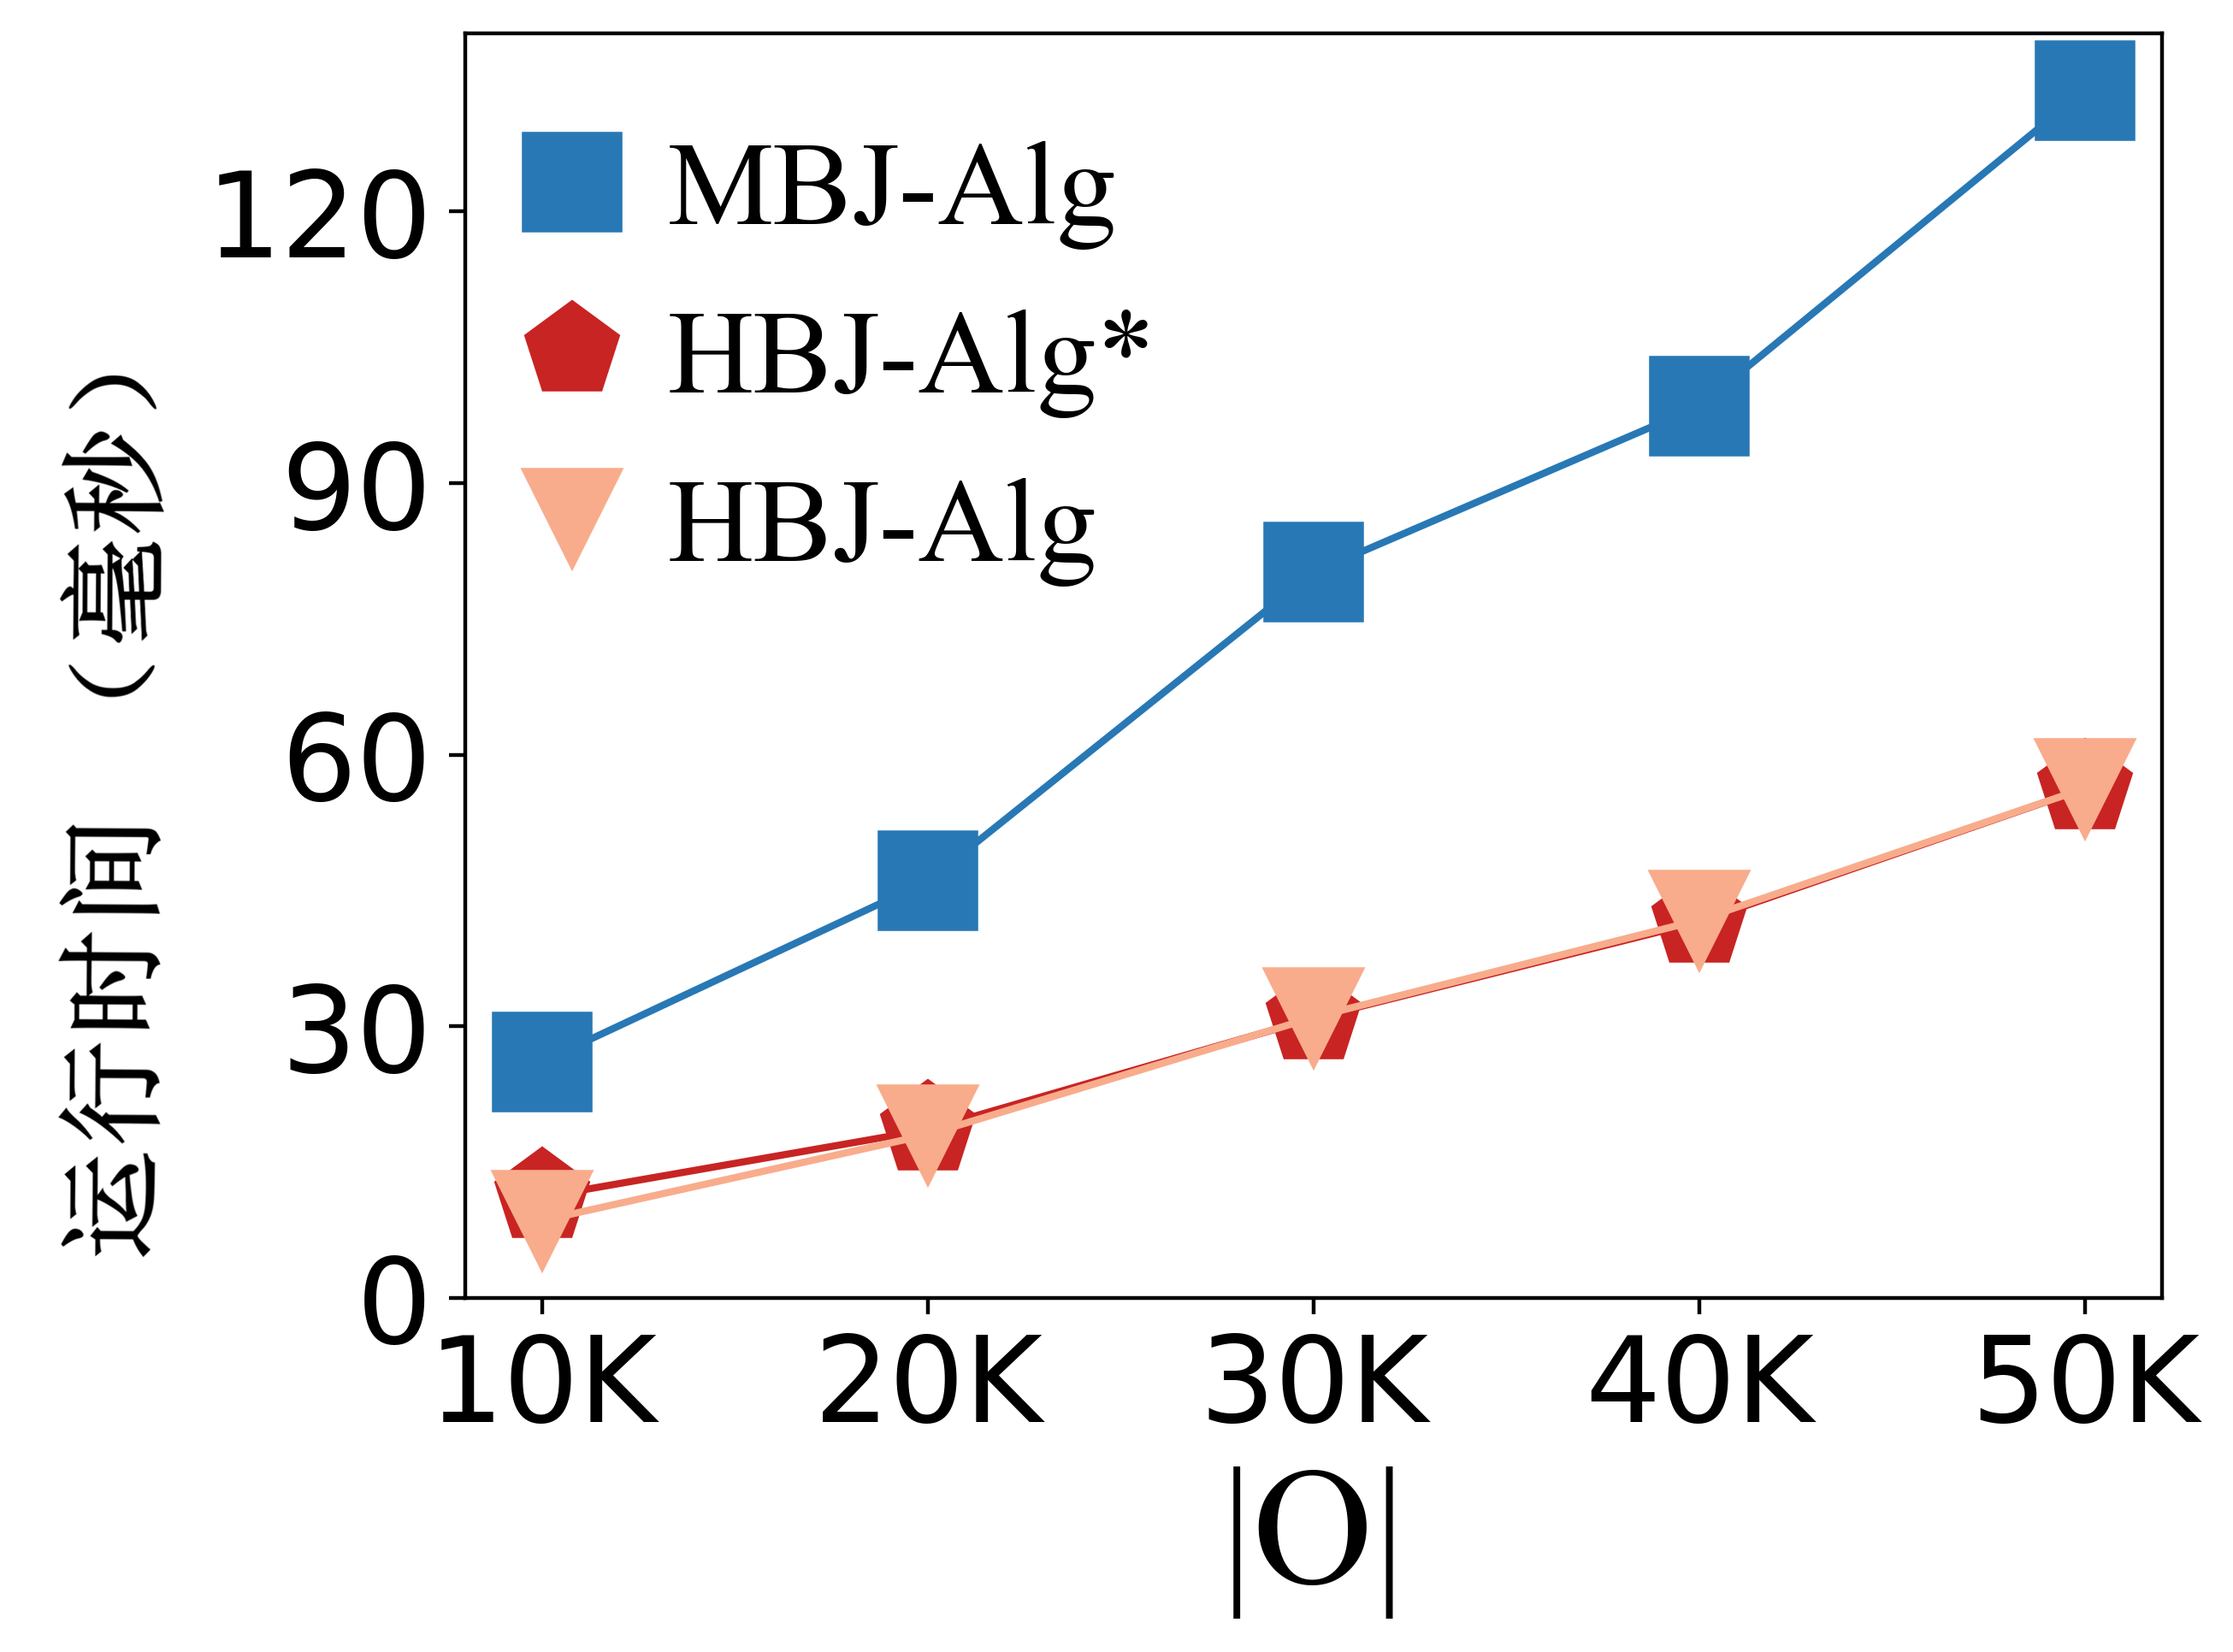
\includegraphics[width=0.5\textwidth]{fig/section6/pt-num-ctime.png}
    \label{pt-num-ctime}
}% 
\caption{不同 $|O|$ 下的构建时间影响 \subref{geo-num-ctime}:Geolife数据集下的实验; \subref{pt-num-ctime}:Porto数据集下的实验}
\label{img:vary_num_ctime}
\end{figure}

\begin{figure}[tb]
    \centering
    \subfloat[]{
    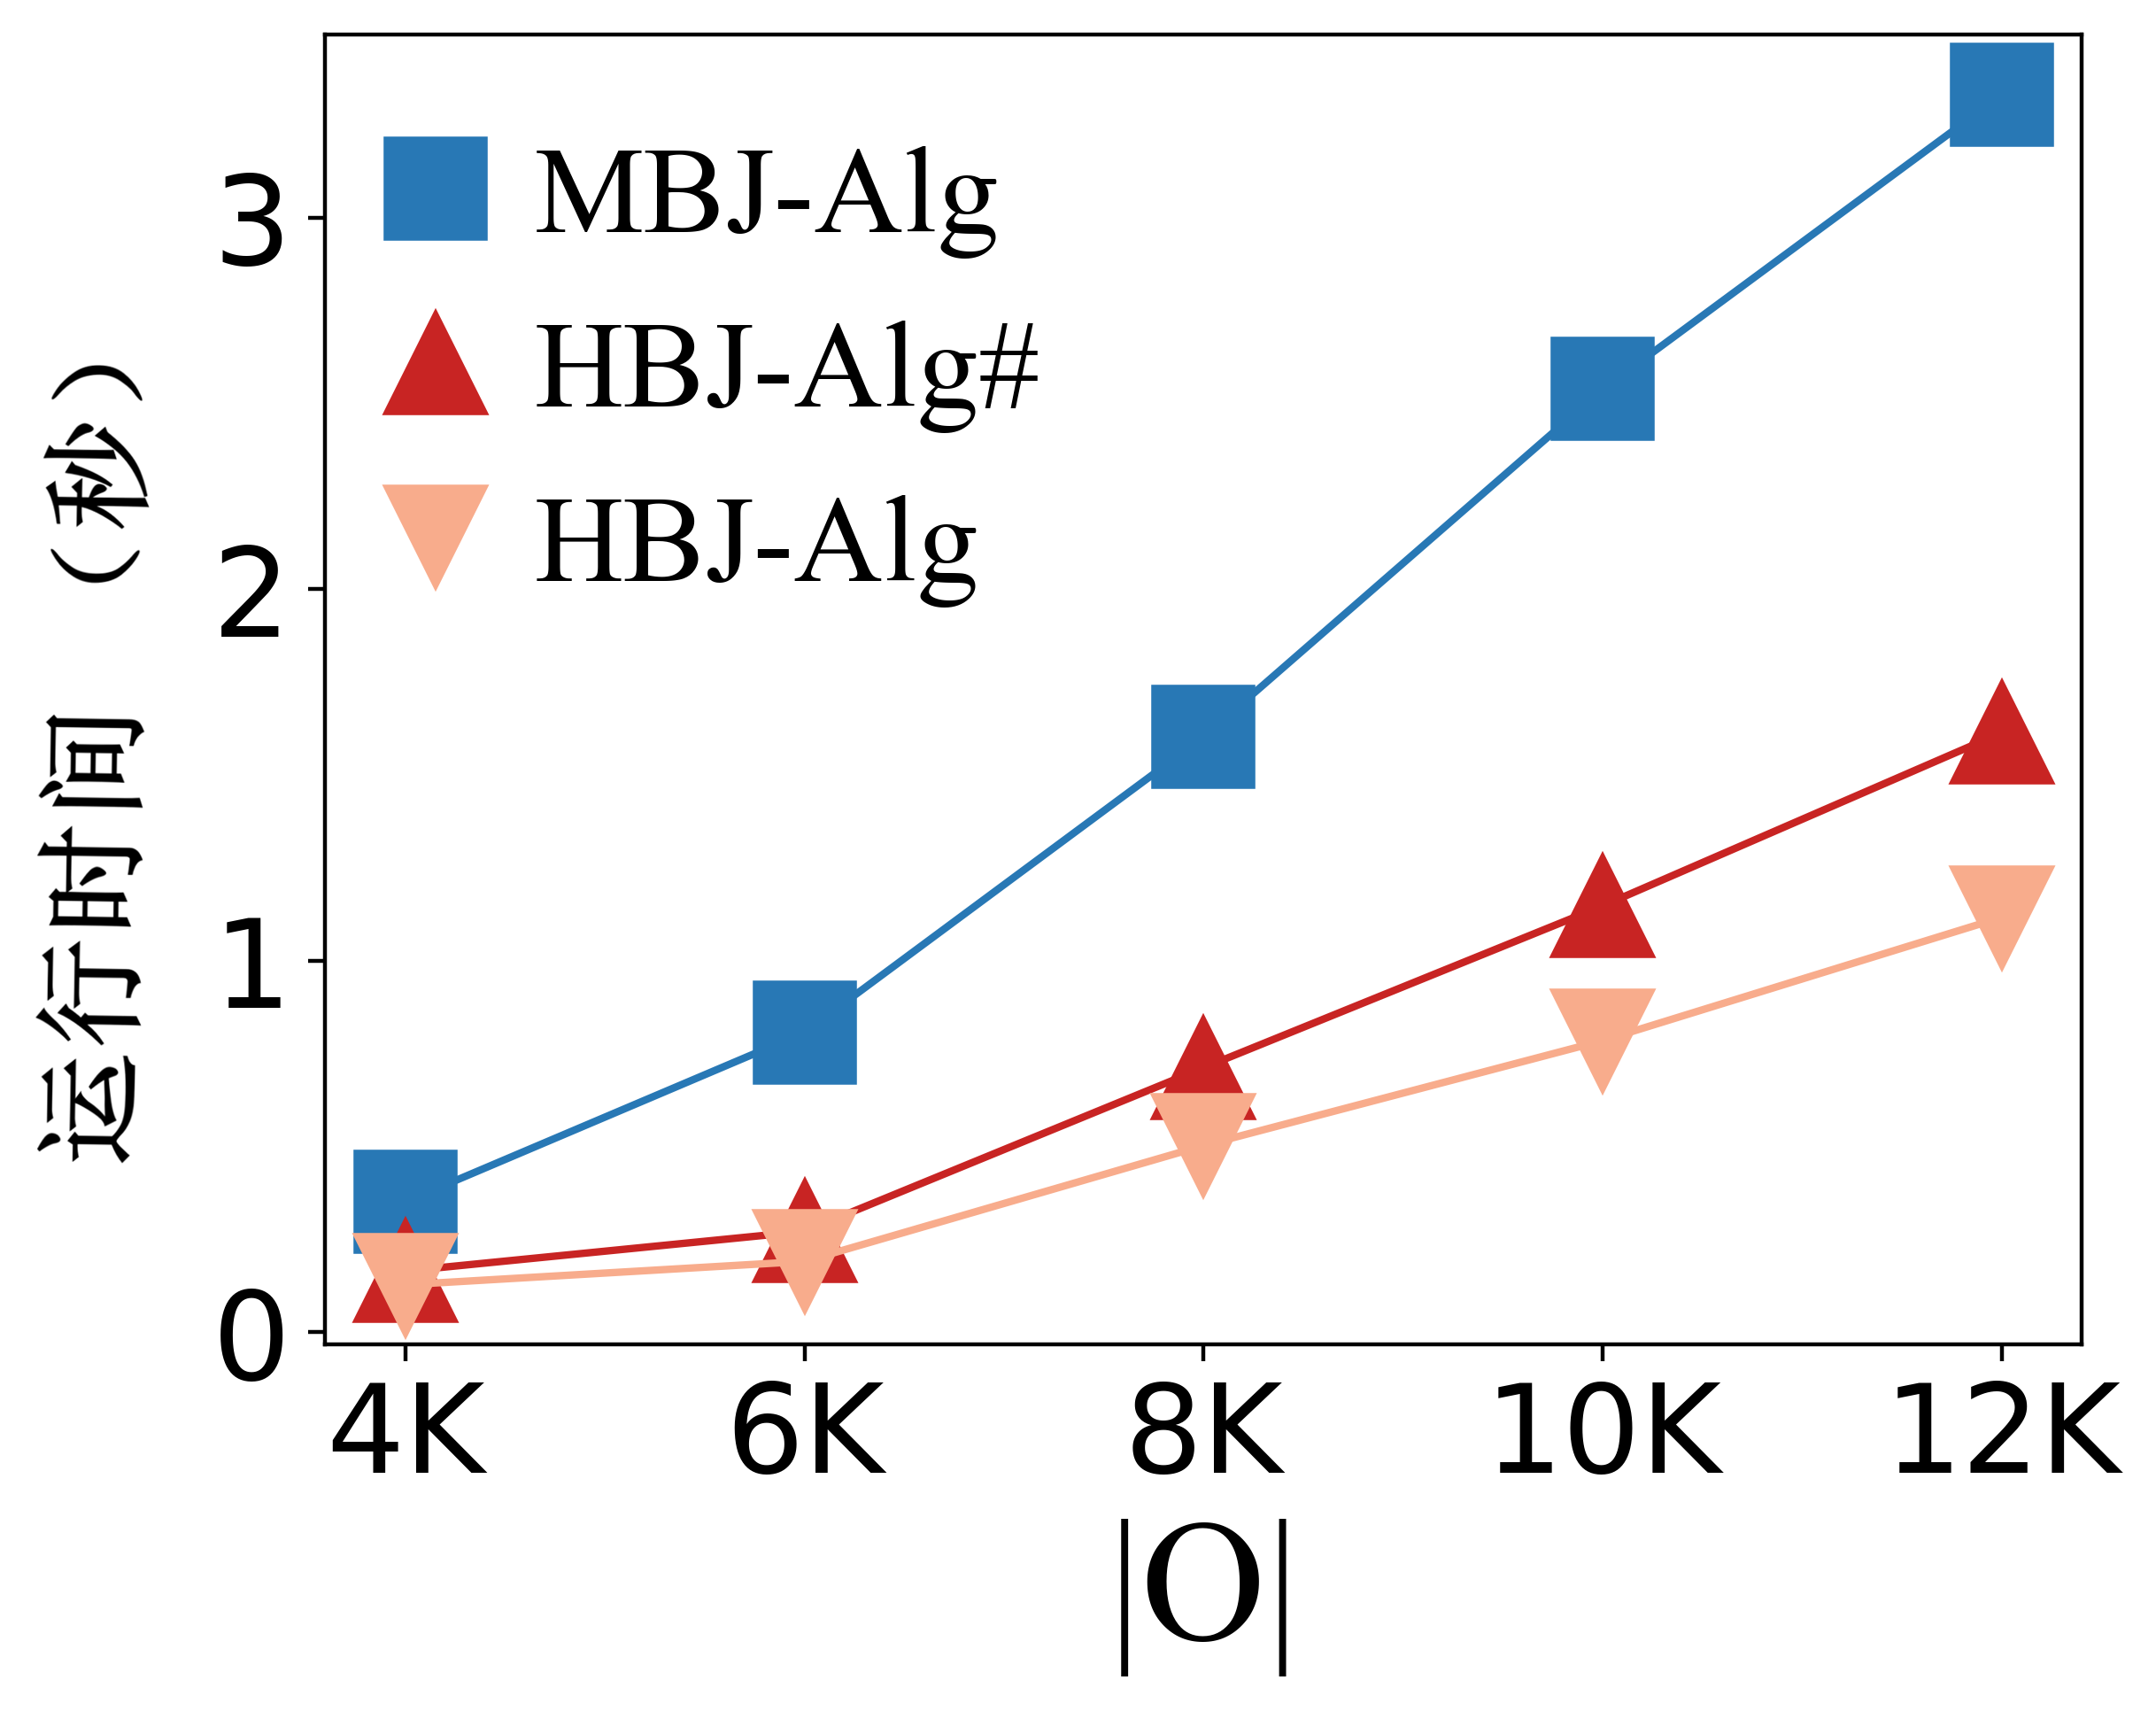
\includegraphics[width=0.5\textwidth]{fig/section6/geo-num-ftime.png}
    \label{geo-num-ftime}
}% 
\subfloat[]{
    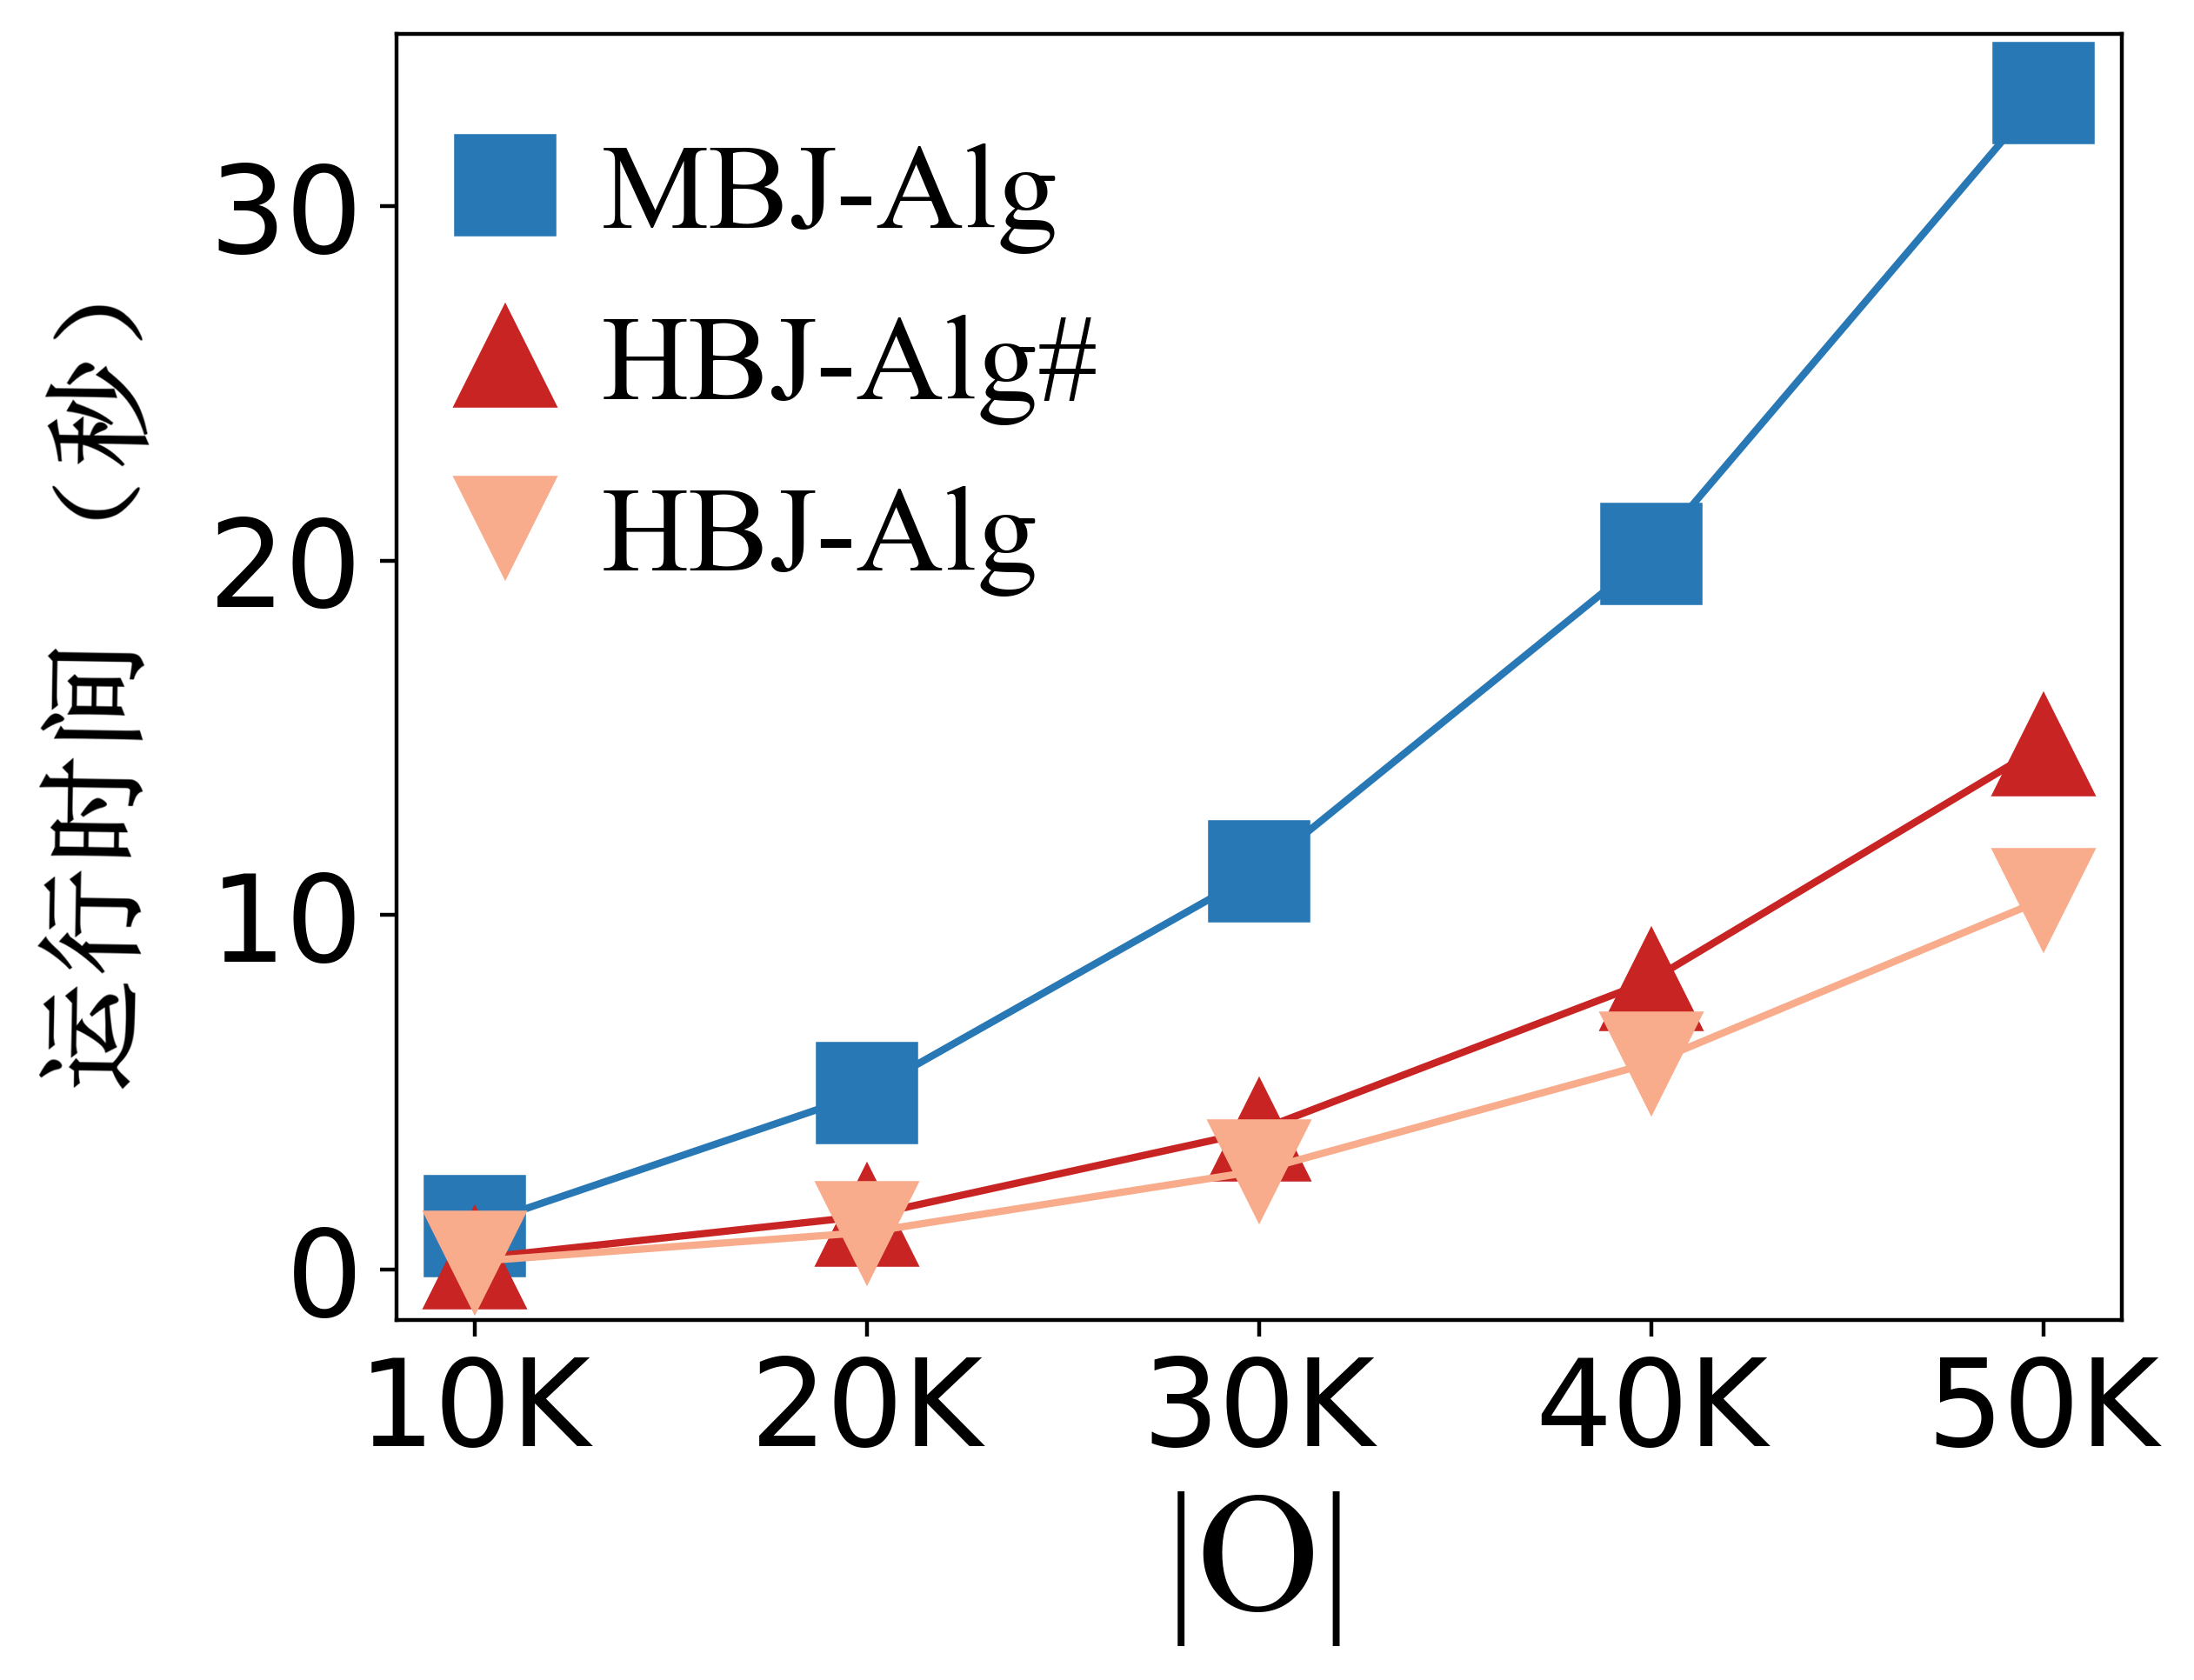
\includegraphics[width=0.5\textwidth]{fig/section6/pt-num-ftime.png}
    \label{pt-num-ftime}
}% 
\caption{不同 $|O|$ 下的查询时间影响 \subref{geo-num-ftime}:Geolife数据集下的实验; \subref{pt-num-ftime}:Porto数据集下的实验}
\label{img:vary_num_ftime}
\end{figure}

\subsubsection{特征数量的影响}
在实验中，我们将运动范围的特征集合设定为兴趣点（POI）。直观而言，在相同的时间区间运动范围内，较大的 $|\mathcal{F}|$ 意味着两个对象之间存在更多潜在的交集位置，这可能由于需要进行额外的位置检查而导致运行时间增加。如图~\ref{img:vary_poi_ftime} 所示，随着 $|\mathcal{F}|$ 的增大，所有算法的运行时间均呈现出轻微的上升趋势。然而，所提出的预检查策略和剪枝增强方法能够在早期阶段有效地剔除大量不可能满足条件的对象对，从而显著减少需要进行 POI 交集计算的候选数量。因此，POI 集合规模对整体运行时间的影响较小，进一步验证了所提出方法的良好可扩展性。

\begin{figure}[tb]
    \centering
    \subfloat[]{
    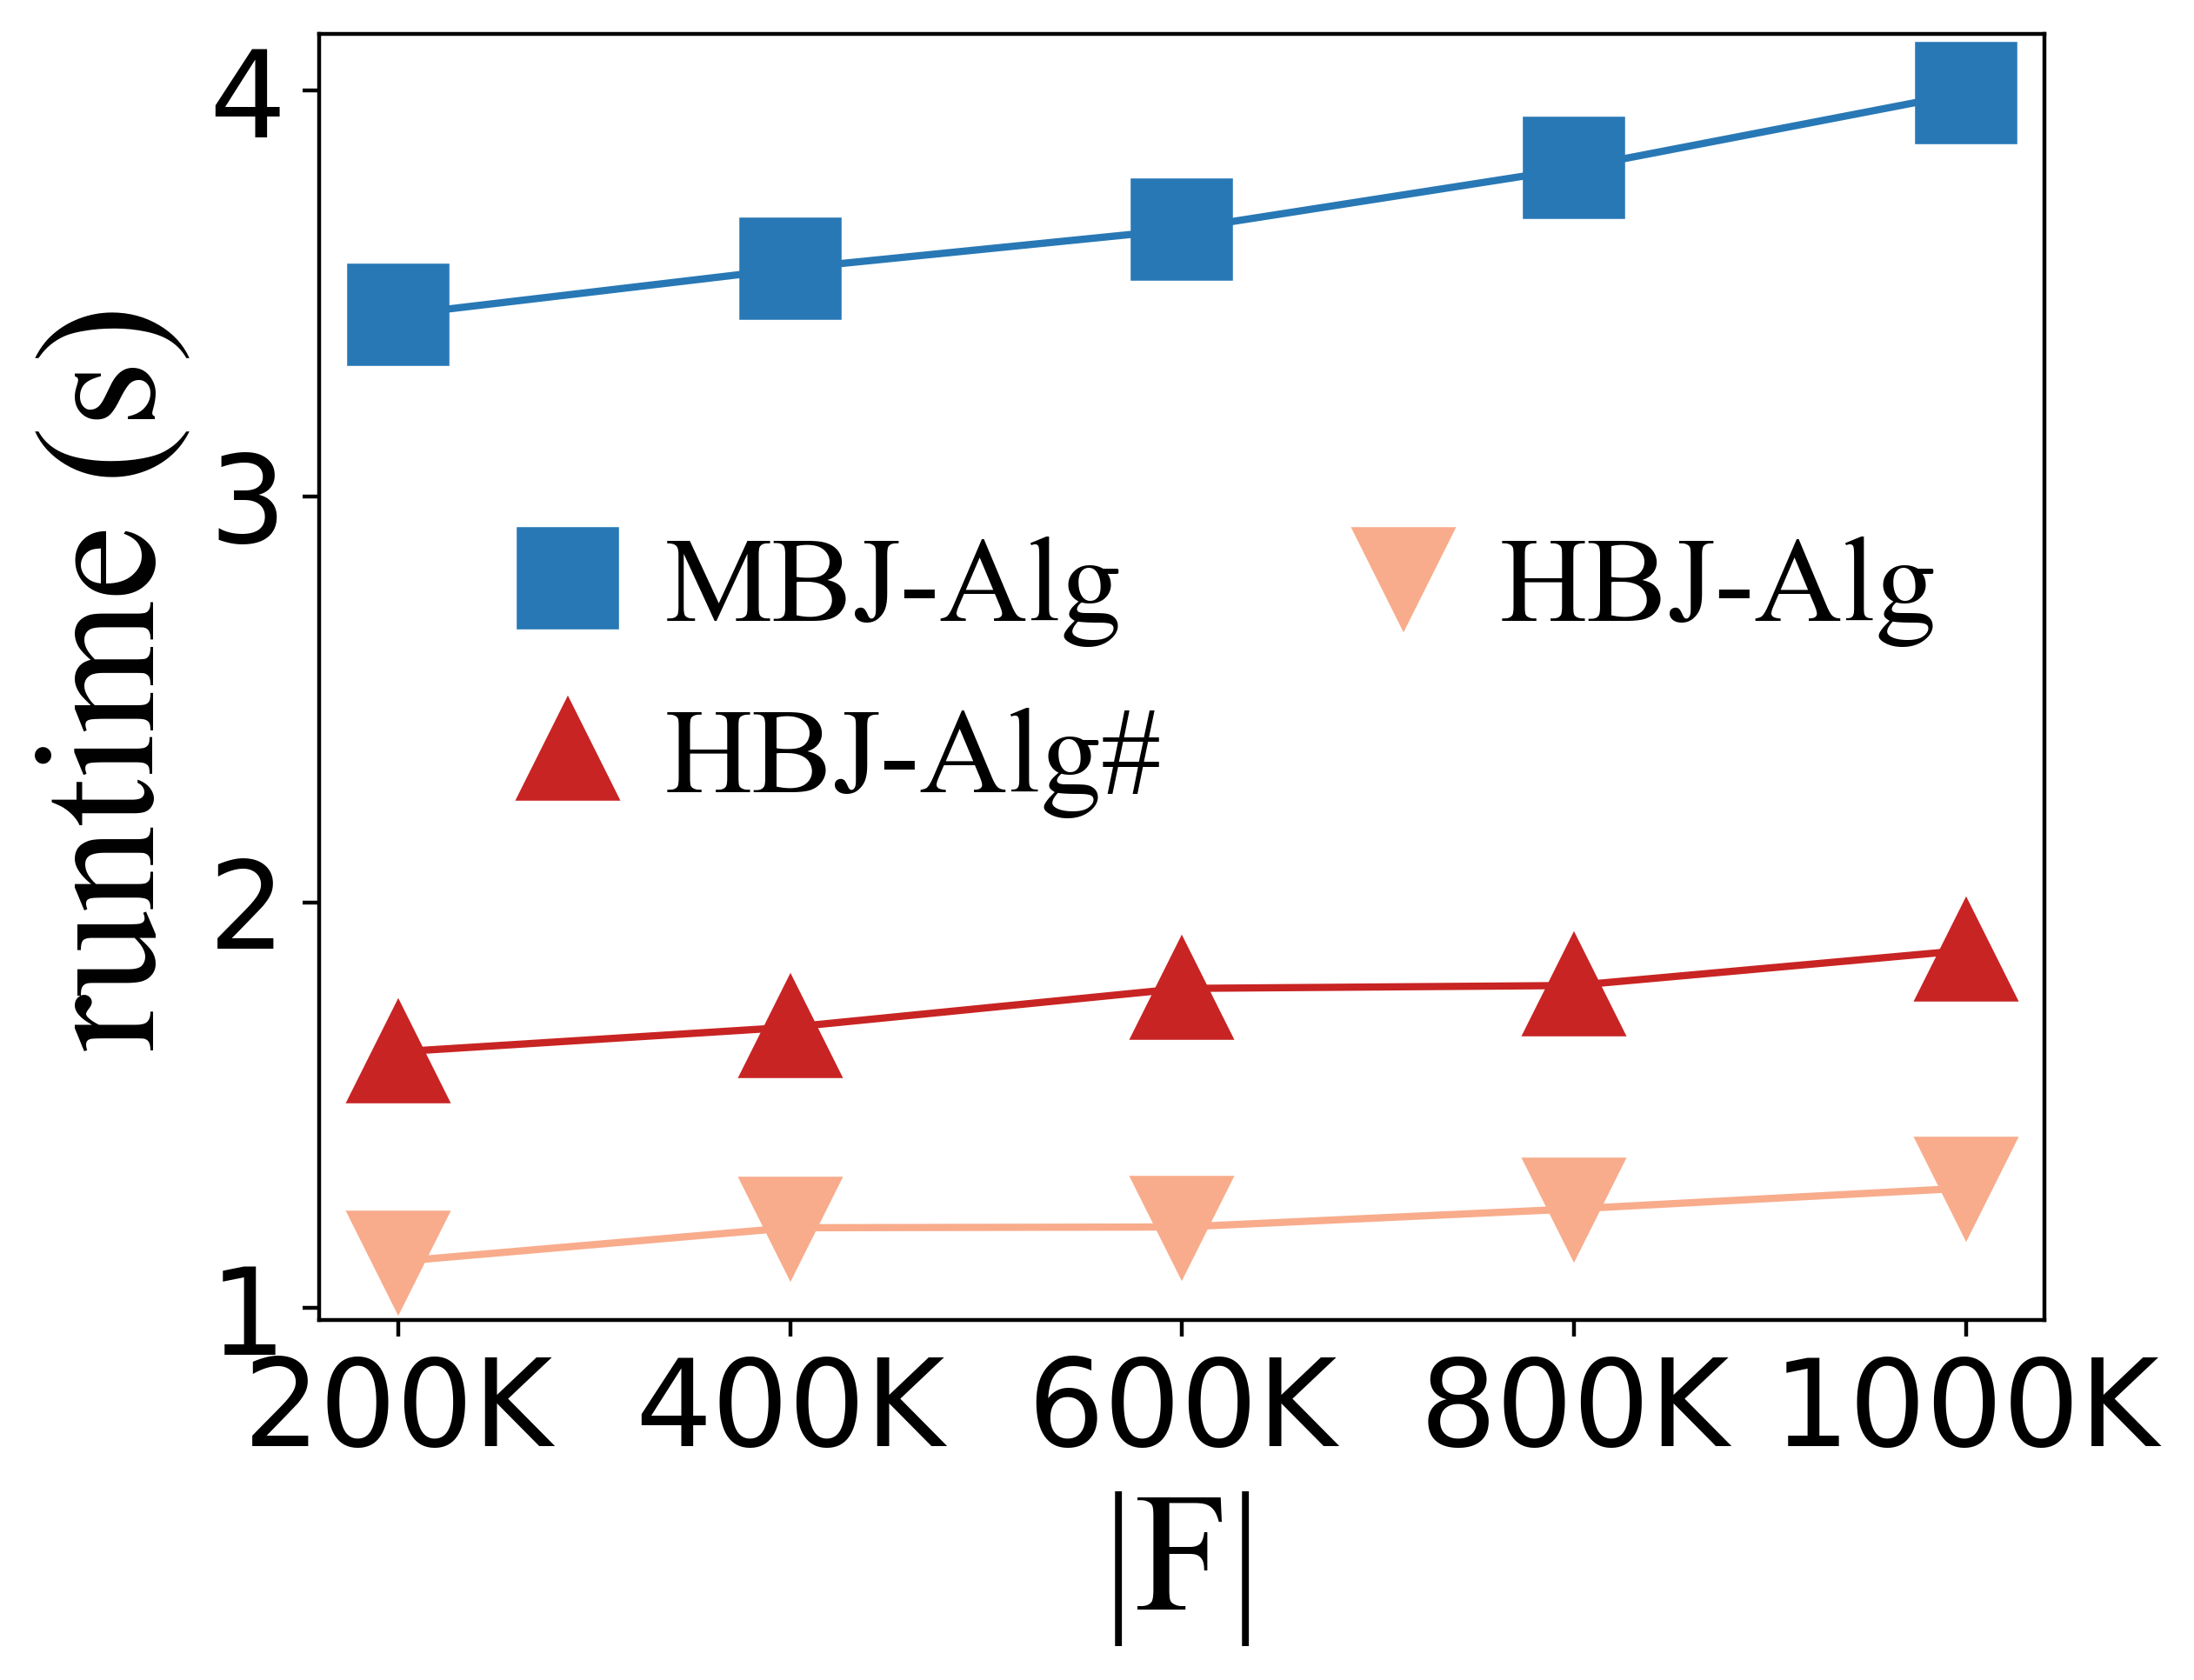
\includegraphics[width=0.5\textwidth]{fig/section6/geo-poi-ftime.png}
    \label{geo-poi-ftime}
}% 
 \subfloat[]{
    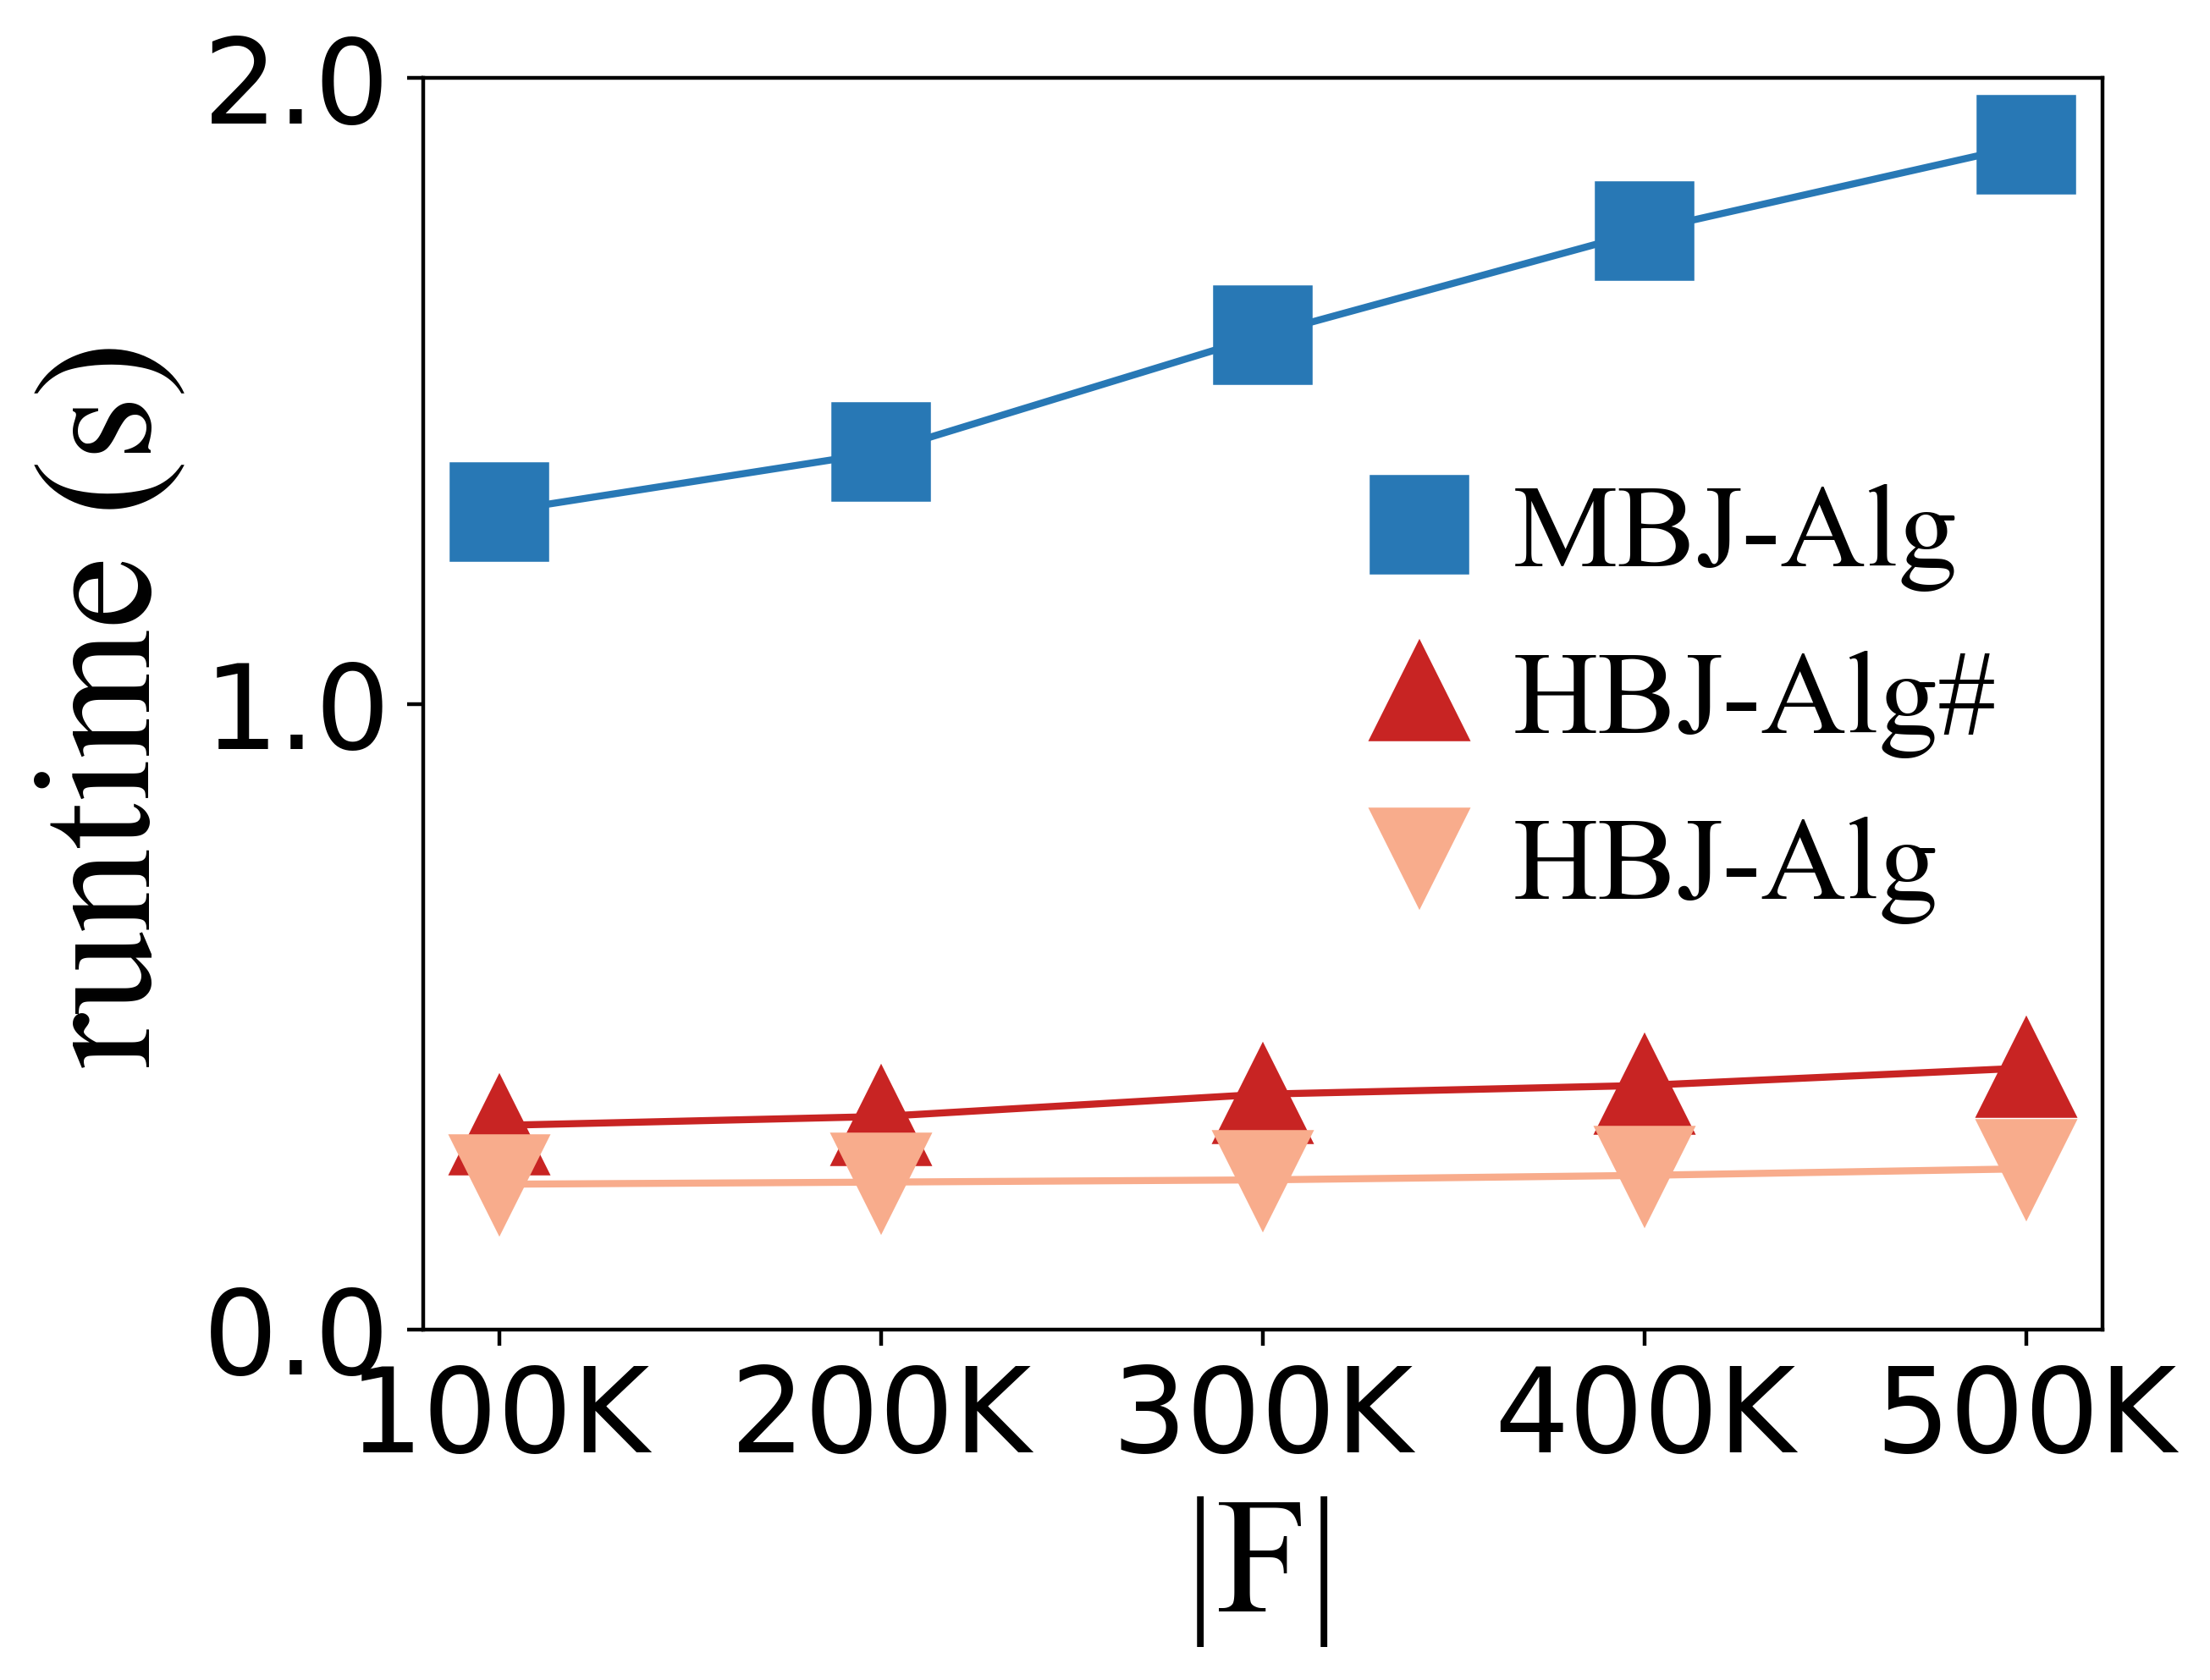
\includegraphics[width=0.5\textwidth]{fig/section6/pt-poi-ftime.png}
    \label{pt-poi-ftime}
}% 
\caption{POI 数量对运行时间的影响 \subref{geo-poi-ftime}:Geolife数据集下的实验; \subref{pt-poi-ftime}:Porto数据集下的实验}
\label{img:vary_poi_ftime}
\end{figure}

\subsubsection{时间区间的影响}
我们使用 $|I|$ 表示给定时间区间的持续时长。具体而言，在 Geolife 数据集中，$|I|$ 从 10 秒变化到 50 秒；在 Porto 数据集中，$|I|$ 从 15 秒变化到 75 秒。较大的 $|I|$ 会扩大潜在的时间区间运动范围，从而导致具有交集的对象对数量增加以及候选集规模增大。因此，所有算法在识别满足条件的对象对时都需要更多的计算开销。图~\ref{img:vary_I_ftime} 展示了随着 $|I|$ 增大时的效率表现。正如预期的那样，随着 $|I|$ 的增加，所有算法的运行时间均呈上升趋势，其中 HBJ-Alg 在所有参数设置下始终优于 MBJ-Alg 和 HBJ-Alg\#。通过利用 M*-tree，我们在一定程度上提升了过滤性能，并减少了后续需要进一步处理的候选对象数量。然而，由于 M-tree 的原始设计在构建阶段需要进行耗时的节点分裂操作，其并不适合直接用于 IS-Join 查询。此外，在大规模移动对象场景下，对仅覆盖单个时间区间运动范围的圆进行索引，可能会导致搜索空间膨胀，从而对查询性能产生不利影响。

\begin{figure}[tb]
    \centering
    \subfloat[]{
    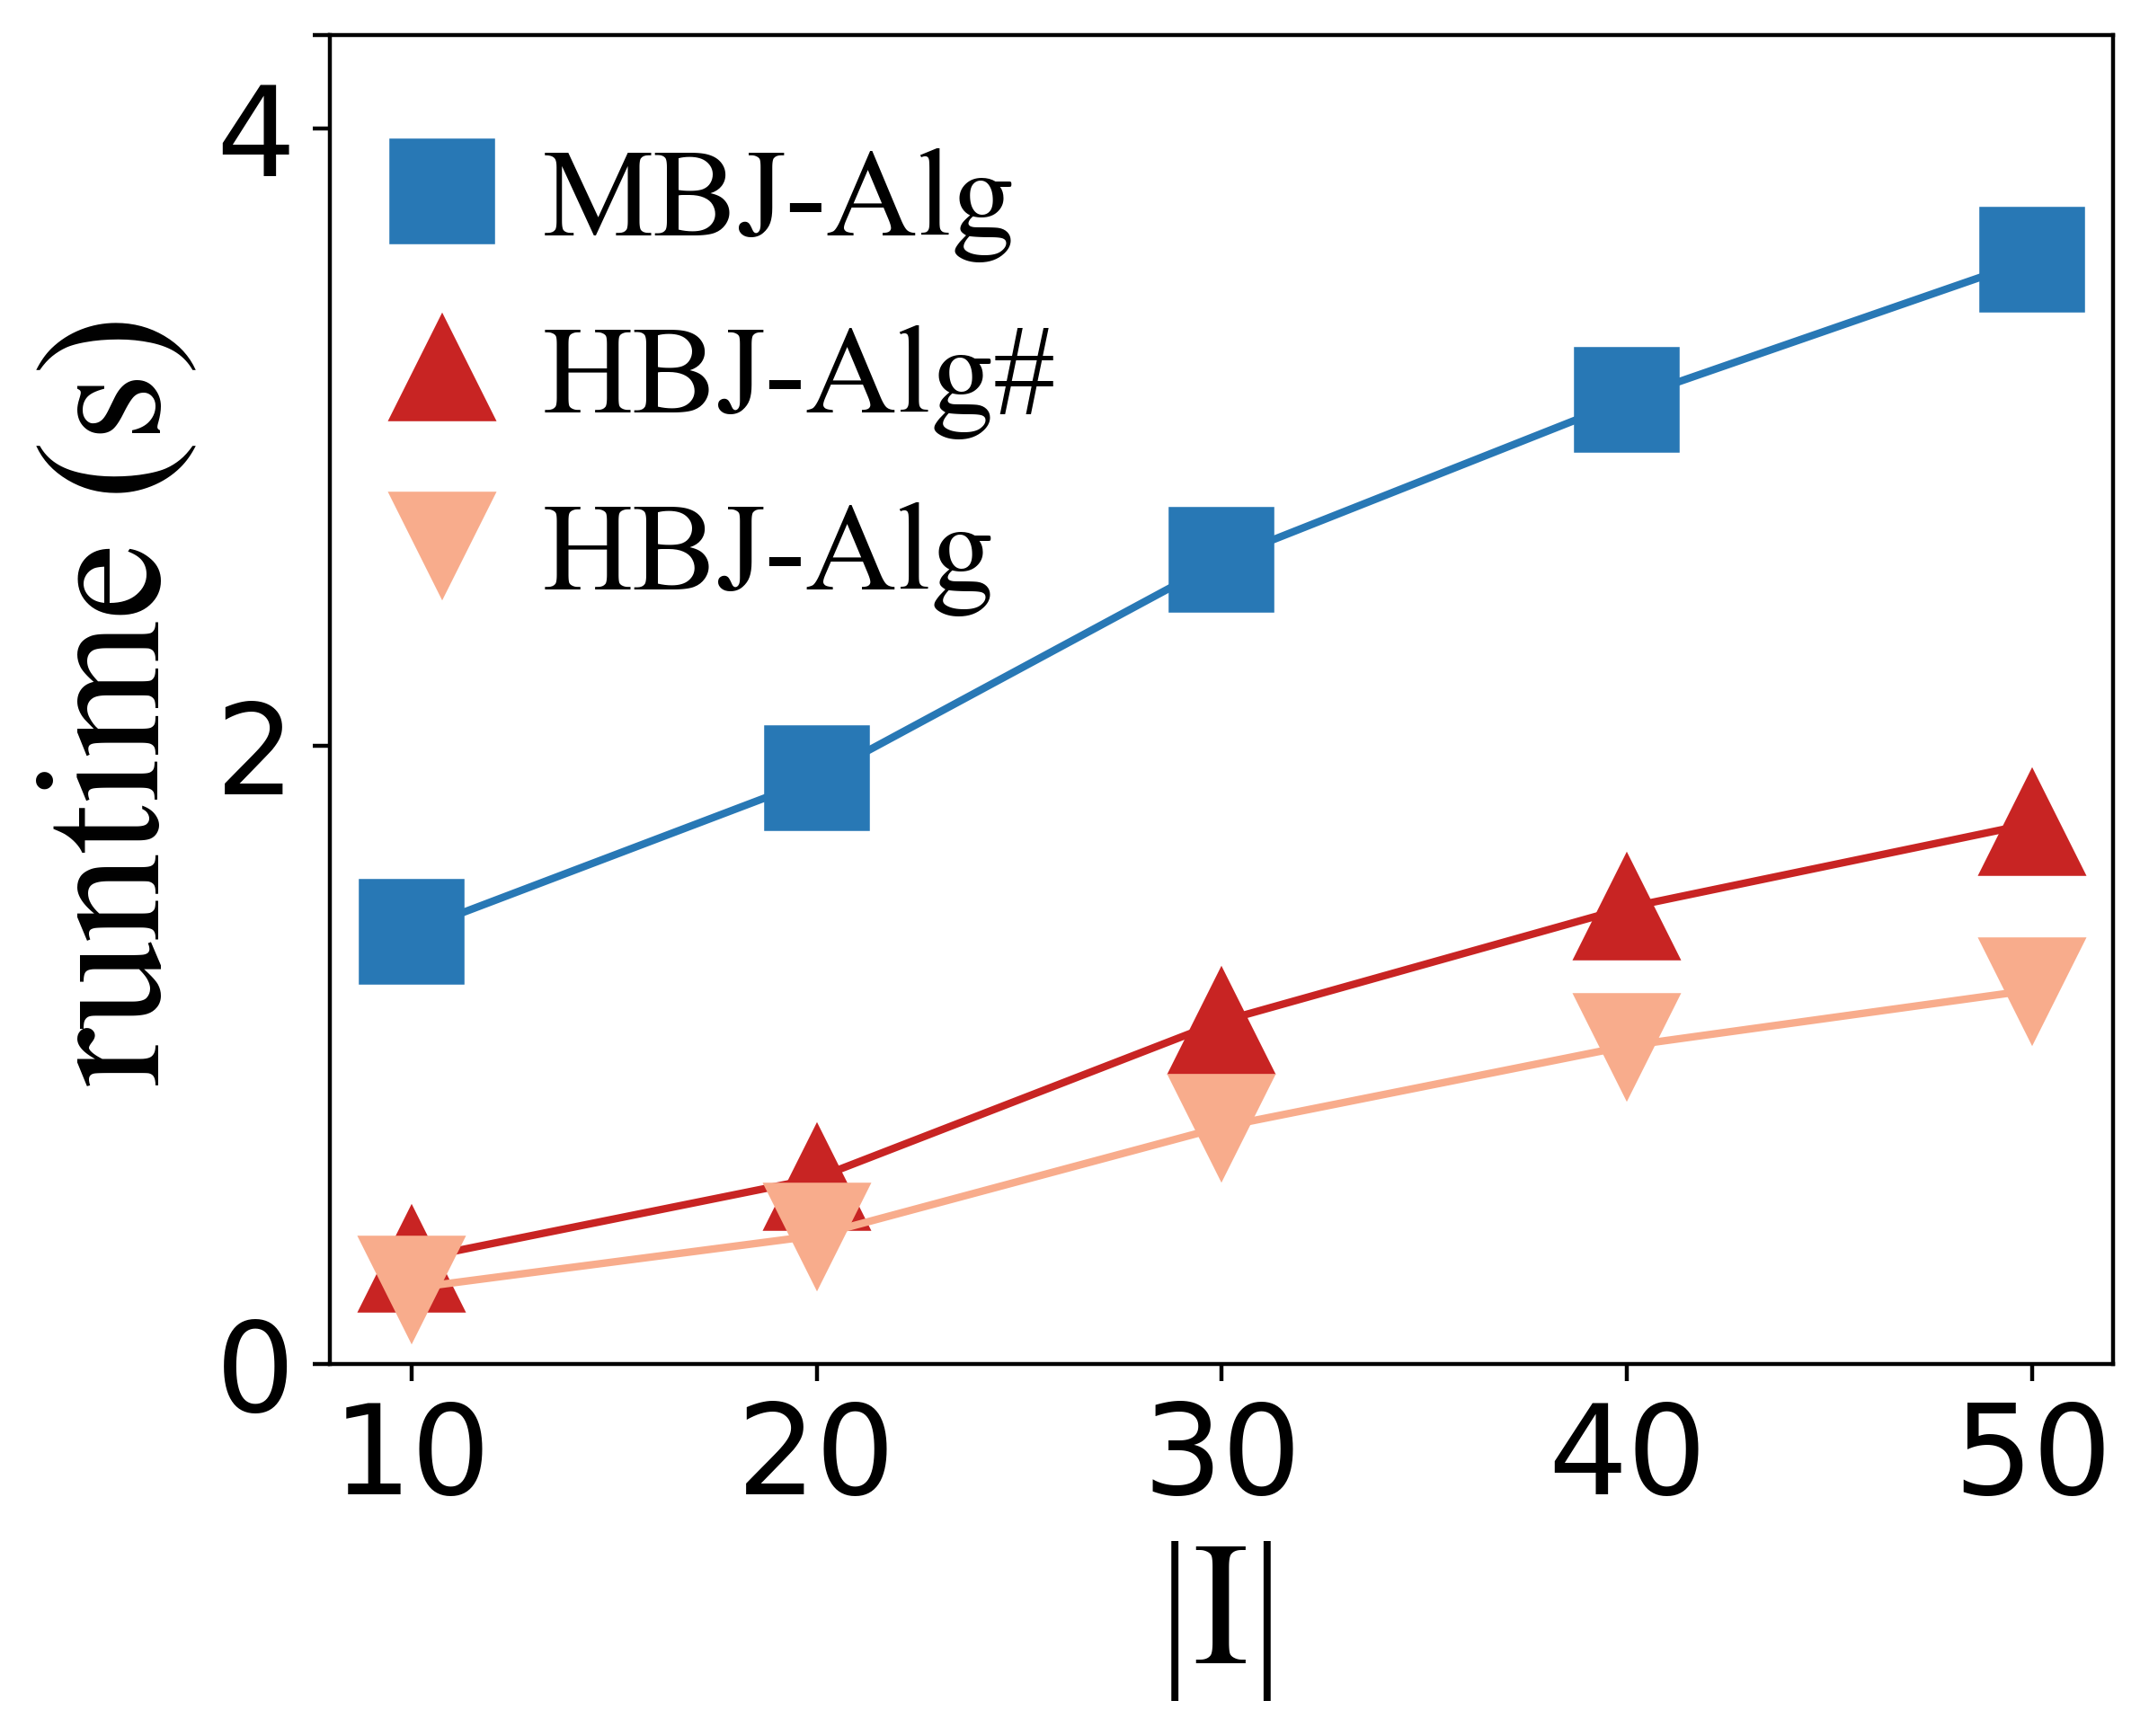
\includegraphics[width=0.4\textwidth]{fig/section6/geo-I-ftime.png}
    \label{geo-I-ftime}
}% 
\hfill
 \subfloat[]{
    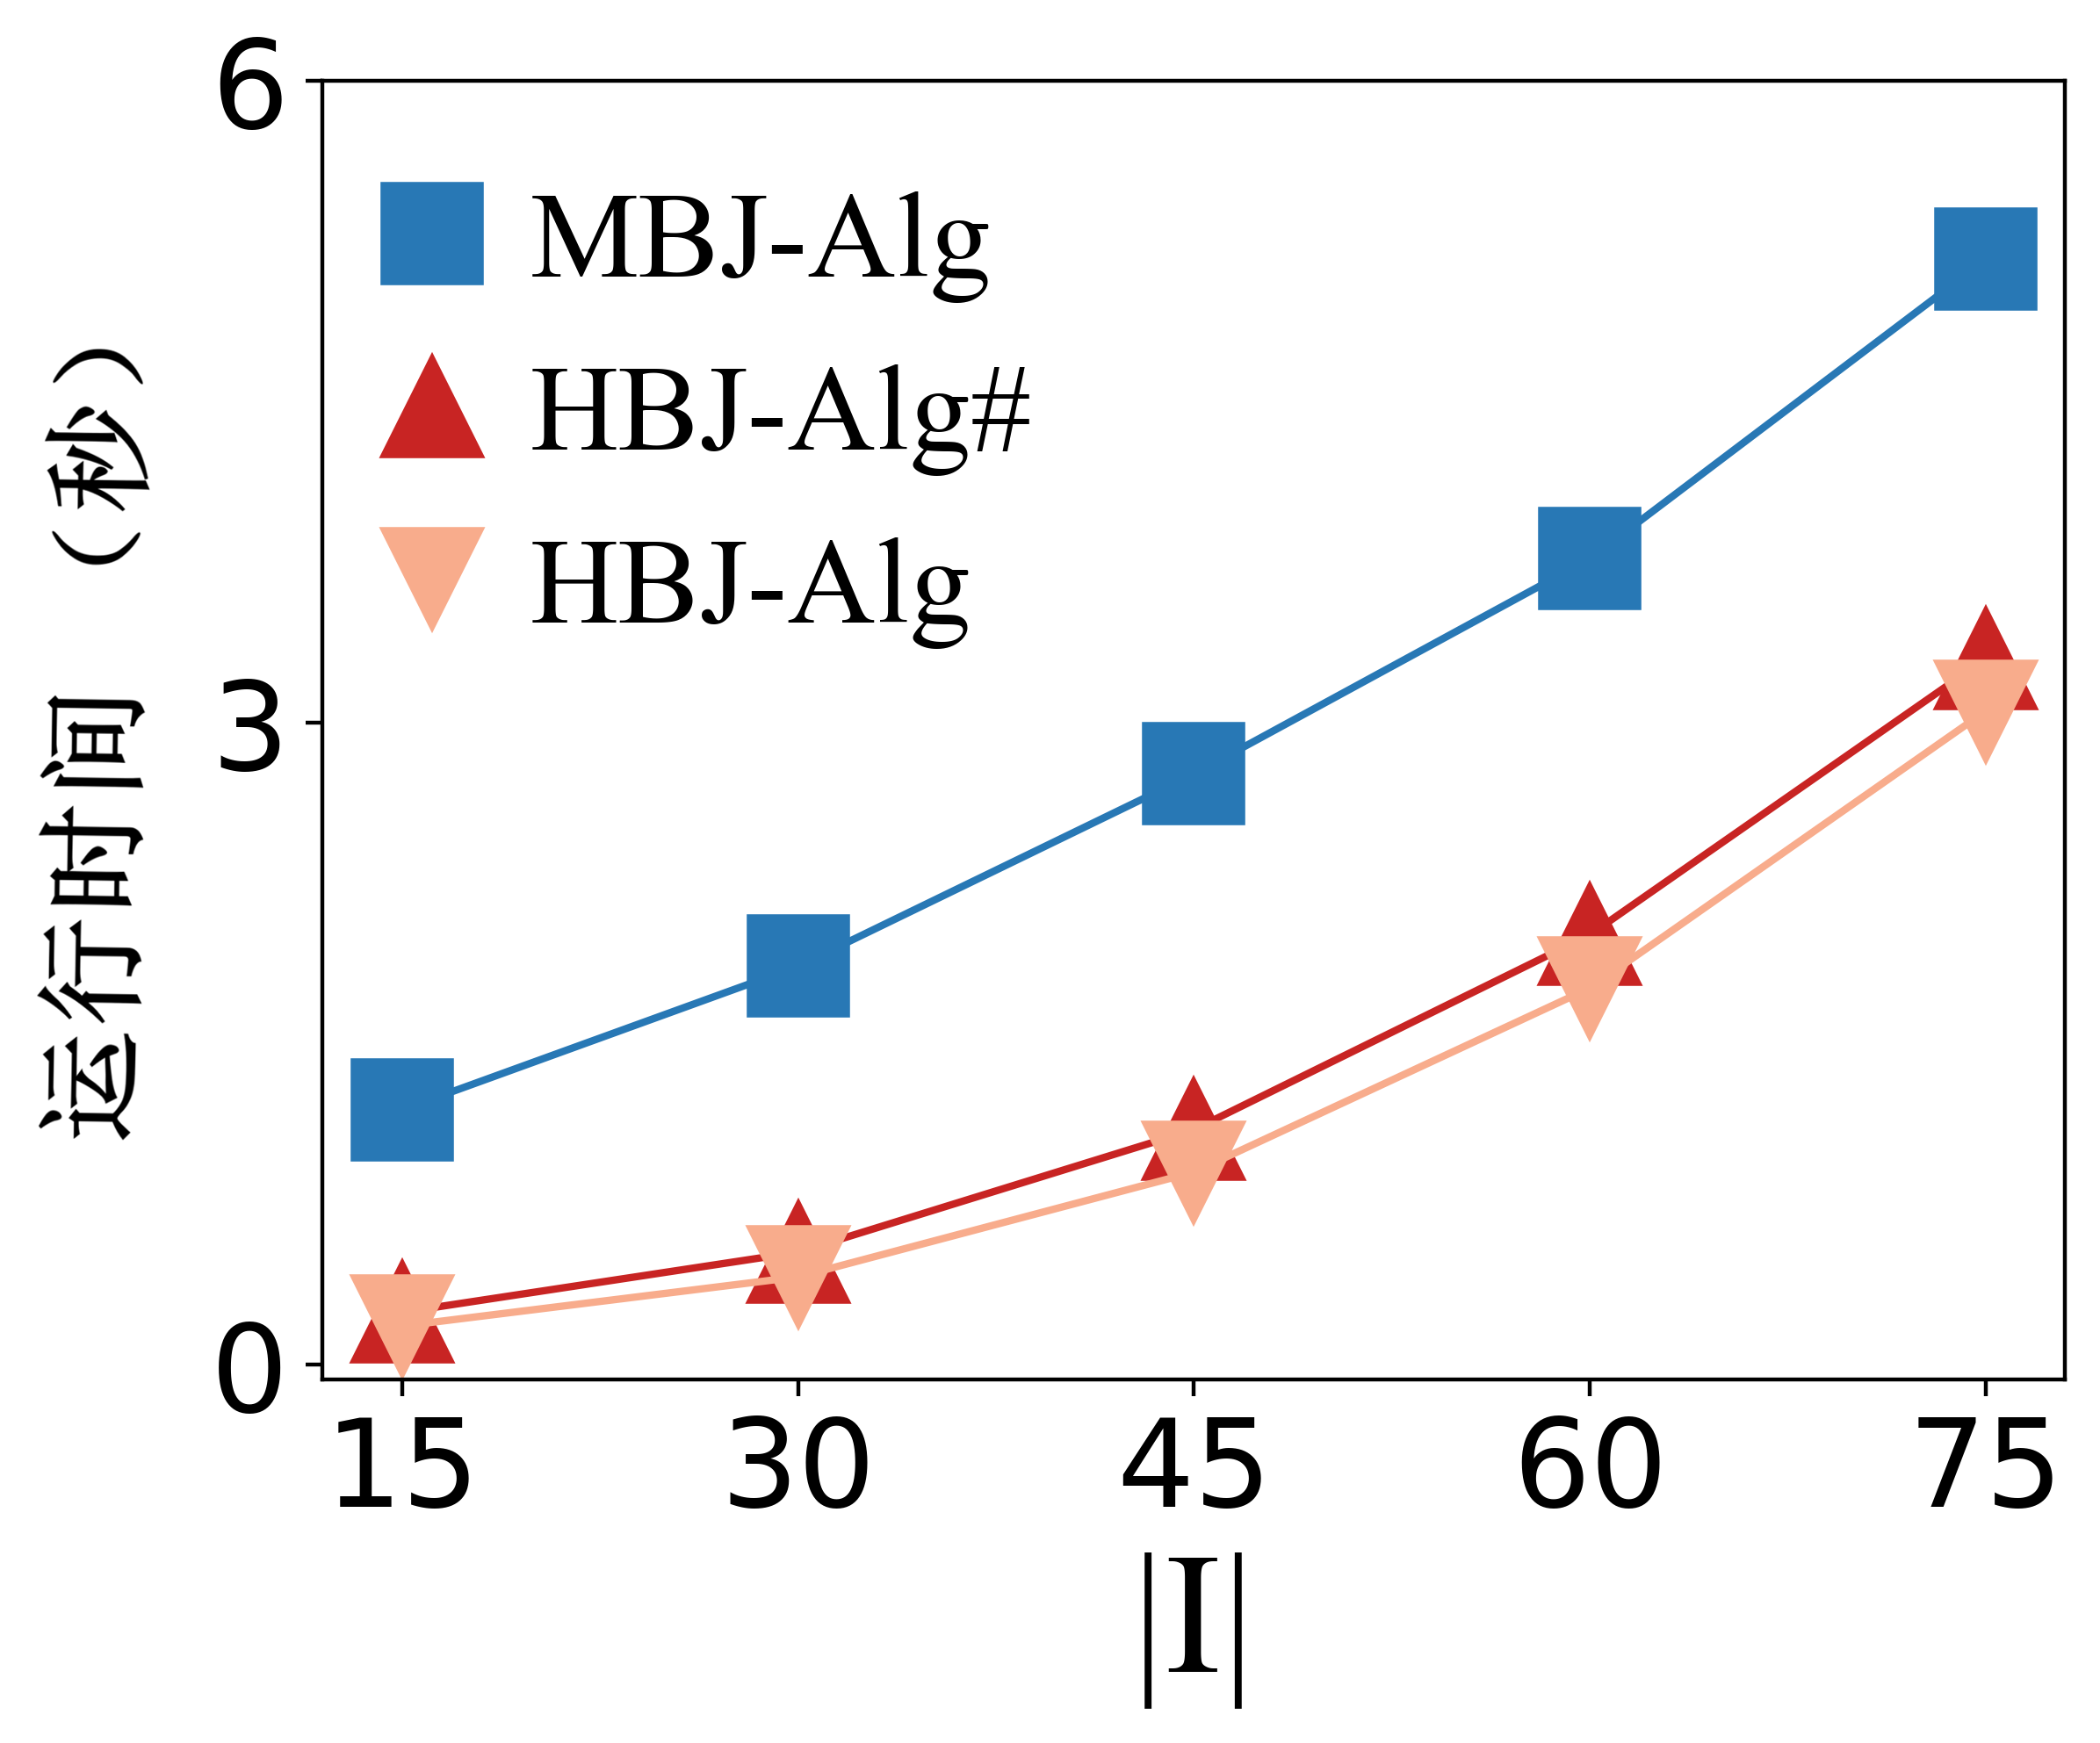
\includegraphics[width=0.4\textwidth]{fig/section6/pt-I-ftime.png}
    \label{pt-I-ftime}
}% 
\caption{$|I|$ 对运行时间的影响 \subref{geo-I-ftime}:Geolife数据集下的实验; \subref{pt-I-ftime}:Porto数据集下的实验}
\label{img:vary_I_ftime}
\end{figure}

\subsubsection{$\epsilon$ 的影响}

较小的 $\epsilon$ 值意味着需要探测更多的时间点运动范围，使得放松后的相似度更加接近真实的交集相似度，从而带来更高的计算开销，并导致运行时间的增加。图~\ref{img:vary_ep_ftime} 展示了在变化放松参数 $\epsilon$ 时的效率表现。在实验中，我们将时间点运动范围的数量从 2 变化到 10。随着 $\epsilon$ 的变化，可以观察到运行时间呈现出轻微的上升趋势。同时也可以看到，在所有参数设置下，HBJ-Alg 始终表现出最优的性能。

\begin{figure}[tb]
    \centering
    \subfloat[]{
    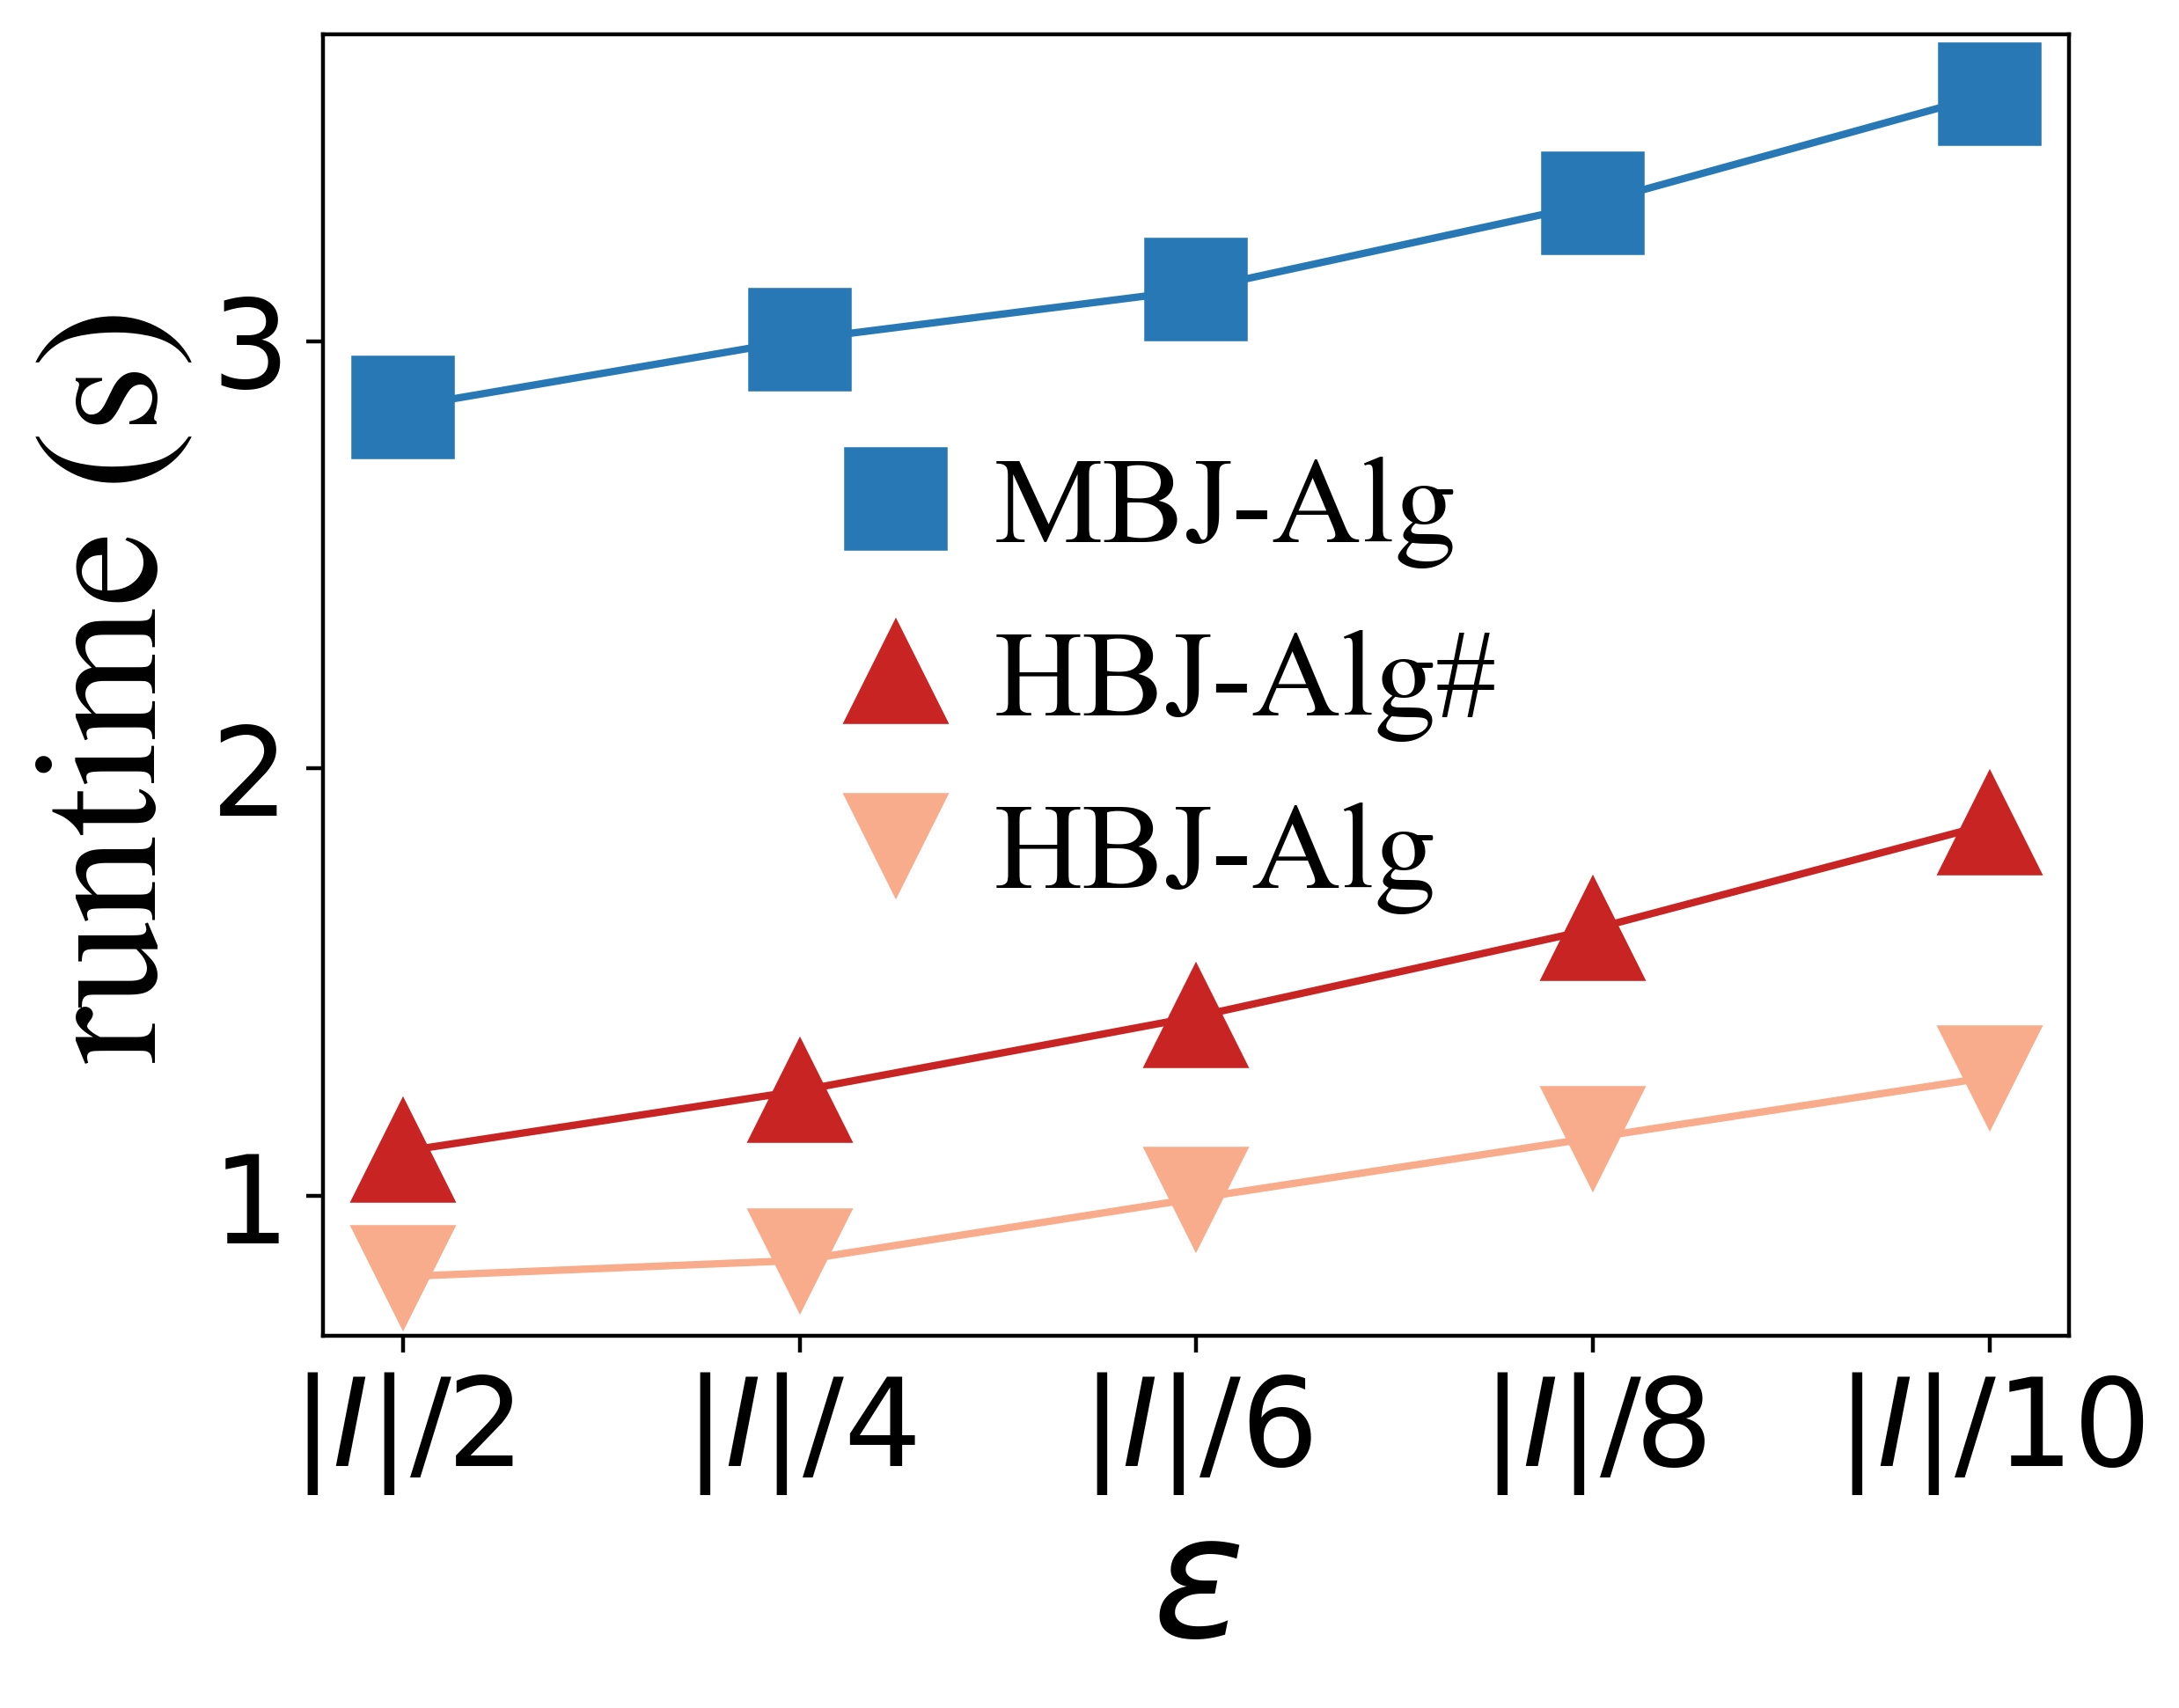
\includegraphics[width=0.4\textwidth]{fig/section6/geo-ep-ftime.png}
    \label{geo-ep-ftime}
}% 
\hfill
 \subfloat[]{
    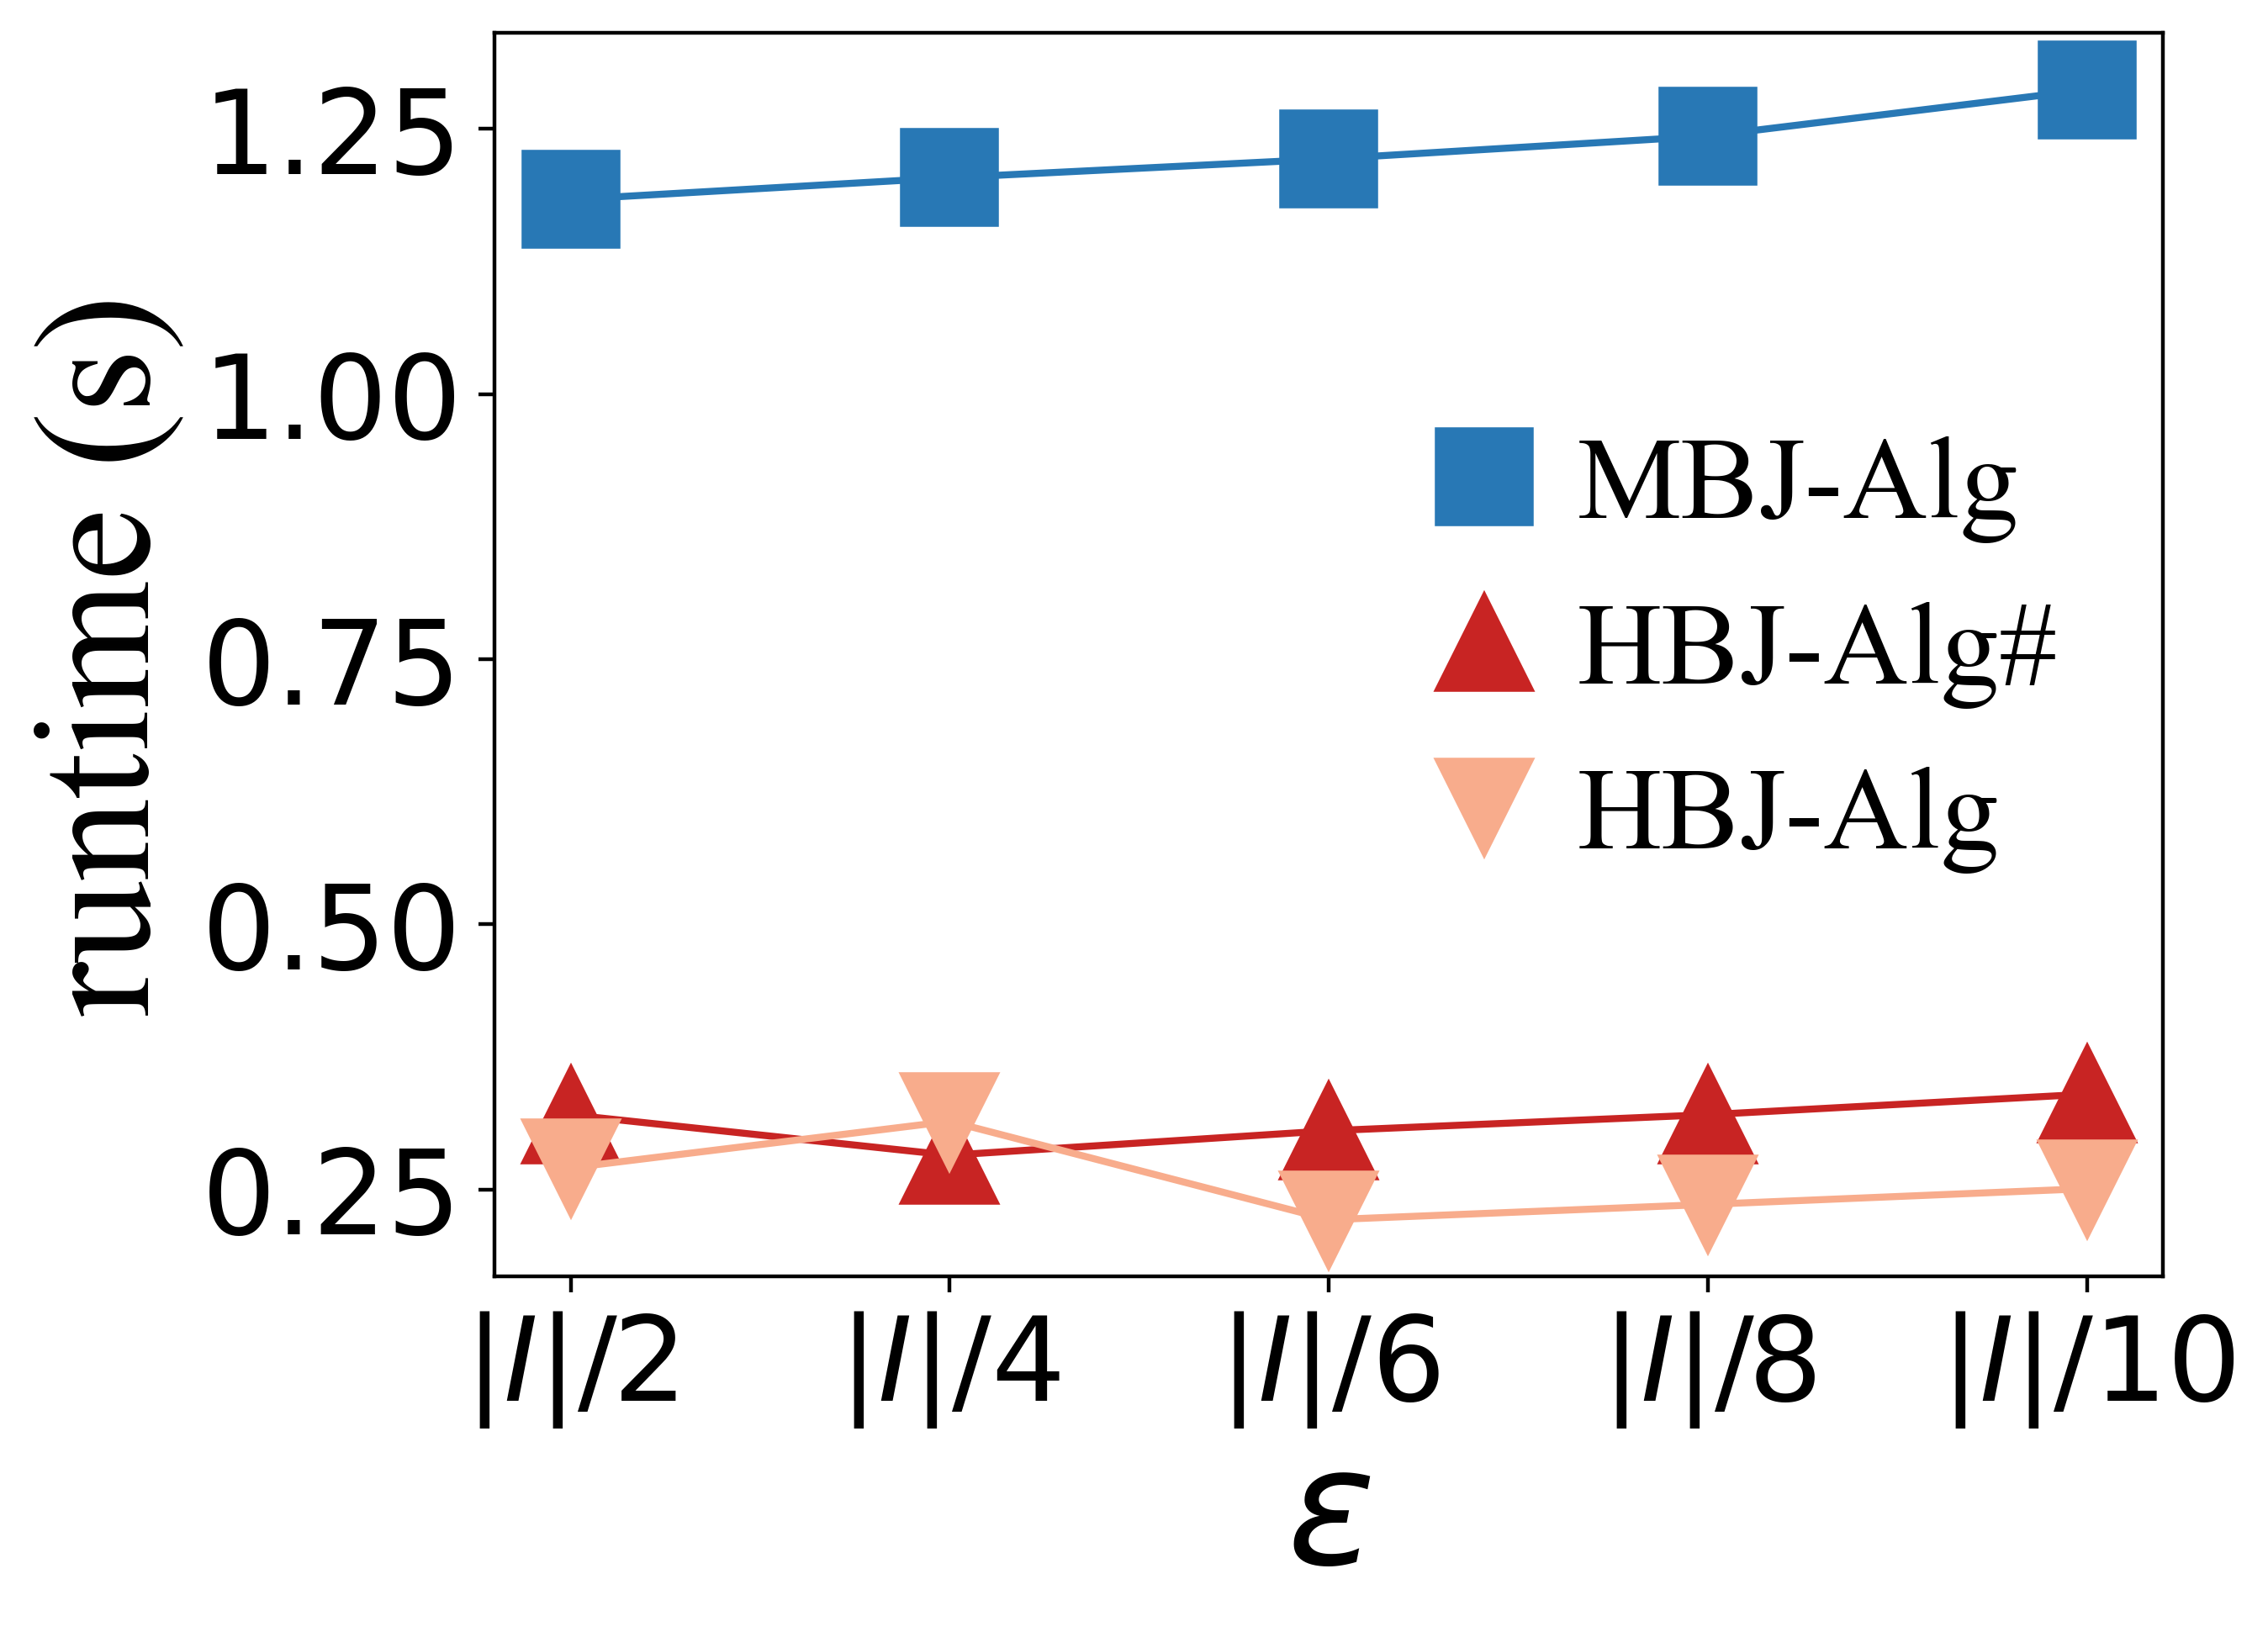
\includegraphics[width=0.4\textwidth]{fig/section6/pt-ep-ftime.png}
    \label{pt-ep-ftime}
}% 
\caption{参数 $\epsilon$ 的影响 \subref{geo-ep-ftime}:Geolife数据集下的实验; \subref{pt-ep-ftime}:Porto数据集下的实验}
\label{img:vary_ep_ftime}
\end{figure}




\section{基于 M*-树的连接算法}
\label{sec:baseLine}

\begin{algorithm}[!h]
    \caption{基于基本过滤与精炼的算法}
    \label{alg:bf-alg}
    
    \Input{
    两个移动对象集合，$\mathcal{A}$ 和 $\mathcal{B}$；\newline
    交集相似度阈值，$\theta$。
    }
    \Output{
    交集对，$\mathcal{R}$。
    }
    
    \textbf{初始化:} $\mathcal{L} \leftarrow \emptyset$；
    
    \For(\tcc*[f]{遍历集合 $\mathcal{A}$}){$o \in \mathcal{A}$}{
        \For(\tcc*[f]{遍历集合 $\mathcal{B}$}){$o' \in \mathcal{B}$}{
            \If{$dist(MR(o), MR(o')) \leq MR(o).a + MR(o').a$}{
                $\mathcal{L}.add((o, o'))$；
            }
        }
    }
    
    \For(\tcc*[f]{精炼步骤}){$(o, o') \in \mathcal{L}$}{
        \If{$IS(o, o', I, \epsilon) \geq \theta$}{
            $\mathcal{R} \leftarrow \{\mathcal{R}, (o, o')\}$；
        }
    }
    
    \textbf{return} $\mathcal{R}$；
    \end{algorithm}

首先，我们介绍一种基于 M*-树的连接算法（MBJ-Alg）用于计算 IS-Join，这作为基线方法。M*-树是 M-tree 的一种扩展~\cite{DBLP:conf/sebd/CiacciaPRZ97,DBLP:conf/vldb/CiacciaPZ97}。MBJ-Alg 是一个两阶段算法，结合了预检查策略，其中使用 M-tree 的变体来增强候选对象的过滤能力。

在阶段 1 中，M*-树使用近似圆来索引时间区间内的运动范围。这种圆形索引允许提前剪枝不合格对象，从而集中于更可能发生交集的候选对象。在阶段 2 中，对候选对象在时间点运动范围级别进行评估。下面将介绍 M*-树的结构及其在 IS-Join 查询中的应用。

\begin{figure}[htbp]
    \centering
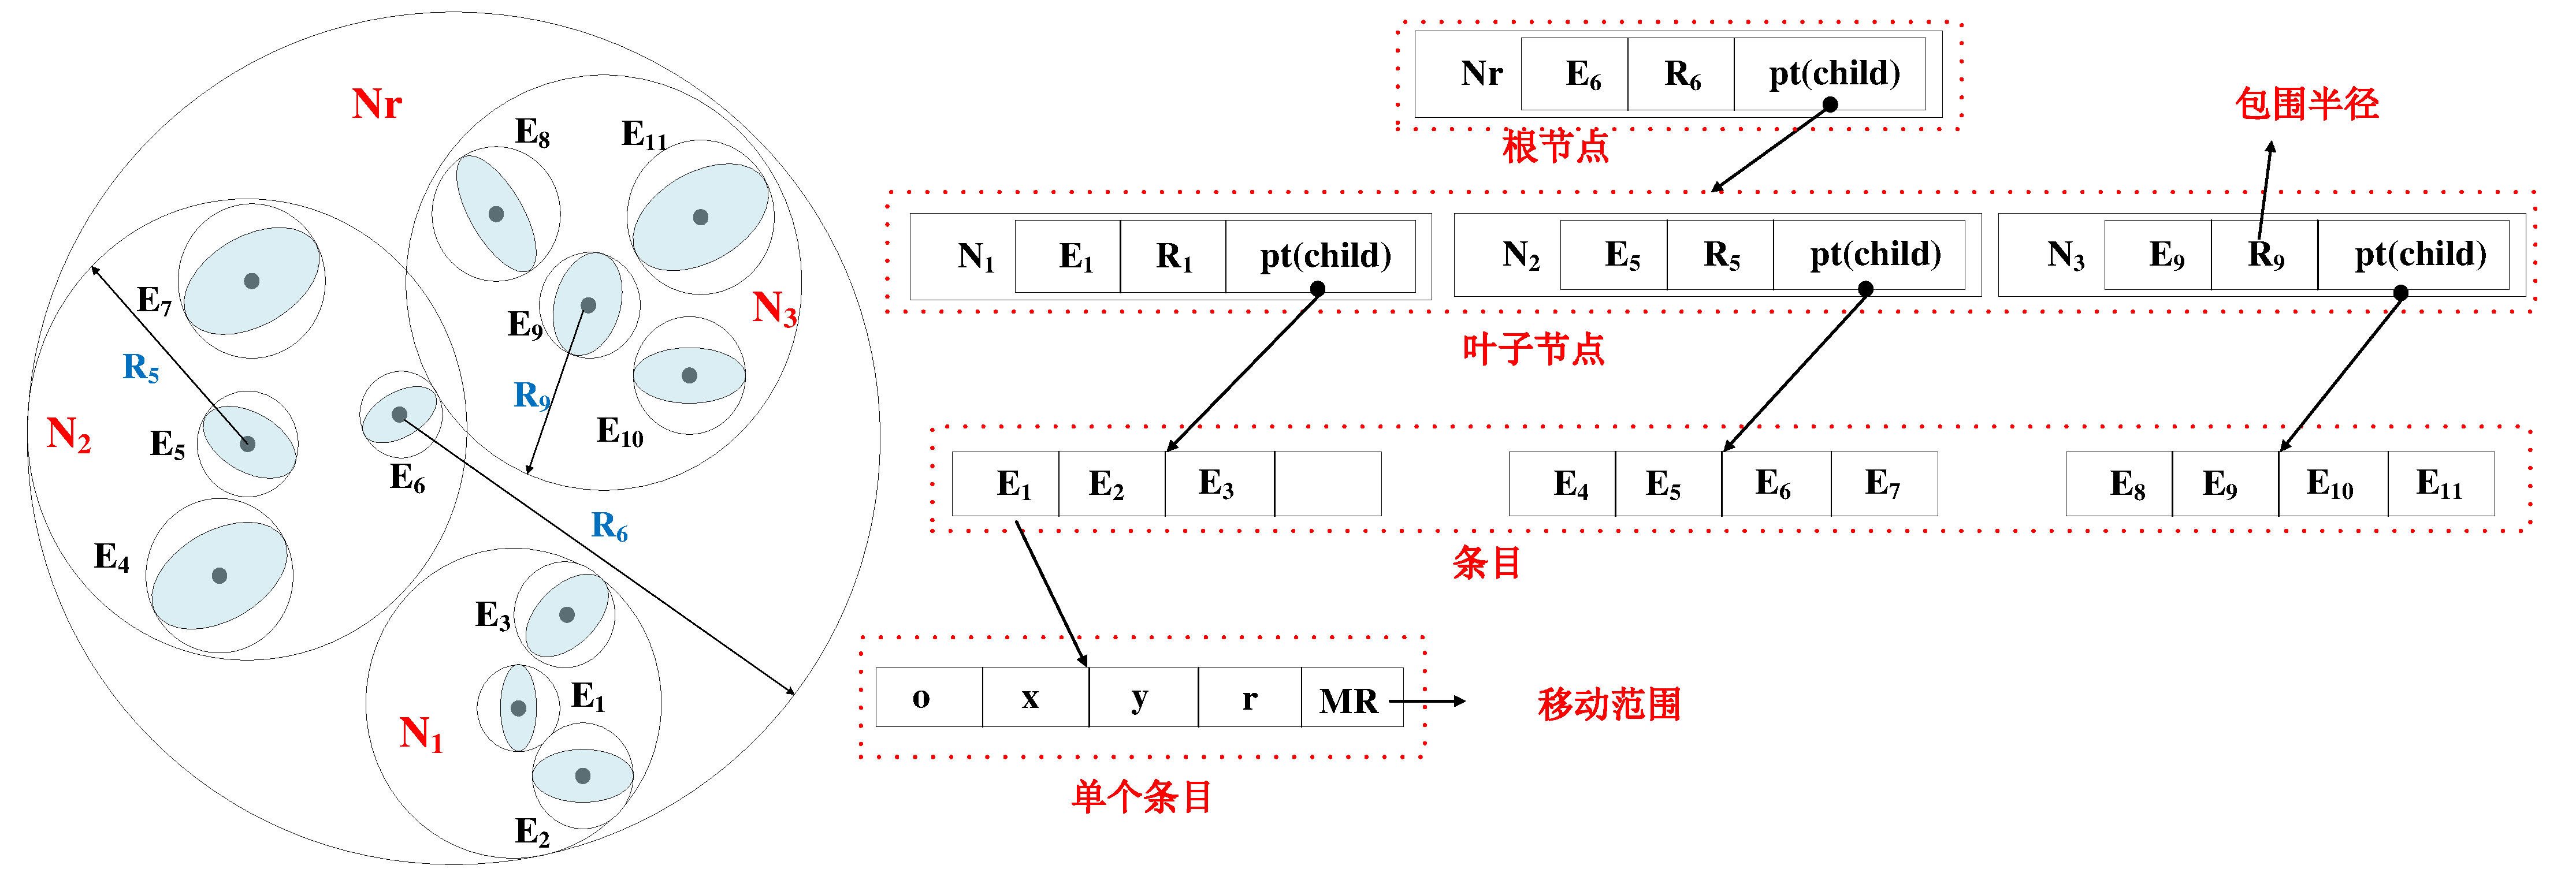
\includegraphics[width=1\textwidth]{fig/section6/mtree.pdf}
\caption{M*-树的结构}
\label{fig:m*-tree}
\end{figure}

\subsection{M*-树}

图~\ref{fig:m*-tree} 展示了 M*-树的结构，其指定容量为 $M=4$，表示每个叶节点的最大条目数。近似圆被视为单独的条目，并独立存储在叶节点中。我们使用近似圆表示时间区间的运动范围，并在 M*-树中对其进行索引。每个圆存储为条目 $E=\{o,x,y,r,MR(o,I)\}$，其中 $o$ 为对象标识，$(x, y)$ 表示圆心，$r$ 为半径，$MR(o,I)$ 包含时间区间的运动范围。M*-树中的每个节点 $N$ 选择叶节点中的一个条目 $E$ 作为其路由对象，格式为 $N=\{E,R,pt(child)\}$。这里，$E$ 是路由对象，$R$ 是能够覆盖 $N$ 中所有条目（即圆）的半径，$pt(child)$ 是指向子节点的指针。需要注意的是，M*-树在条目插入策略、节点分裂策略和路由对象选择策略上遵循了已有研究~\cite{DBLP:conf/edbt/ZhangRSL21,DBLP:conf/vldb/CiacciaPZ97} 的做法，并将这些策略适配到 M*-树结构中。

值得注意的是，同一 M*-树内的时间区间运动范围在时间上是对齐的。我们为特定时间区间索引所有运动范围，当时间区间改变时，需要重建 M*-树索引。

\subsection{交集检查}

我们从查询条目 $E_q=(q, x_q, y_q, r_q, MR(q,I))$ 和 M*-树的根节点开始。目标是检索所有可能与 $E_q$ 相交的条目 $E=\{o, x, y, r, MR(o,I)\}$。为了确定潜在交集，我们计算查询对象 $q$ 与每个条目 $E$ 之间的距离 $d(q, E)=\sqrt{(x_q-x)^2+(y_q-y)^2}$。如果 $d(q, E) \leq r + r_q$，则时间区间运动范围 $MR(q,I)$ 和 $MR(o,I)$ 可能相交。其中，$r$ 和 $r_q$ 分别表示条目 $E$ 和 $E_q$ 的半径。对于每个查询对象 $q$，我们索引所有满足 $d(q,E)\leq r+r_q$ 的条目，并将对应的 $(q,o)$ 加入候选集合，其中 $o$ 是与条目 $E$ 关联的对象标识。

\subsection{算法细节}
\begin{algorithm}[!h]
    \caption{$MBJ(\mathcal{A},\mathcal{B},N_r, I,\epsilon,\theta)$}
    \label{alg:MBJ-Join}
    
    \Input{
    两组移动对象，$\mathcal{A}$ 和 $\mathcal{B}$；\newline
    M*-树的根节点 $N_r$；\newline
    时间间隔 $I$；\newline
    分区参数 $\epsilon$；\newline
    交集相似度阈值 $\theta$。
    }
    \Output{
    $\mathcal{R} = \{(o,o') \mid IS(o,o',I,\epsilon) \geq \theta, (o,o') \in \mathcal{A} \times \mathcal{B}\}$。
    }
    
    \textbf{初始化:} $\mathcal{R} \leftarrow \emptyset$；
    
    \For(\tcc*[f]{遍历集合 $\mathcal{A}$}){$o \in \mathcal{A}$}{
        $\mathcal{L} \leftarrow \{N_r\}$；
    
        \While(\tcc*[f]{M*-树遍历}){$\mathcal{L} \neq \emptyset$}{
            $N \leftarrow \mathcal{L}.pop()$；
    
            \If(\tcc*[f]{非叶子节点}){$N$ 是非叶子节点}{
                \For(\tcc*[f]{遍历子节点}){$N_c \in N.pt(child)$}{
                    \If{$d(o, N_c) \leq N_c.R + o.r$}{
                        $\mathcal{L}.push(N_c)$；
                    }
                }
            }
            \Else(\tcc*[f]{叶子节点处理}){
                \If{$d(o, N) > N.R + o.r$}{
                    $prune(o, N.o)$;\tcp*[f]{预检查策略}
                }
    
                \If{$IS(o, N.o, I, \epsilon) \geq \theta$}{
                    $\mathcal{R} \leftarrow \{\mathcal{R}, (o, N.o)\}$;\tcp*[f]{精炼步骤}
                }
            }
        }
    }
    \textbf{return} $\mathcal{R}$；
    \end{algorithm}
    
    算法~\ref{alg:MBJ-Join} 给出了基于 M*-树的两阶段剪枝匹配算法（MBJ-Alg）的伪代码。算法的输入包括两个移动对象集合、M*-树的根节点、带分区参数 $\epsilon$ 的时间区间，以及相似度阈值 $\theta$。我们使用列表 $\mathcal{R}$ 存储所有满足条件的对象对，初始时 $\mathcal{R}$ 为空（第 1 行）。  

    该算法由两个阶段组成：(1) 基于 M*-树的预检查（第 3--12 行），以及 (2) 精炼过程（第 13--14 行）。在预检查阶段，我们根据 M*-树获取候选对象集合。我们使用列表 $\mathcal{L}$ 存储可能与移动对象相交的节点，初始时 $\mathcal{L}$ 仅包含根节点（第 3 行）。  
    
    当 $\mathcal{L}$ 非空时，我们从中取出与对象 $o$ 的距离 $d(o,N)$ 最小的 M*-树节点 $N$（第 5 行）。如果 $N$ 不是叶节点，则考虑其子节点。对于 $N$ 的每个子节点 $N_c$，我们检查 $o$ 与 $N_c$ 之间的距离。如果该距离不大于 $o$ 与 $N_c$ 半径之和，则将 $N_c$ 压入优先队列（第 7--9 行）。  
    
    如果 $N$ 是叶节点，且 $d(o,N) > N.R + o.r$，则可以安全地剪枝 $(o, N.o)$（第 11--12 行）。当交集相似度不小于阈值 $\theta$ 时，我们通过将 $(o, N.o)$ 添加到结果集来更新 $\mathcal{R}$（第 14 行）。  
    
    最后，返回 $\mathcal{R}$ 作为得到的交集对象对（第 15 行）。

    \subsubsection{时间复杂度分析}

    一般来说，构建 M*-树需要 $O(|\mathcal{B}|\times n)$ 的时间，其中 $\mathcal{B}$ 是被 M*-树索引的对象集合，$n$ 是节点分裂操作的次数。具体来说，当由于对象插入导致节点已满时，需要将其分裂为多个节点，这一操作的时间复杂度为 $O(|\mathcal{B}|)$。值得注意的是，实际构建时间可能会因数据分布等因素而有所不同。  
    
    设 $\mathcal{A}$ 为查询对象集合。为了找到所有候选对象，过滤过程的时间复杂度为 $O(|\mathcal{A}|\times\log|\mathcal{B}|)$。若时间点运动范围内的 POI 平均数量为 $p$，则每次计算 $IS(o,o',I,\epsilon)$ 的时间复杂度为 $O(|I|/\epsilon \times p)$。  
    
    设 $\mathcal{C}$ 为候选对象集合。对候选对象进行精炼的时间复杂度为 $O(|\mathcal{C}|\times |I|/\epsilon \times p)$。  
    
    因此，MBJ-Alg 每轮执行的总时间复杂度为
    \[
    O\big(|\mathcal{B}|\times n + |\mathcal{A}|\times\log|\mathcal{B}| + |\mathcal{C}|\times |I|/\epsilon \times p\big)。
    \]

    \section{Top-$k$ 交集相似度连接}

我们的方法可以很容易扩展以支持 top-$k$ 交集相似度连接（$k$-IS-Join），定义如下。与普通 IS-Join 不同，$k$-IS-Join 不需要阈值参数，而是返回两个集合中前 $k$ 个最相似的轨迹对。

\begin{definition}[$k$-IS-Join]\label{defi:k-IS-Join}
Top-\underline{k} \underline{交}集 \underline{相}似度连接（$k$-IS-Join）从两个对象集合中找到 $k$ 个最相似的对象对集合 $\mathcal{R}$，即 $|\mathcal{R}|=k$，且满足 $\forall (o_i,o_j)\in \mathcal{R} (\forall (o_i^{'},o_j^{'})\in (\mathcal{A}\times \mathcal{B})\setminus \mathcal{R}$，有
$(IS(o_i,o_j,I,\epsilon)>IS(o_i^{'},o_j^{'},I,\epsilon)))$。
\end{definition}

算法~\ref{alg:kMBJ-Join} 和算法~\ref{alg:kHBJ-Join} 分别给出了基于 M*-树和 HBall-树的 $k$-IS-Join 解法。


\begin{algorithm}[!h]
    \caption{$kMBJ(\mathcal{A},\mathcal{B},N_r,I,\epsilon,k)$}
    \label{alg:kMBJ-Join}
    
    \Input{
    两个移动对象集合，$\mathcal{A}$ 和 $\mathcal{B}$；\newline
    M*-树的根节点 $N_r$；\newline
    时间区间 $I$；\newline
    分区参数 $\epsilon$；\newline
    参数 $k$。
    }
    \Output{
    $\mathcal{R} =$ top-$k$ 对象对。
    }
    
    \textbf{初始化:} $\mathcal{R} \leftarrow$ 大小为 $k$ 的优先队列 PriorityQueue$\langle (o,o'), sim \rangle$；
    
    \For(\tcc*[f]{遍历集合 $\mathcal{A}$}){$o \in \mathcal{A}$}{
        $\mathcal{L} = N_r.query(MR(o,I))$；
    
        \For(\tcc*[f]{遍历候选对象}){$o' \in \mathcal{L}$}{
            $sim_k = \mathcal{R}.top().sim$；
    
            \If{$|\mathcal{R}| < k$}{
                $\mathcal{R}.push((o,o'), sim)$；
            }
            \ElseIf{$IS(o,o',I,\epsilon) \geq sim_k$}{
                $\mathcal{R}.push((o,o'), sim)$；
                $\mathcal{R}.poll()$；
            }
        }
    }
    
    \textbf{return} $\mathcal{R}$；
    \end{algorithm}



\begin{algorithm}[!h]
    \caption{$kHBJ(\mathcal{A},\mathcal{B},N_r,I,\epsilon,k)$}
    \label{alg:kHBJ-Join}
    
    \Input{
    两个移动对象集合，$\mathcal{A}$ 和 $\mathcal{B}$；\newline
    HBall-树的根节点 $N_r$；\newline
    时间区间 $I$；\newline
    分区参数 $\epsilon$；\newline
    参数 $k$。
    }
    \Output{
    $\mathcal{R} =$ top-$k$ 对象对。
    }
    
    \textbf{初始化:} $\mathcal{R} \leftarrow$ 大小为 $k$ 的优先队列 PriorityQueue$\langle (o,o'), sim \rangle$；
    
    \For(\tcc*[f]{遍历集合 $\mathcal{A}$}){$o \in \mathcal{A}$}{
        $\mathcal{L} = N_r.query(MR(o,I))$；
    
        \For(\tcc*[f]{遍历候选对象}){$o' \in \mathcal{L}$}{
            $sim_k = \mathcal{R}.top().sim$；
    
            \If{$|\mathcal{R}| < k$}{
                $\mathcal{R}.push((o,o'), sim)$；
            }
            \Else{
                \If{$IS(o,o',I,\epsilon)_{ub}^{'} < \theta$}{
                    \textbf{continue}；\tcp*[f]{时间点剪枝}
                }
                \If{$IS(o,o',I,\epsilon) \geq sim_k$}{
                    $\mathcal{R}.push((o,o'), sim)$；
                    $\mathcal{R}.poll()$；
                }
            }
        }
    }
    
    \textbf{return} $\mathcal{R}$；
    \end{algorithm}



\section{IS-Join 的附加实验}

\subsubsection{相似度阈值的影响}
对于 HBJ-Alg，增加相似度阈值 $\theta$ 可以提高剪枝效果。较大的 $\theta$ 减少搜索空间，从而降低 CPU 时间和访问的时间区间运动范围数量。图~\ref{img:vary_sim_ftime} 展示了在改变相似度阈值时的效率表现。与 MBJ-Alg 对比，HBJ-Alg 在所有设置下均优于 MBJ-Alg，运行时间最多可提升 3 倍。虽然 HBJ-Alg 在较高阈值下运行时间略有下降，但 MBJ-Alg 和 HBJ-Alg\# 的趋势不明显。

\begin{figure}[tb]
    \centering
    \subfloat[]{
        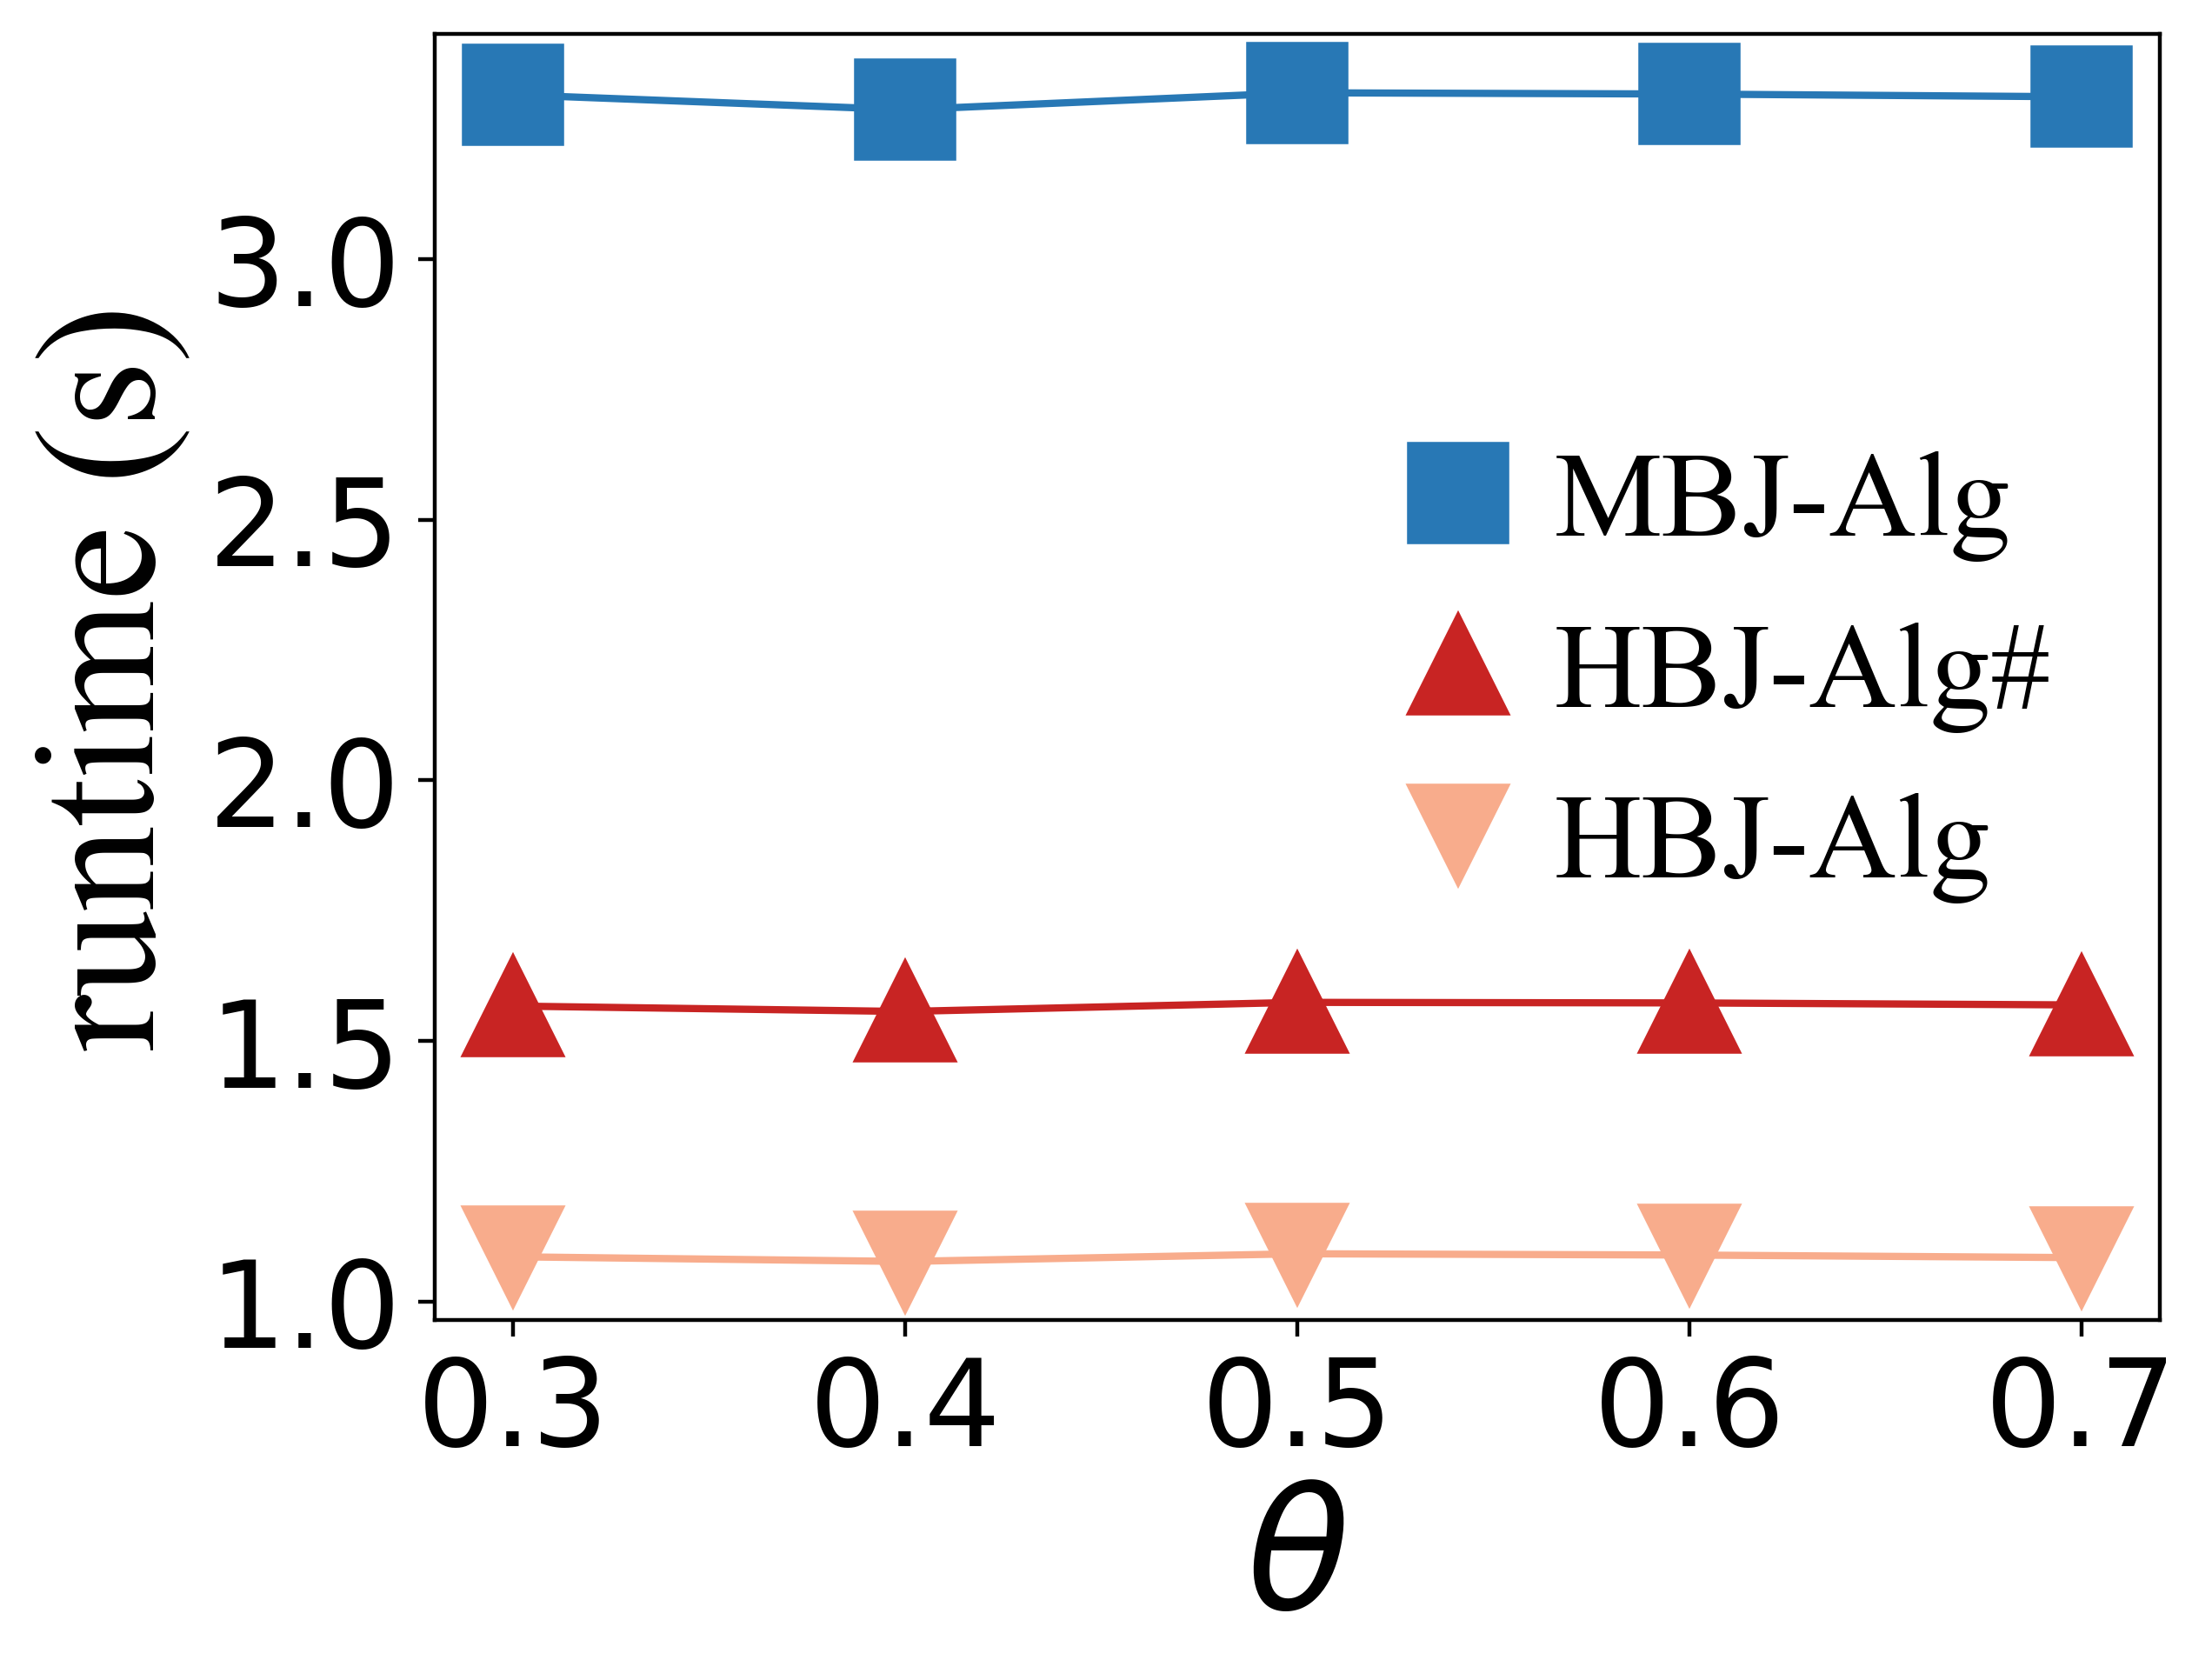
\includegraphics[width=0.4\textwidth]{fig/section6/geo-sim-ftime.png}
        \label{geo-sim-totaltime}
    }%
    \hfill
    \subfloat[]{
        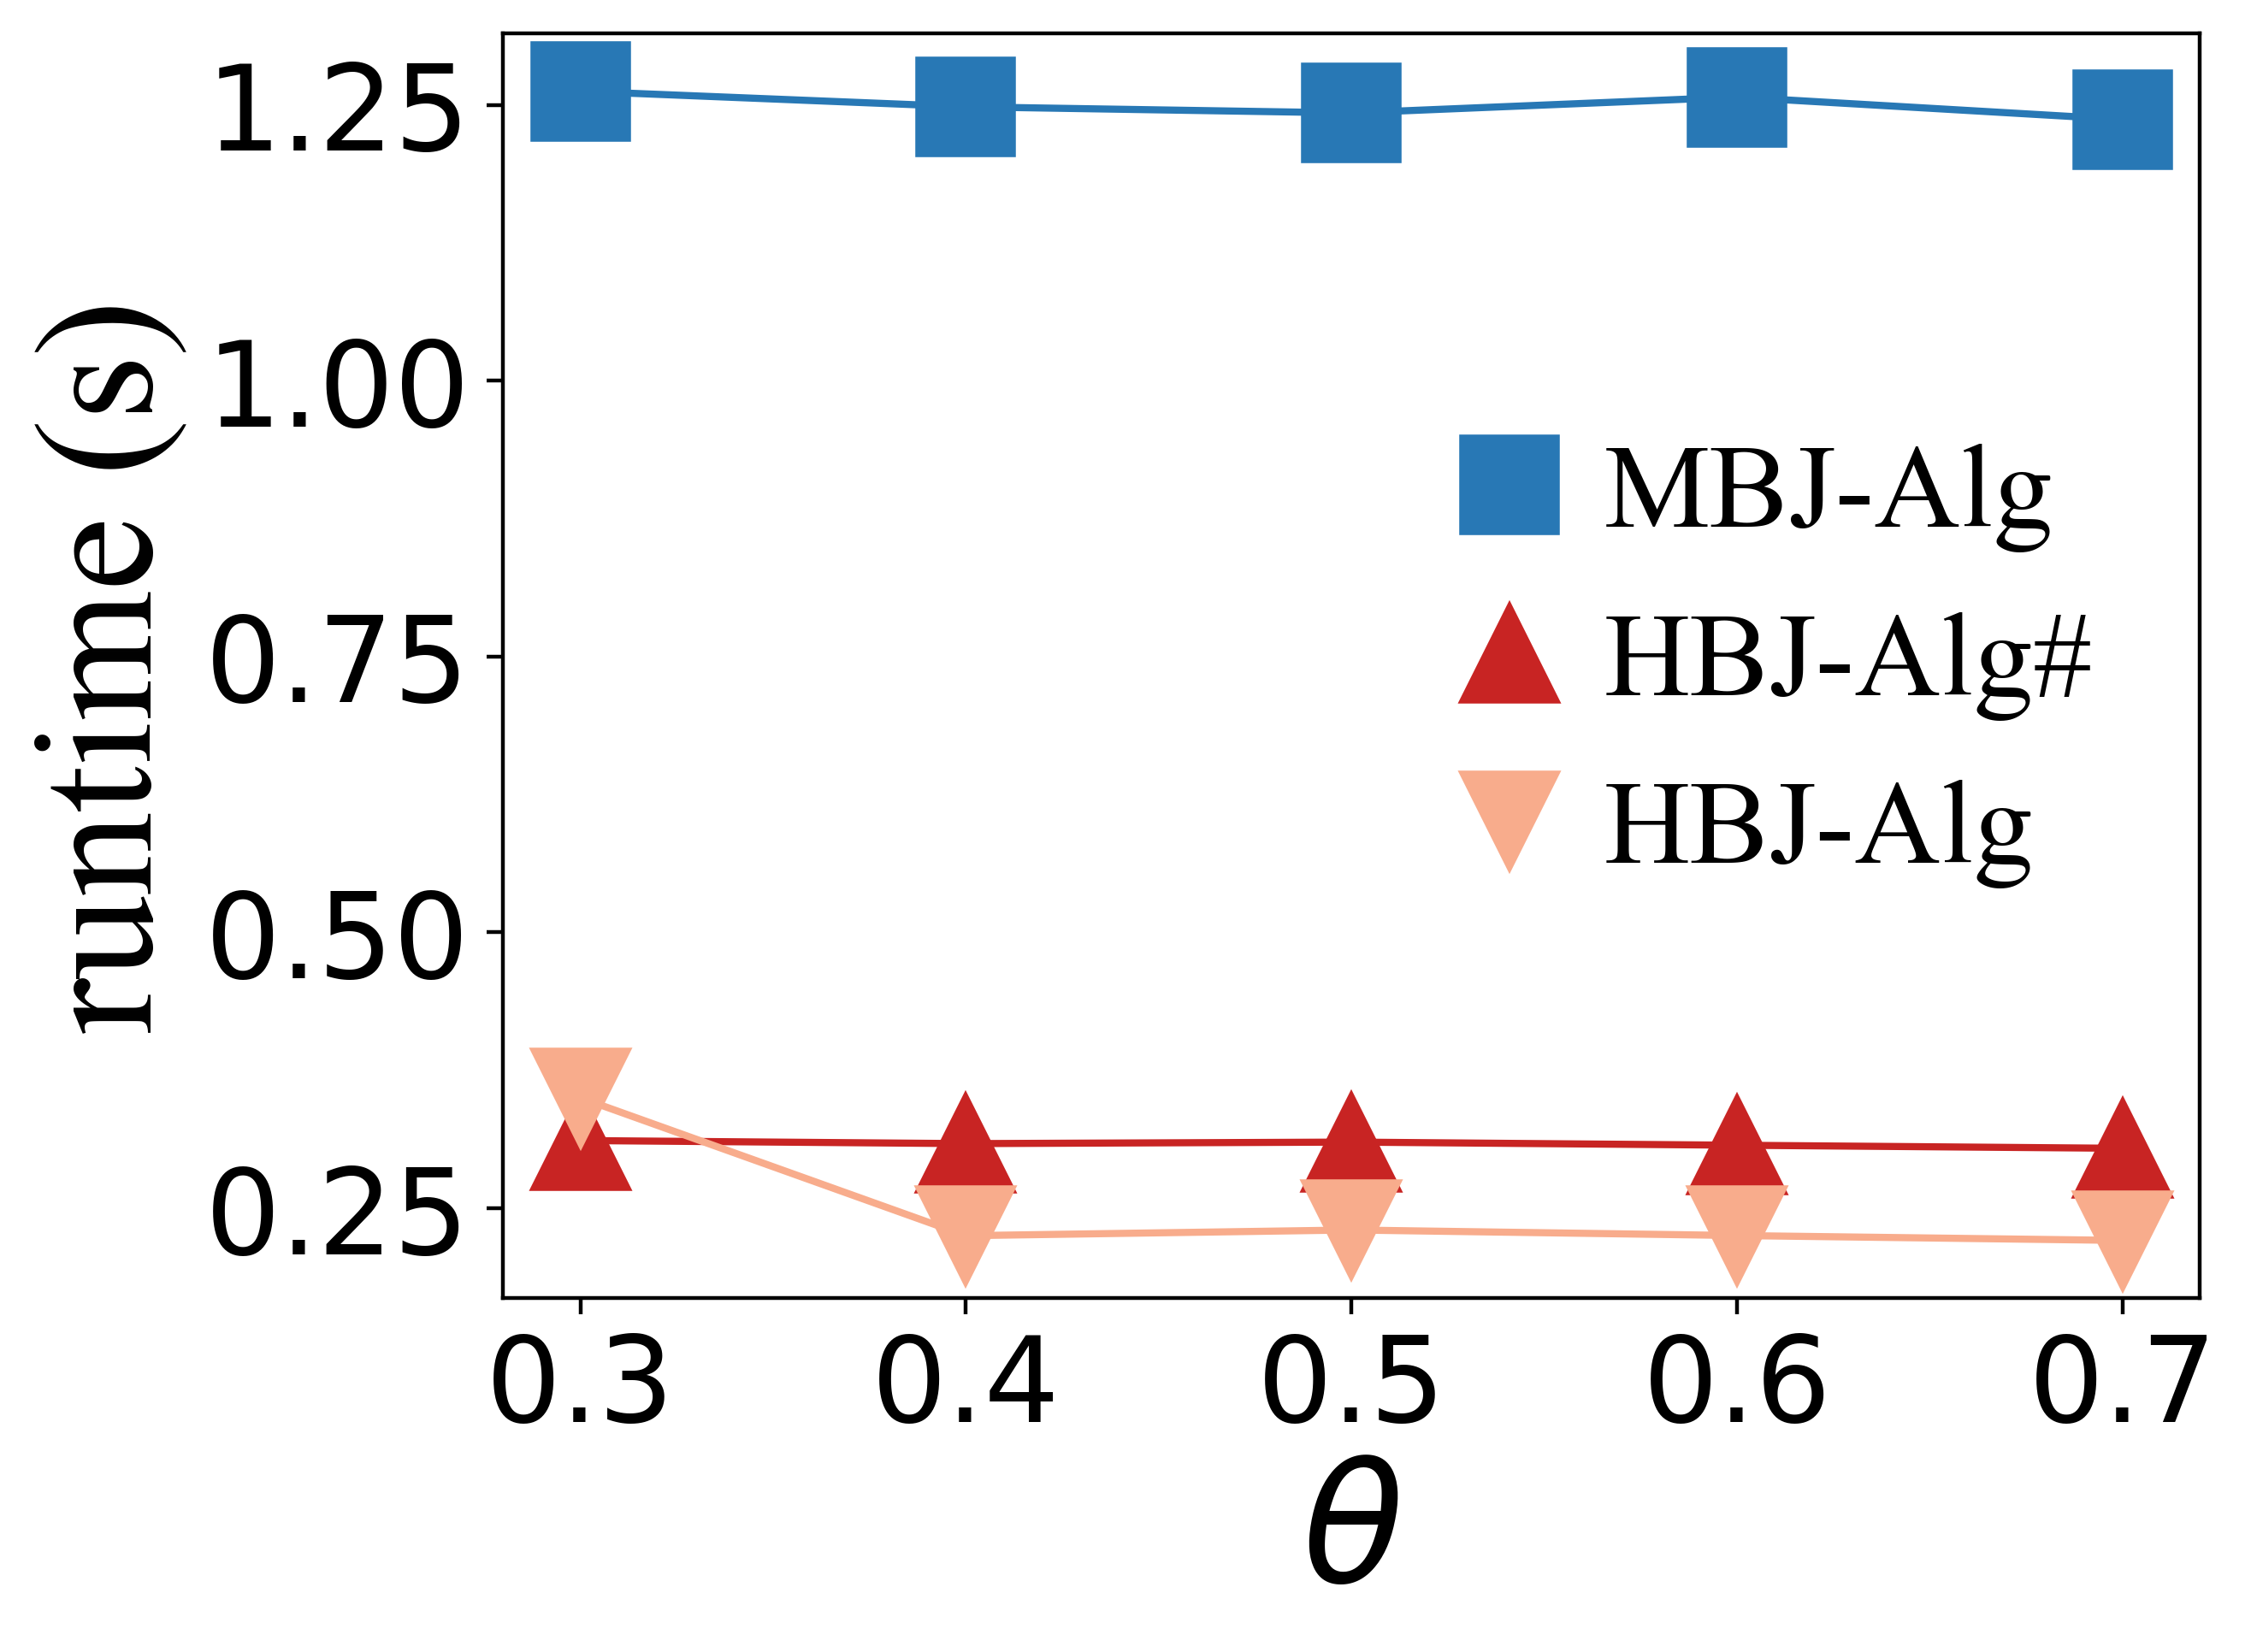
\includegraphics[width=0.4\textwidth]{fig/section6/pt-sim-ftime.png}
        \label{pt-sim-totaltime}
    }%
    \caption{相似度阈值的影响 \subref{geo-sim-totaltime}:Geolife数据集下的实验; \subref{pt-sim-totaltime}:Porto数据集下的实验}
    \label{img:vary_sim_ftime}
\end{figure}

\subsubsection{重新分区策略的评估}
我们比较 HBJ-Alg 和 HBJ-Alg$*$ 的性能，主要指标为节点访问总次数。图~\ref{img:vary_num_access} 显示了移动对象数量对重新分区策略性能的影响（默认设置）。随着移动对象数量增加，节点访问总数也增加。HBJ-Alg 与 HBJ-Alg$*$ 的性能差距随对象数量增长而扩大。HBJ-Alg 的重新分区策略可在不增加索引构建时间的情况下，将节点访问数减少约 10\%，甚至可能降低索引构建时间（见图~\ref{img:vary_num_ctime}）。因此，重新分区策略有助于提升整体效率，处理大规模数据集时更有效。

\begin{figure}[tb]
    \centering
    \subfloat[]{
        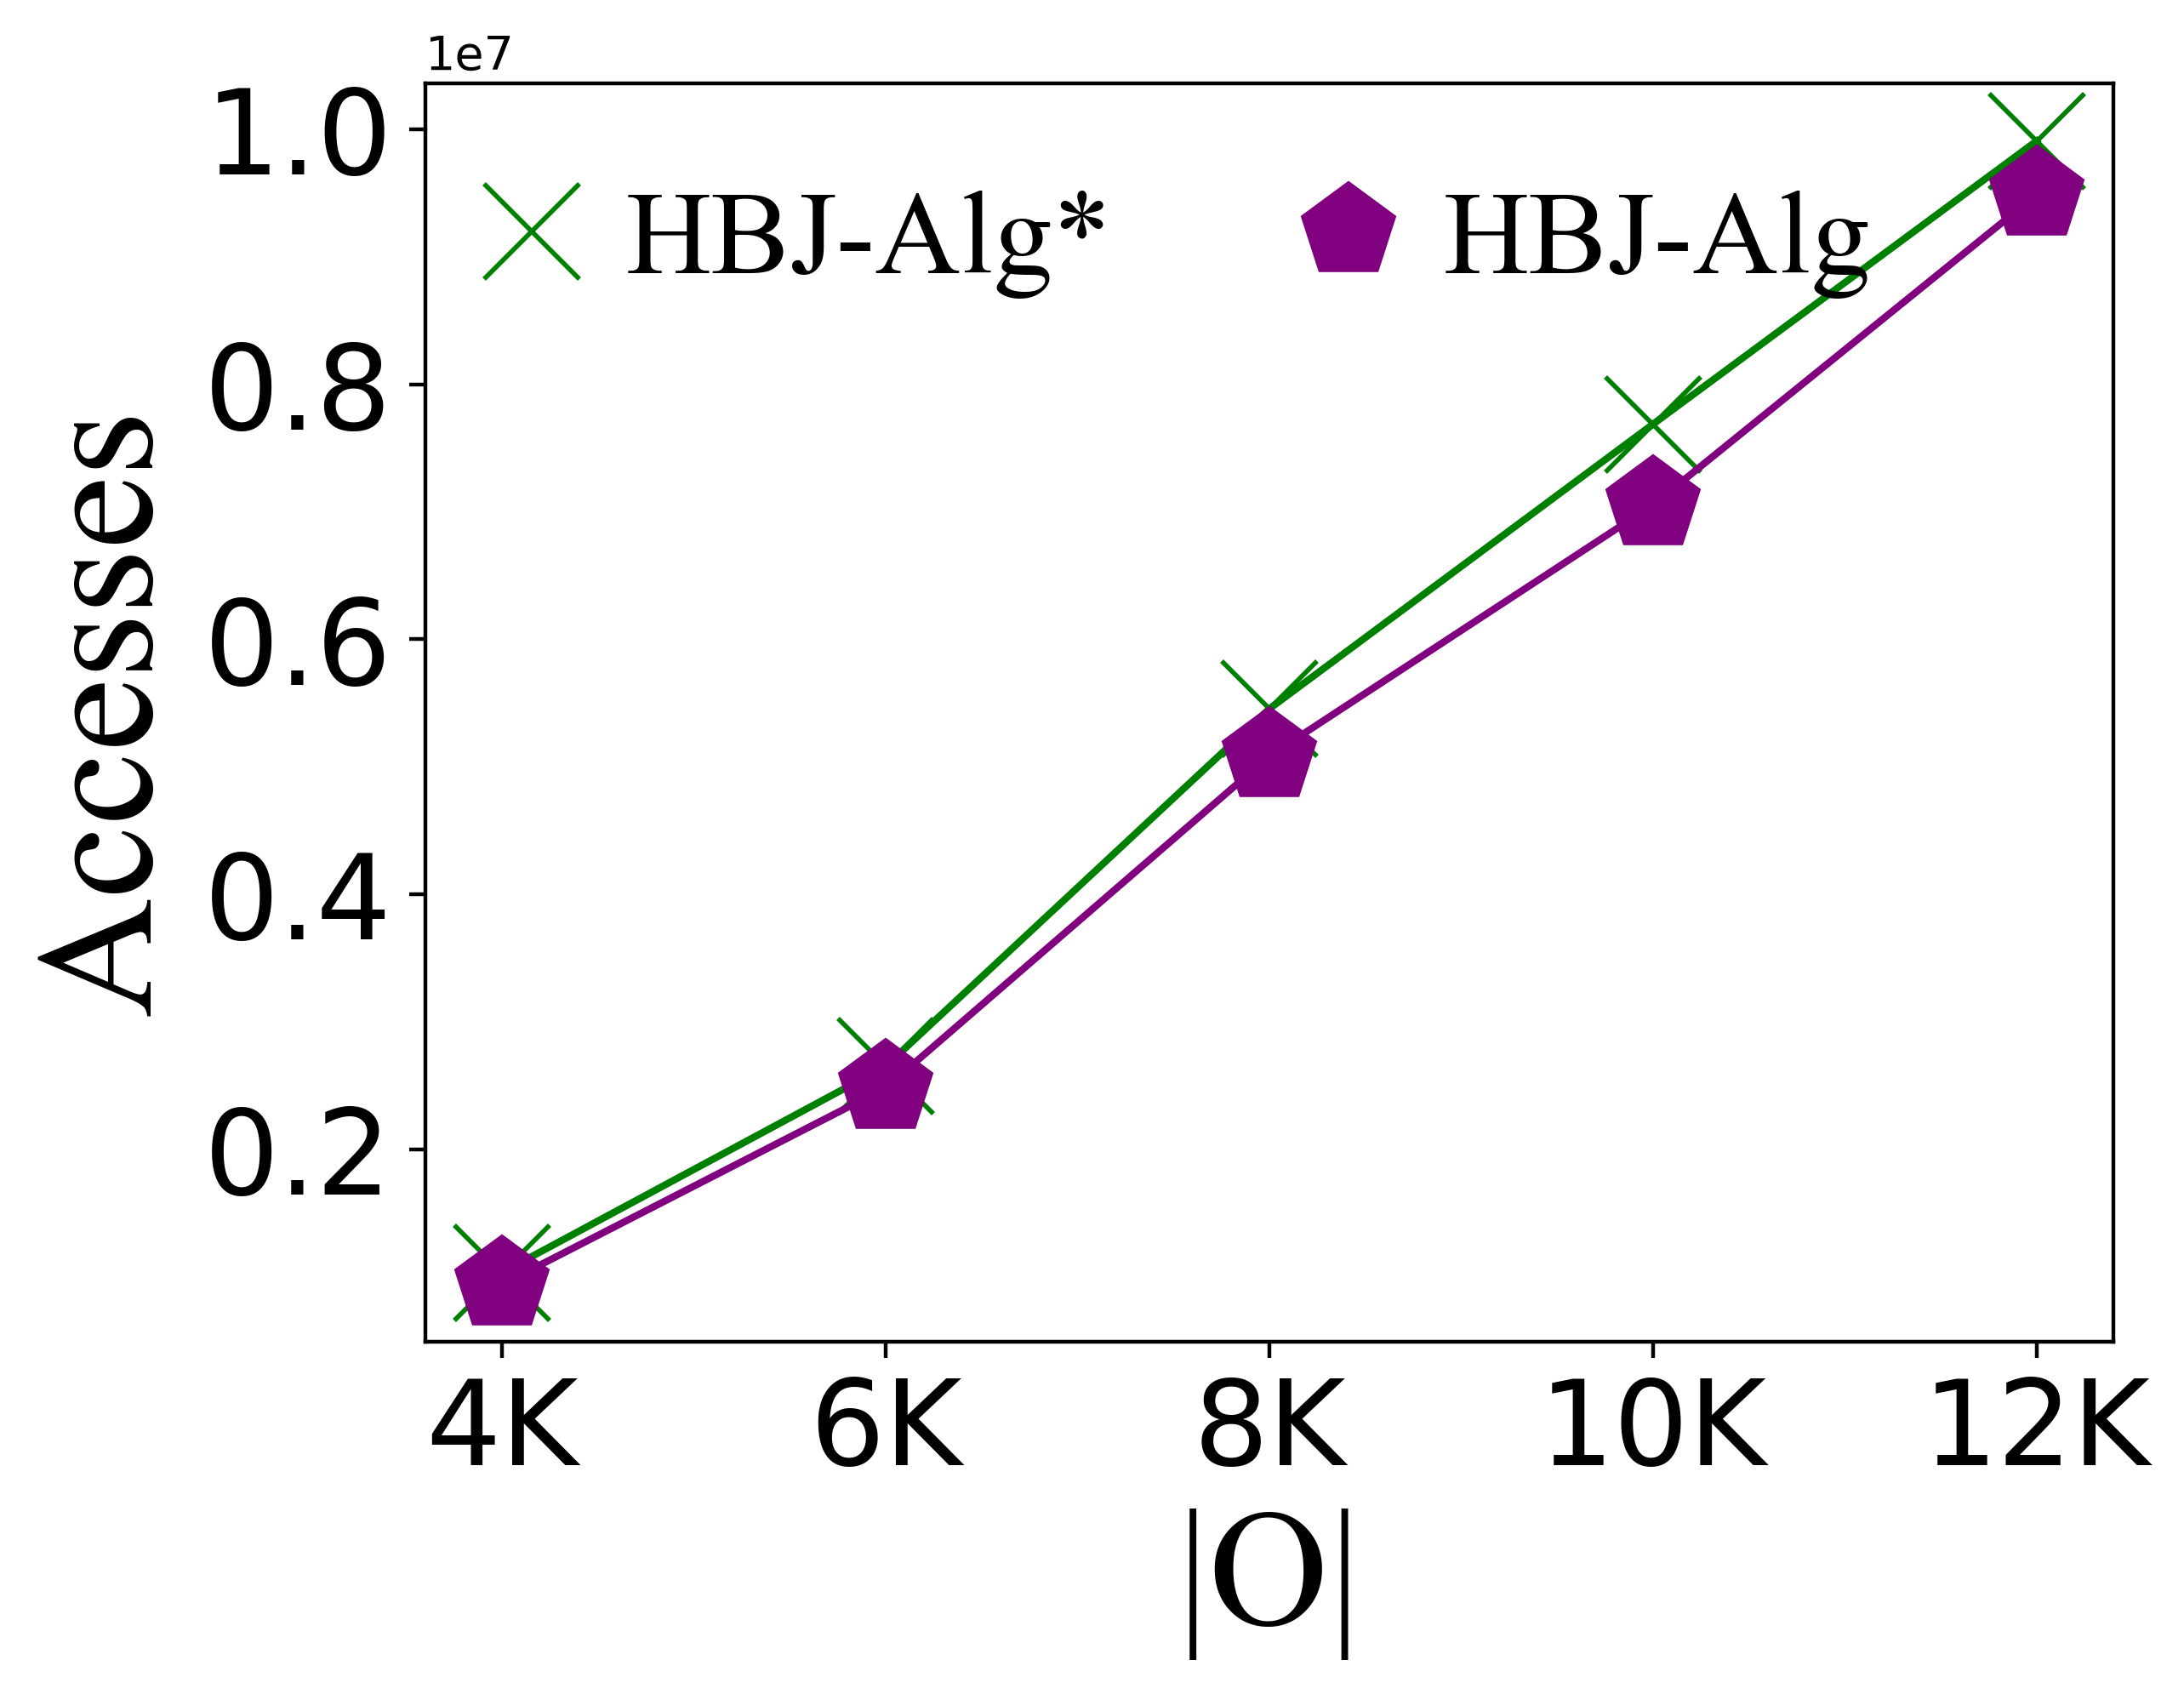
\includegraphics[width=0.4\textwidth]{fig/section6/geo-num-access.png}
        \label{geo-num-access}
    }%
    \hfill
    \subfloat[]{
        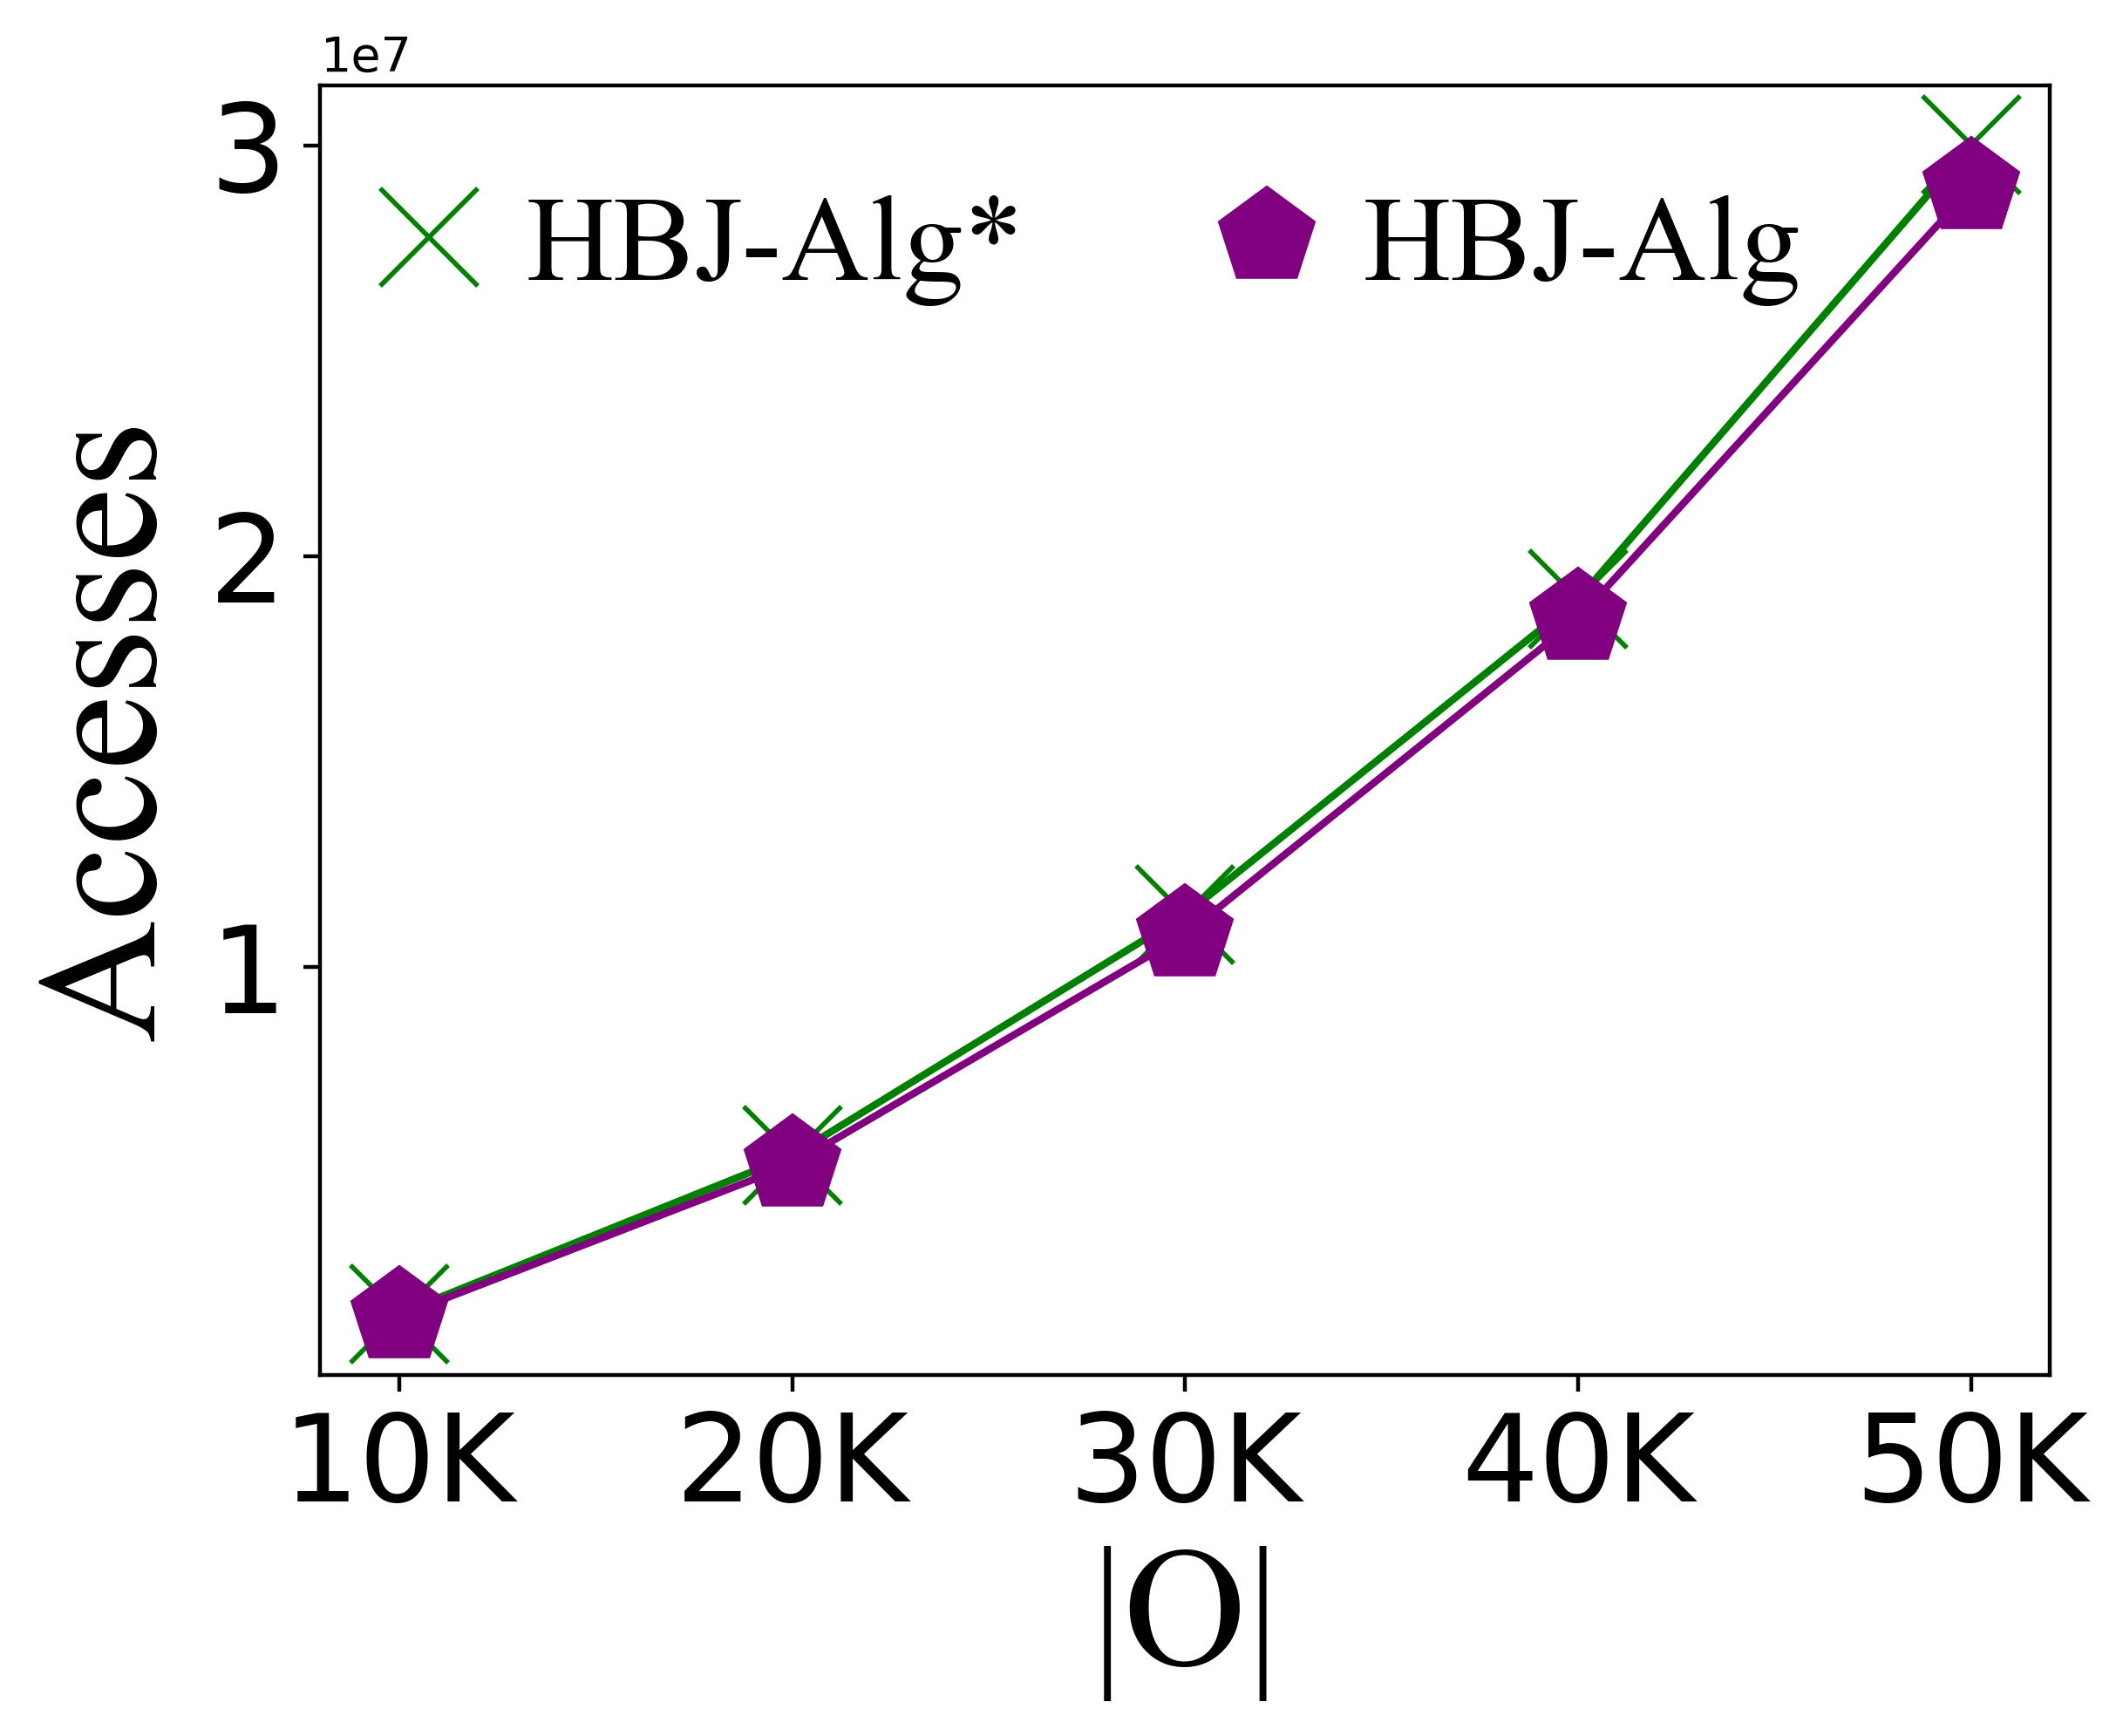
\includegraphics[width=0.4\textwidth]{fig/section6/pt-num-access.png}
        \label{pt-num-access}
    }%
    \caption{移动对象数量对节点访问次数的影响 \subref{geo-num-access}:Geolife数据集下的实验; \subref{pt-num-access}:Porto数据集下的实验}
    \label{img:vary_num_access}
\end{figure}

\subsection{Top-$k$ IS-Join 的实验研究}

\subsubsection{$k$ 的影响}
我们评估算法在 top-$k$ 交集相似度连接中的性能。图~\ref{img:vary_k_ftime} 展示了不同 $k$ 下的效率表现。可以看出，HBJ-Alg 在 Geolife 和 Porto 数据集上的 CPU 时间分别比 MBJ-Alg 提升约 3 倍和 5 倍。这表明我们的方法在 top-$k$ 连接中具有明显优势。

\begin{figure}[tb]
    \centering
    \subfloat[]{
        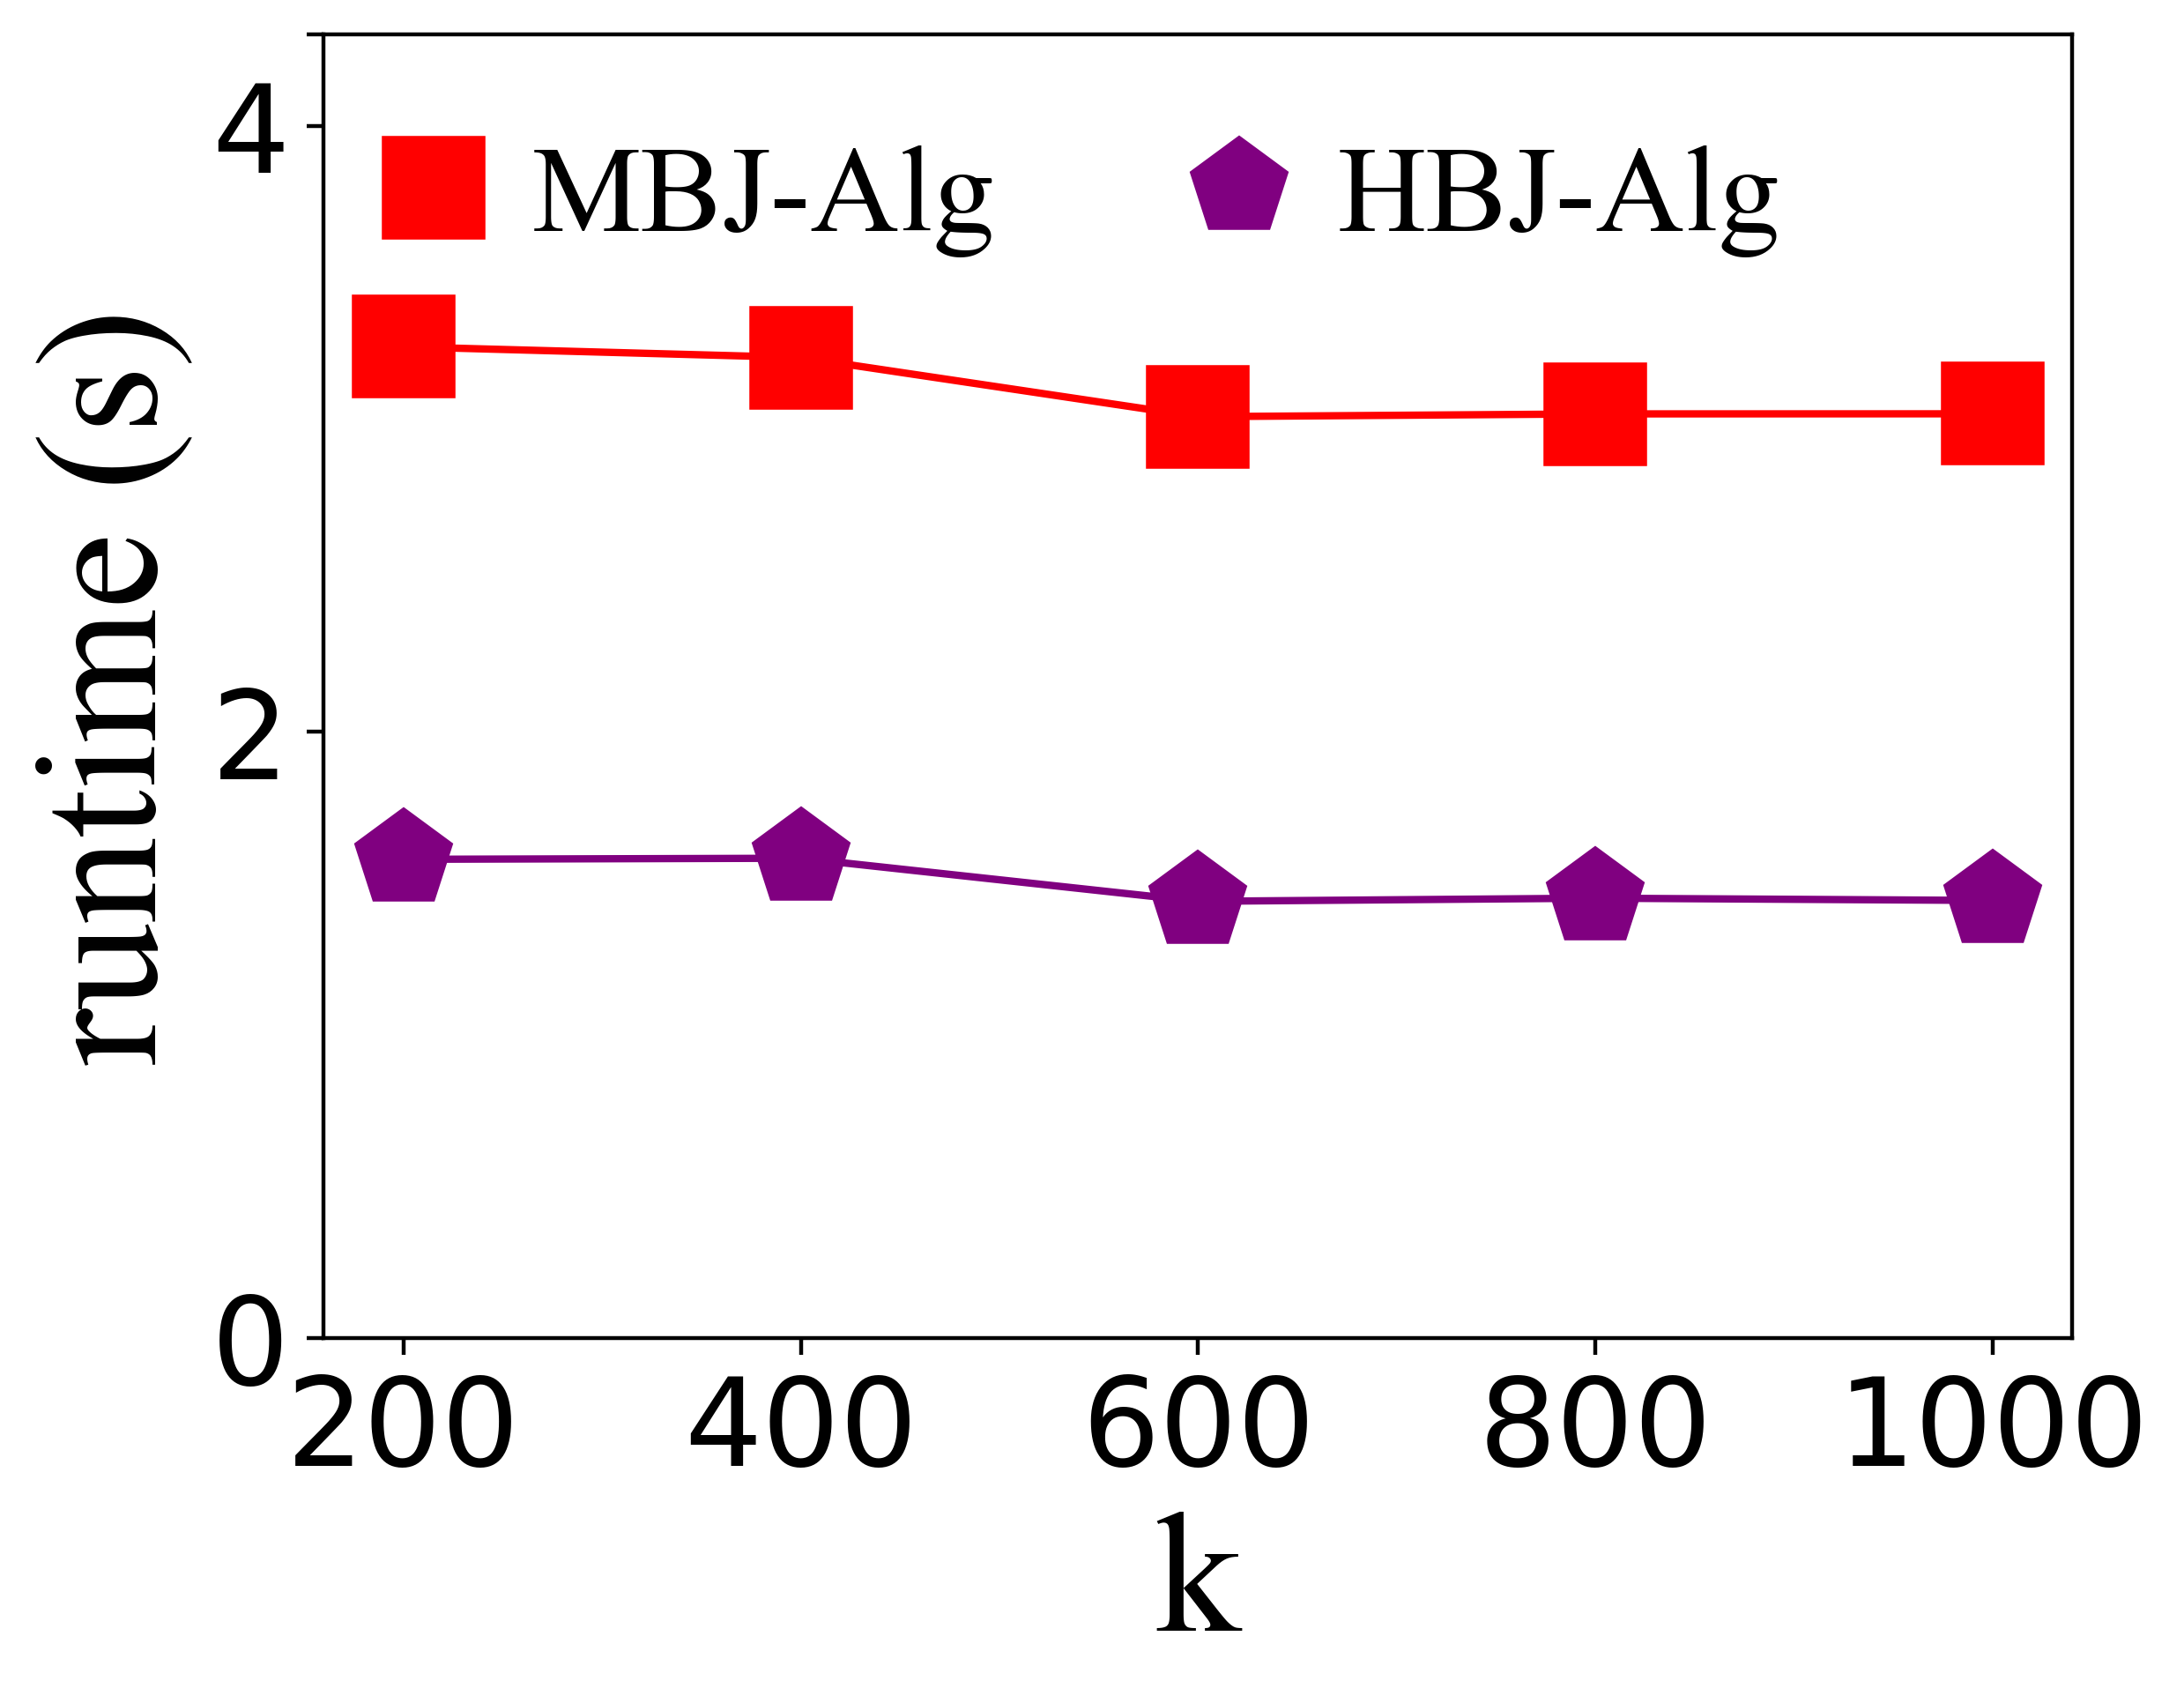
\includegraphics[width=0.4\textwidth]{fig/section6/geo-k-ftime.png}
        \label{geo-k-ftime}
    }%
    \hfill
    \subfloat[]{
        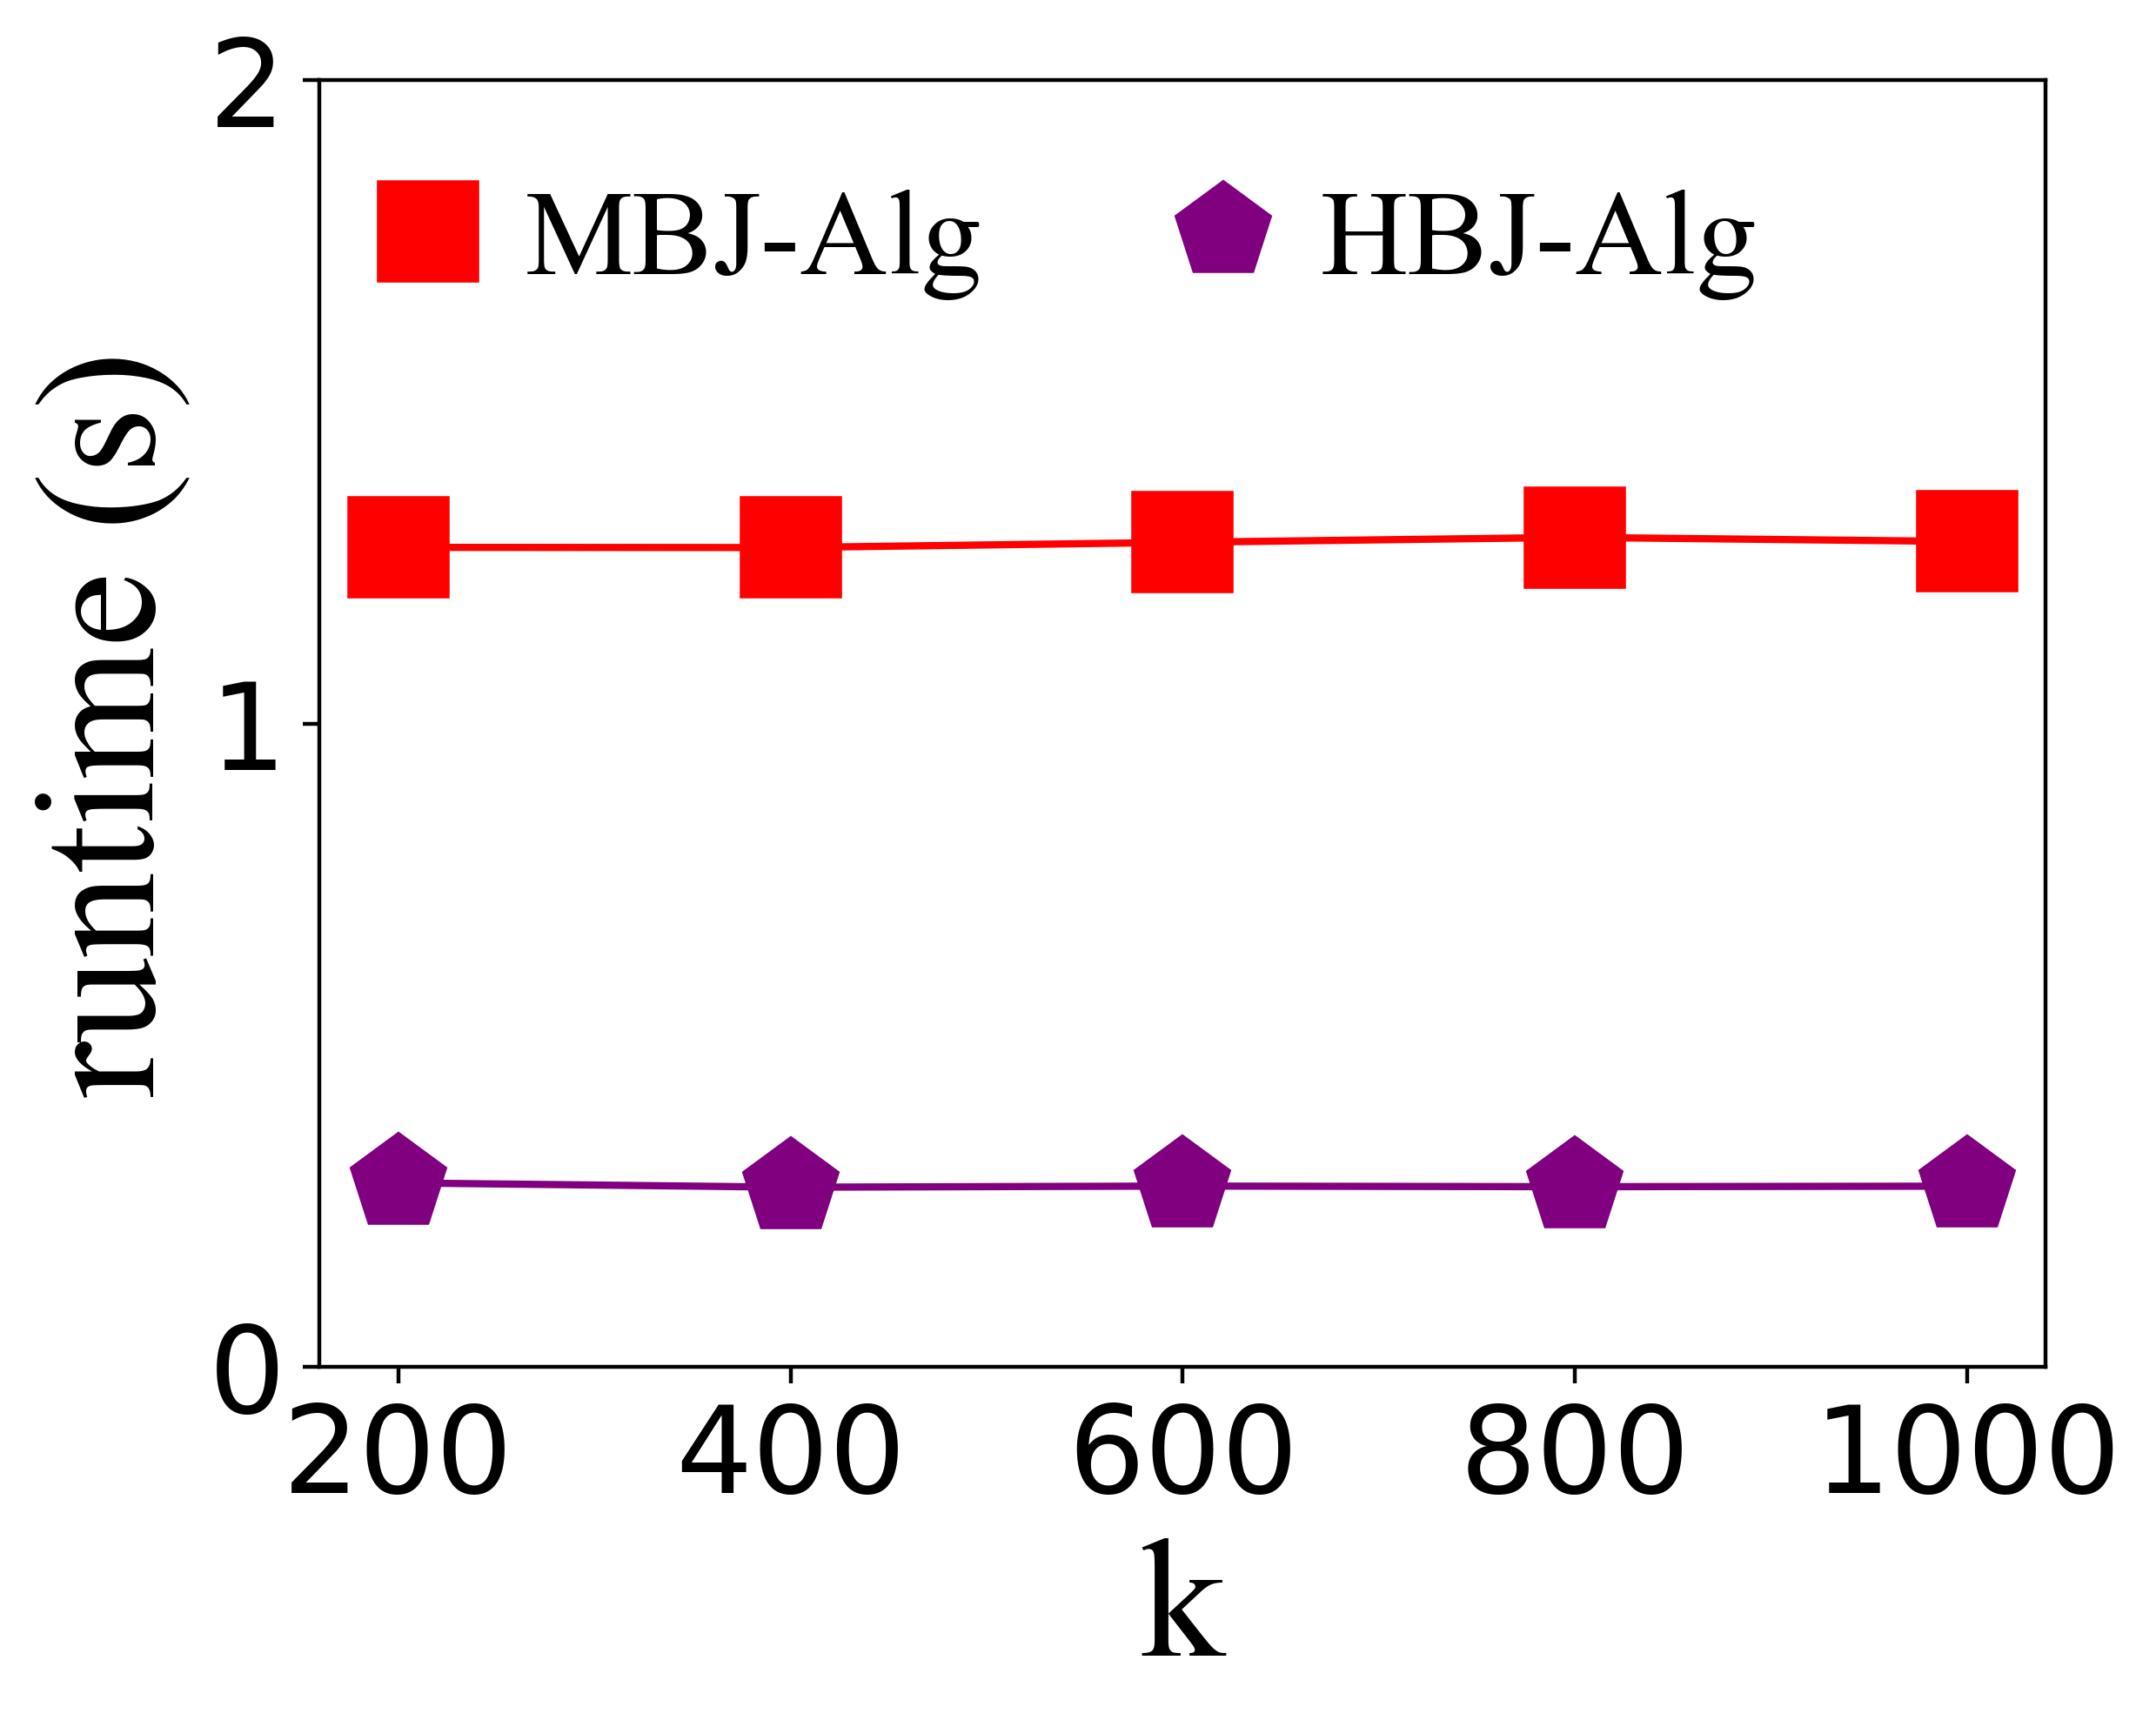
\includegraphics[width=0.4\textwidth]{fig/section6/pt-k-ftime.png}
        \label{pt-k-ftime}
    }%
    \caption{$k$ 的影响 \subref{geo-k-ftime}:Geolife数据集下的实验; \subref{pt-k-ftime}:Porto数据集下的实验}
    \label{img:vary_k_ftime}
\end{figure}

\section{特征精炼}

本节中，我们将时间点运动范围的特征视为面积。第~\ref{sec:refinement} 节介绍了对应的候选对象精炼方法，用于近似交集相似度计算。

\subsubsection{候选对象精炼}
\label{sec:refinement}

精确计算两个时间点运动范围的交集面积非常困难，计算代价高昂 \cite{DBLP:journals/comvis/HughesC12}。为了近似计算时间点交集相似度，我们在时间点运动范围内进行均匀采样。具体方法为，将运动范围包裹在矩形内，在矩形内均匀采样，再用椭圆方程过滤掉矩形外的点。一个更简洁的方法是极坐标采样 \cite{stark1979sampling}。  

具体做法如下：在 $MR(o,t_1)$ 上采样点，并计算落在 $MR(o',t_1)$ 内的点数量 $n_1$；在 $MR(o',t_1)$ 上采样点，并计算落在 $MR(o,t_1)$ 内的点数量 $n_2$。基于此，时间点交集相似度近似计算公式如下（记为 $IS'(o,o',t)$）：

\begin{equation}
    \label{eq:app point sim}
    IS'(o,o',t) = \frac{n_1}{|\mathcal{S}_o|} \times \frac{n_2}{|\mathcal{S}_{o'}|}
\end{equation}

其中，$|\mathcal{S}_o|$ 和 $|\mathcal{S}_{o'}|$ 分别表示对象 $o$ 和 $o'$ 的时间点运动范围的采样点数量。采样点数量与时间点运动范围面积成正比。采样点越多，近似结果越接近真实值，但计算开销也越大。

\begin{figure}[tb]
    \centering
    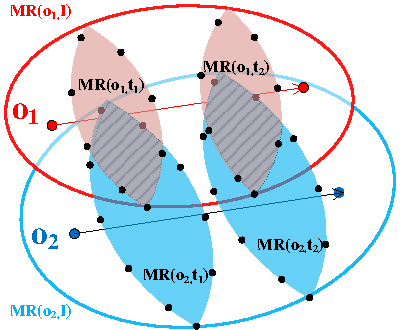
\includegraphics[width=0.6\textwidth]{fig/section6/sample.pdf}
    \caption{时间点运动范围内的采样示意}
    \label{fig:sample}
\end{figure}

\noindent
\textbf{示例. }
图~\ref{fig:sample} 展示了候选对象精炼的示例。假设候选集合 $\mathcal{L}=\{(o_1,o_2)\}$，其时间区间运动范围有交集。将当前时间区间划分为两个时间片 $t_1^\epsilon$ 和 $t_2^\epsilon$。在 $o_1$ 的时间点运动范围上采样 8 个点，在 $o_2$ 上采样 10 个点。  

在 $t_1$ 时，$n_1=3$，$n_2=2$，则根据公式~\ref{eq:app point sim}，$IS'(o,o',t_1)=\frac{3}{8}\times\frac{2}{10}=\frac{3}{40}$。在 $t_2$ 时，$IS'(o,o',t_2)=\frac{4}{8}\times\frac{2}{10}=\frac{1}{10}$。因此，$IS'(o,o',I,\epsilon)=(\frac{3}{40}+\frac{1}{10})/2=\frac{7}{80}$。

\section{本章小结}
本文提出了一种新的面向移动对象的运动范围感知相似连接框架 IS-Join。该框架通过引入对象的潜在运动区域，而非仅依赖离散的轨迹点，有效刻画了对象之间的时空交互关系。不同于传统的轨迹相似连接方法，IS-Join 以运动范围之间的交集相似度为建模对象，使其能够支持更加灵活的查询，适用于交通监控、野生动物追踪以及接触追踪等应用场景。为高效地在大规模数据上处理 IS-Join 查询，我们提出了一种融合重划分策略的 HBall-tree 索引结构，并设计了预检查与剪枝技术，以减少不必要的候选对象对评估，从而显著提升处理效率。基于两个真实世界数据集的大量实验结果表明，与精心设计的基线方法相比，我们的方法在性能上最高可获得约3倍的加速效果。